\section{How to use \toolname as a Coverage Analysis
Tool}\label{sec:coverage}

By default, the tool displays the bytecode instead of the Java
source code, since the source code may not be available. The user
can use the \pk{Visualization} menu to change the display to show
the bytecode or source code, as well as the \DUG of each method in
the current class.  As can be observed in
Figure~\ref{fig:dispenser-bytecode}, \toolname uses different
colors to provide hints to the tester to ease the test generation.
The different colors represent requirements with different
weights, and the weights are calculated based on dominator and
super-block analysis~\cite{Agrawal94DSBP}. Informally, the weight
of a testing requirement corresponds to the number of testing
requirements that will be covered if this particular requirement
is covered. Therefore, covering the requirement with the highest
weight will increase the coverage faster\footnote{Observe that the
weight is calculated
        considering only the coverage information
        and should be seen as hints. It does not
        take into account, for instance, the complexity or
        the criticality of a given part of the program. The tester, based on
        his/her experience may desire to cover first a requirement with a
        lower weight but that has a higher complexity or criticality and then,
        after recomputing the weights, uses the hints provided by \toolname to
        increase the coverage faster.}.
The weight schema is used in all views of a given class/method:
bytecode, source code and \DUG.
Figure~\ref{fig:dispenser-bytecode} shows part of the colored
bytecode of the \pk{Dispenser.dispense()} method before the
execution of any test case and Figure~\ref{fig:dispenser-dug} part
of the \DUG of the same method. The different colors correspond to
the weight of each node, considering the \pk{All-Pri-Nodes}
criterion. Observe that the color bar (below the main menu) goes
from white (weight 0) to red (weight 13).

In our example, observe that the node 105 in
Figure~\ref{fig:dispenser-dug}, composed by bytecote instructions
from 105 to 112 (Figure~\ref{fig:dispenser-bytecode}), is one of
the highest weight. In this way, a test case that exercises node
105 increases the coverage in at least 13. A requirement with
weight zero is a covered requirement and it is painted in white.

Although the source code is not required by \toolname, when it is
available, the corresponding source code of the current class can
also be displayed in colors, mapped back from the bytecode,
facilitating the identification of which part of the code should
be covered first. For example, Figure~\ref{fig:dispenser-source}
shows that the statement on line 24 has the highest priority \wrt
the \pk{All-Pri-Nodes} criterion. By covering this particular
node, at least 13 other nodes will be covered.

\begin{figure}[!ht]
\begin{center}
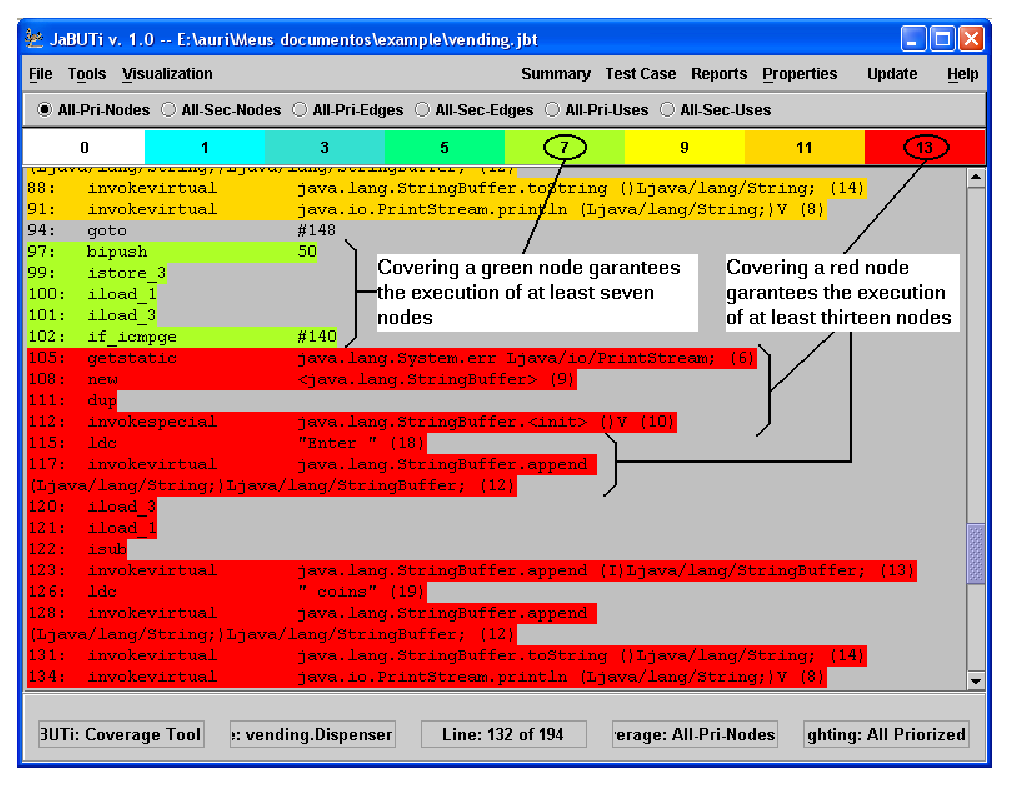
\includegraphics[height=0.40\textheight]{fig/dispenser-bytecode-edited.eps}
\caption{\label{fig:dispenser-bytecode} \pk{Dispenser.dispenser}
method: bytecode prioritized \wrt \pk{All-Pri-Nodes} criterion.}
\end{center}
\end{figure}


\begin{figure}[!ht]
\begin{center}
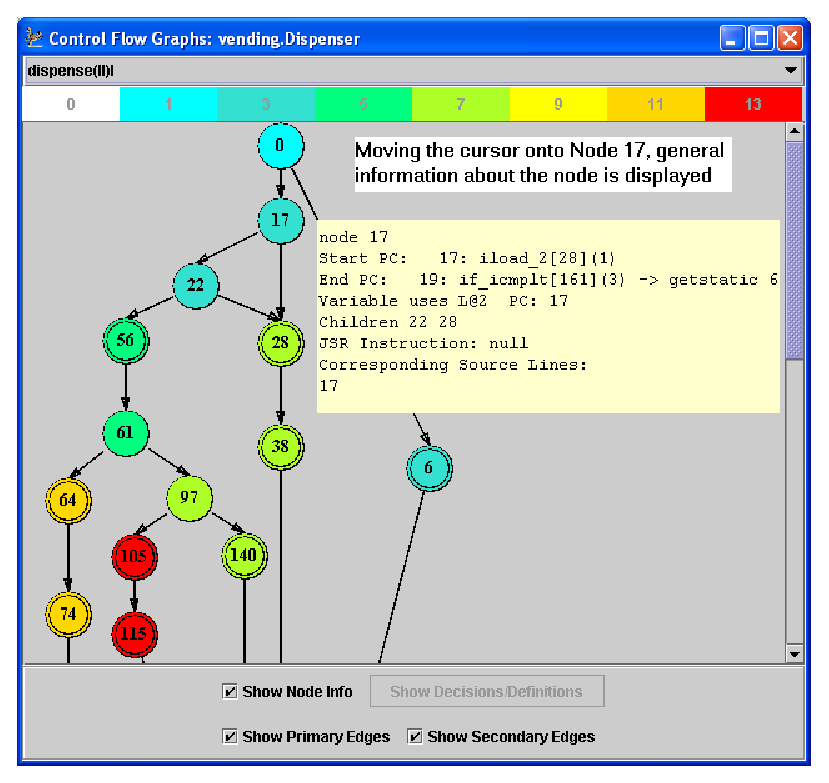
\includegraphics[height=0.35\textheight]{fig/dispenser-dug-edited.eps}
\caption{\label{fig:dispenser-dug} \pk{Dispenser.dispenser}
method: \DUG prioritized \wrt \pk{All-Pri-Nodes} criterion.}
\end{center}
\end{figure}


\begin{figure}[!ht]
\begin{center}
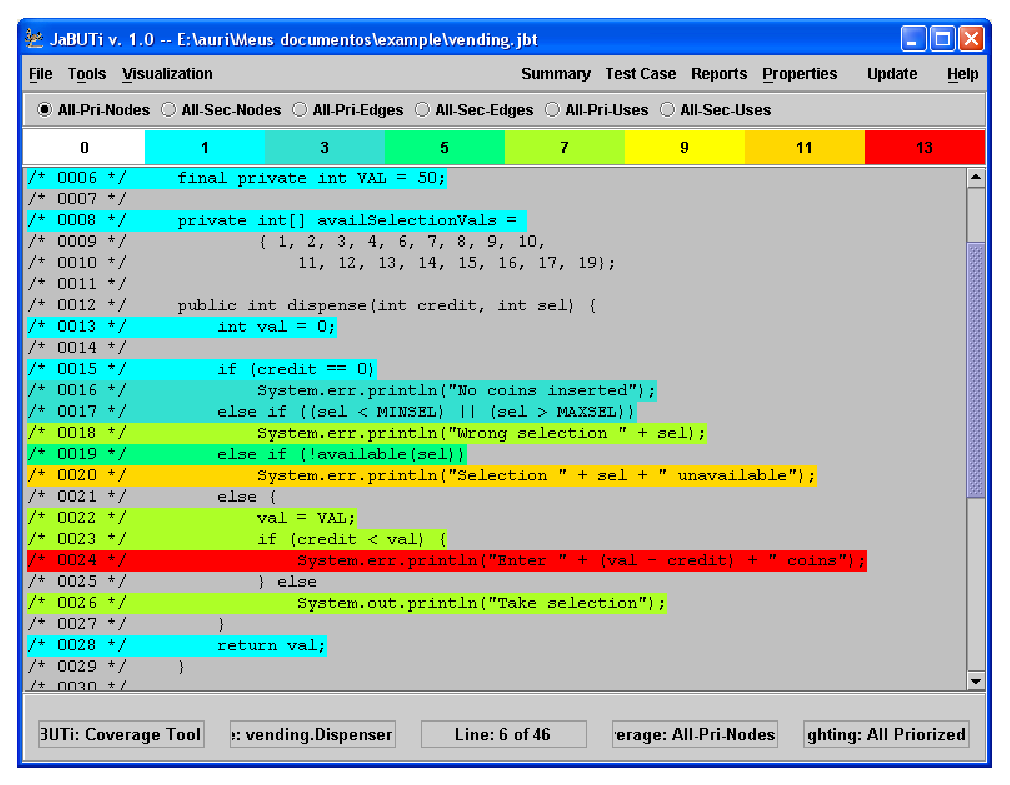
\includegraphics[height=0.40\textheight]{fig/dispenser-source.eps}
\caption{\label{fig:dispenser-source} \pk{Dispenser.dispenser}
method: source code prioritized \wrt \pk{All-Pri-Nodes}
criterion.}
\end{center}
\end{figure}


Considering the \DUG presented in Figure~\ref{fig:dispenser-dug},
it can be observed that there are two different types of nodes,
represented by single and double line circles. As described in
Section~\ref{sec:dependence}, double circles represent call nodes,
\ie, nodes where exists a method call to another method. This
nodes are identified since we intend to extend our tool to deal,
not only with intra-method testing criteria, but also with
inter-method testing criteria that requires the identification of
the relationship among methods. Bold circles, not visible in
Figure~\ref{fig:dispenser-dug}, represent exit nodes. Observe that
methods in Java can have more that one exit node due to the
exception-handling mechanism. All the other nodes are represented
as single line circles. We also have two different types of edges
to represent the ``normal'' control-flow (continuous line --
Primary Edges) and exception control-flow (dashed lines --
Secondary Edges). Figure~\ref{fig:dispenser-dug} does not contain
exception edges. Primary and secondary edges can be hidden by
deselecting the \pk{Show Primary} and \pk{Show Secondary Edges}
check box, respectively. The node information shown when the
cursor is moved onto the node, as illustrated in
Figure~\ref{fig:dispenser-dug}, can also be disabled by
deselecting the \pk{Show Node Info} check box.

\subsection{How the testing requirements are highlighted}

As can be observed above the main menu in
Figure~\ref{fig:dispenser-bytecode}, \toolname supports the
application of six structural testing criteria, as described in
Section~\ref{sec:criteria}: All-Pri-Nodes, All-Sec-Nodes,
All-Pri-Edges, All-Sec-Edges, All-Pri-Uses, and All-Sec-Uses.
Depending on which criterion is active, the bytecode, source code
or \DUG is colored in a different way.
Figures~\ref{fig:dispenser-bytecode}, \ref{fig:dispenser-dug},
and~\ref{fig:dispenser-source} show the color schema considering
the \pk{All-Pri-Nodes} criterion, which is the same as the
\pk{All-Sec-Nodes}, i.e., for these criteria, each requirement is
a node, therefore, since each node has its own weight, the
complete bytecode, source code or \DUG appears highlighted
according to the weight of each node.

Considering the \pk{All-Pri-Edges} and \pk{All-Sec-Edges}
criteria, their requirements (\DUG edges) are colored using a
2-layer approach. For \pk{All-Pri-Edges} criterion, only the nodes
with more than one out-going edge (decision nodes) are painted in
the first layer. For example, Figure~\ref{fig:decision-color}
shows part of the decision nodes of method
\pk{Dispenser.dispense()} and how they are painted in the first
layer. For each decision node, its weight is the maximum weight of
its branches. Suppose a decision node has two branches: one has a
weight of 2 and the other has a weight of 7. The weight of this
decision node is 7. This is the case of \DUG node 61, in our
example. A decision node has a zero weight if and only if all its
branches are covered. Such decisions are highlighted in white.
Observe that, in the bytecode view, only the last bytecode
instruction of a decision node is highlighted, not the entire node
as the \pk{All-Pri-Nodes} and the \pk{All-Sec-Nodes} criteria. For
example, \DUG decision node 22 goes from offset 22 to 25,
although, in the bytecode view, only bytecode instruction at
offset 25 is highlighted.

\begin{figure}[!ht]
\begin{center}
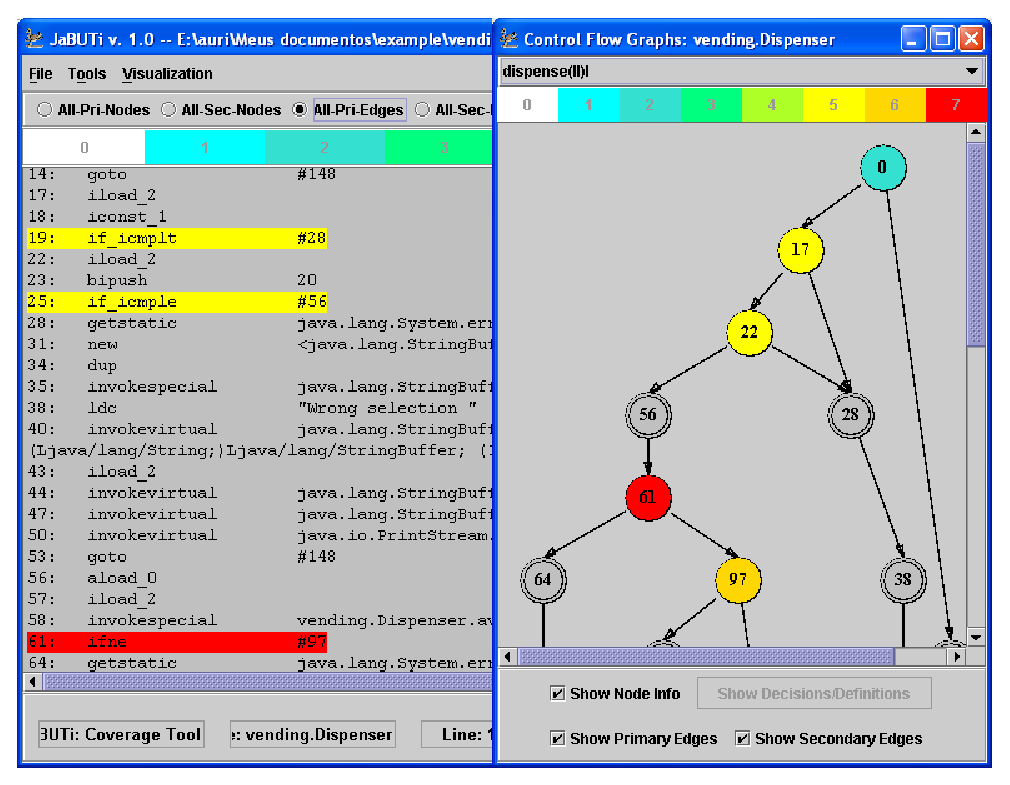
\includegraphics[height=0.40\textheight]{fig/decision-layer1.eps}
\caption{\label{fig:decision-color} Color schema for
\pk{All-Pri-Edges} criterion: first layer.}
\end{center}
\end{figure}


By clicking either in a colored bytecode instruction or in a \DUG
node, all destination nodes of the branches associated with the
selected decision node are highlighted and the decision node
itself changes to a different color. For example, by clicking on
the decision node with the highest weight (node 61 in the
example), its children (nodes 64 and 97) are highlighted in
different colors, considering their individual weights: node 64
has a weight of 7 (red) and node 97 has a weight of 2 (dark cyan),
as illustrated in Figure~\ref{fig:decision-color2}. Therefore, to
improve the coverage with respect to the \pk{All-Pri-Edges}
criterion, the tester should exercises first the edge
\edg{61}{64}, since it has the highest weight.

\begin{figure}[!ht]
\begin{center}
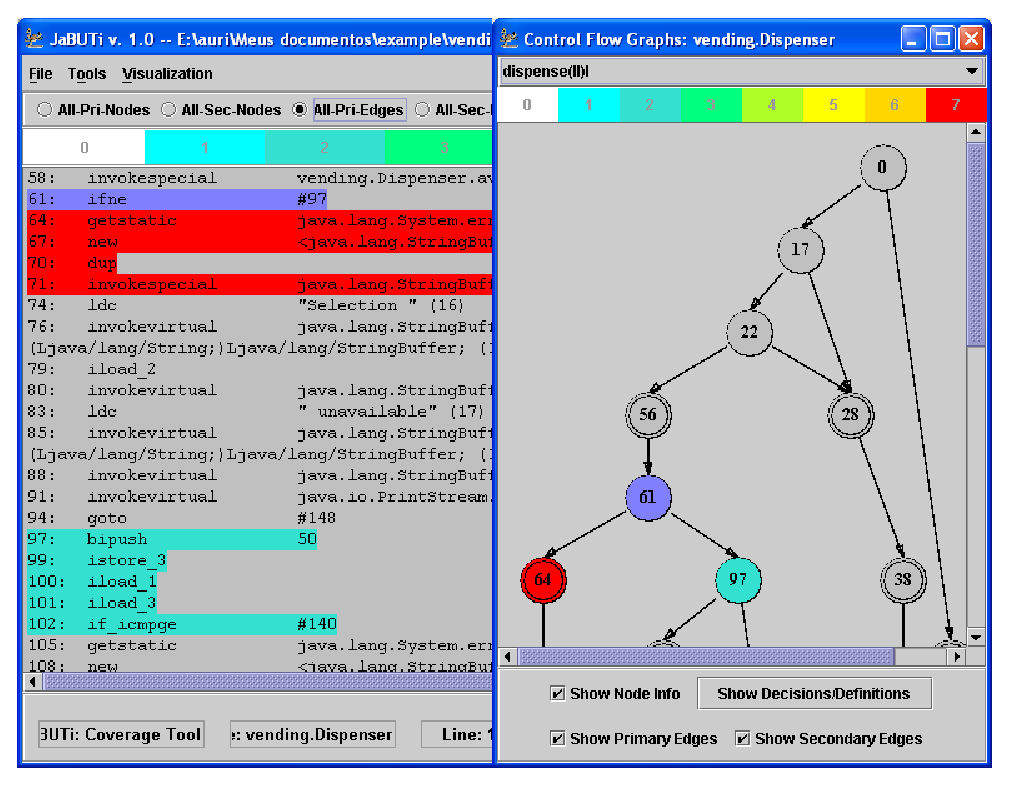
\includegraphics[height=0.40\textheight]{fig/decision-layer2.eps}
\caption{\label{fig:decision-color2} Color schema for
\pk{All-Pri-Edges} criterion: second layer.}
\end{center}
\end{figure}


\rev{Observe that, in case a given method has no decision node,
only the entry node is painted in the first layer and its child in
the second layer. In this case, edges criterion is equivalent to
nodes criterion, since, in a normal execution, once the entry node
is exercised, all the other nodes and edges are.}
Figure~\ref{fig:no-decision} illustrates how the \DUG of the
default constructor of the class \pk{VendingMachine}
(\pk{VendingMachine.init()}) is highlighted before
(Figure~\ref{fig:no-decision-1}) and after
(Figure~\ref{fig:no-decision-2}) the node selection.

\begin{figure}[!ht]
\begin{center}
\subfigure[]{\label{fig:no-decision-1}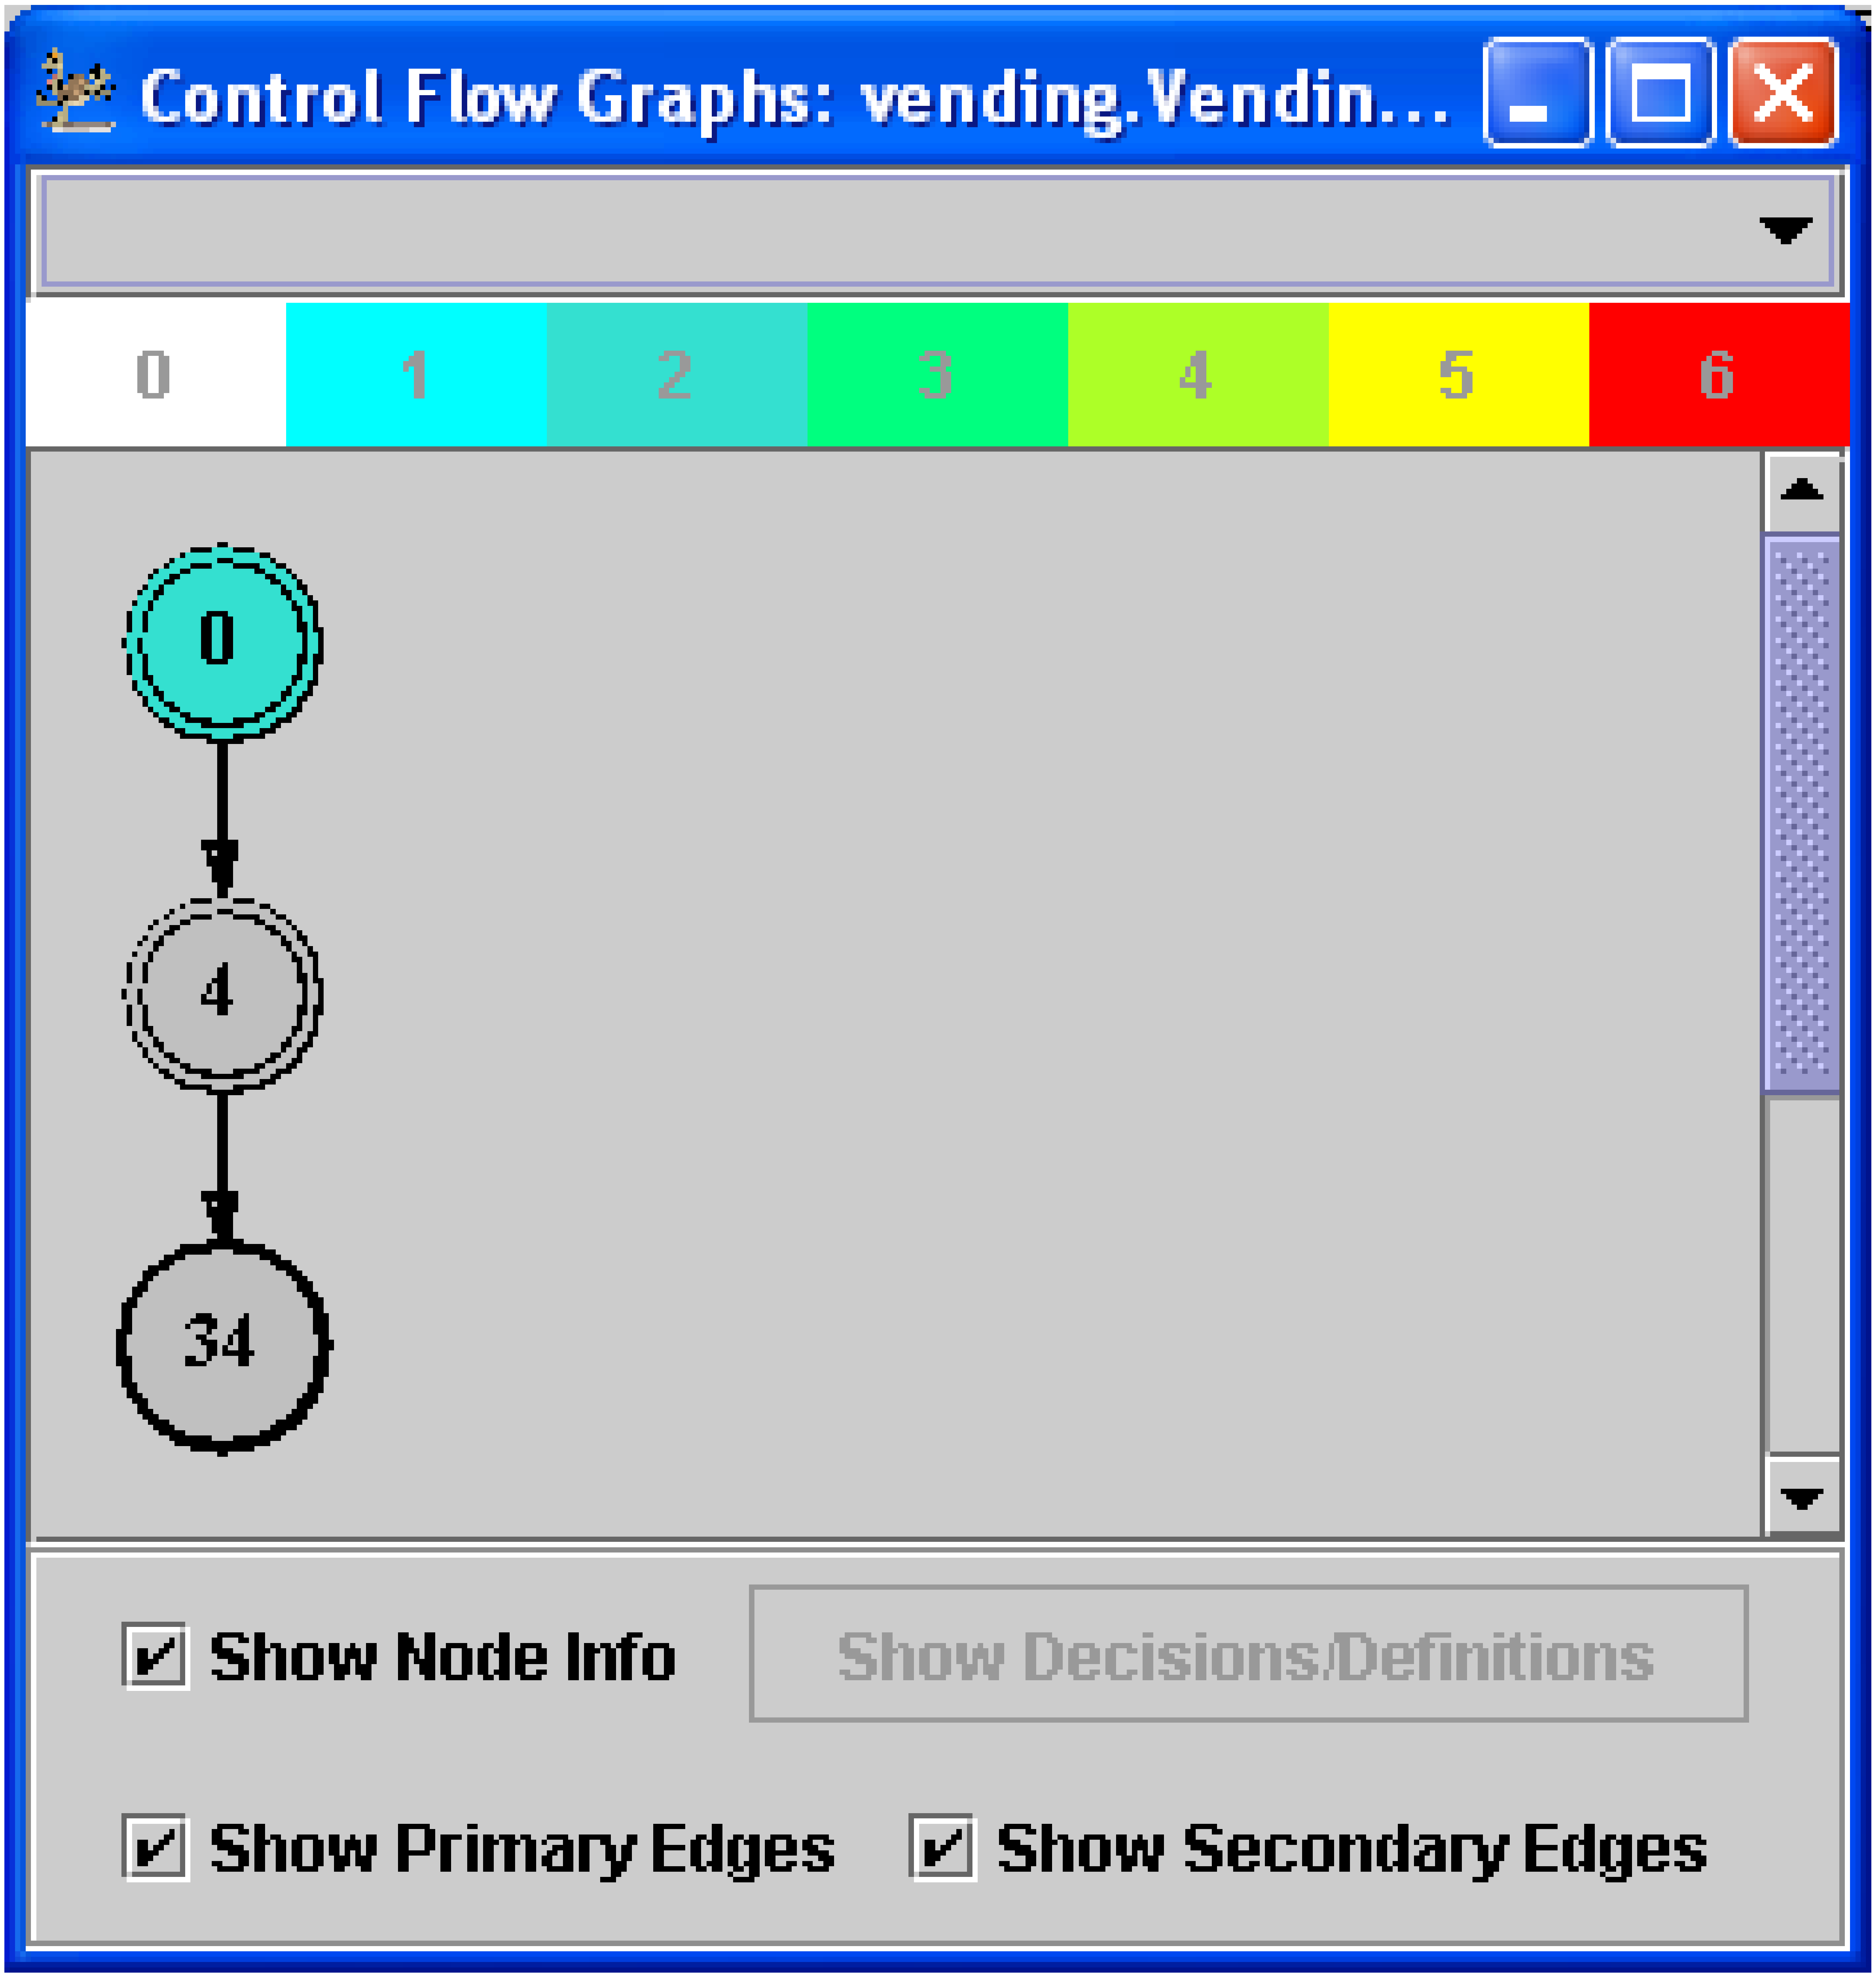
\includegraphics[width=0.45\textwidth]{fig/special-pri-edges-layer1.eps}}\qquad
\subfigure[]{\label{fig:no-decision-2}\includegraphics[width=0.45\textwidth]{fig/special-pri-edges-layer2.eps}}
\caption{Special case when no decision node is
found.}\label{fig:no-decision}
\end{center}
\end{figure}


For the \pk{All-Sec-Edges} criterion, the same approach is used.
In the first layer, all nodes with at least one secondary
out-going edge, instead of decision nodes, are highlighted. For
each such a node, its weight is the maximum weight of its branches
and a node with more that one secondary out-going edge is
considered covered (zero weight) if and only if all
exception-handler associated with such a node is covered.

Figure~\ref{fig:sec-edges-1} and~\ref{fig:sec-edges-2} shows the
first and the second layer of \pk{Dispenser.available()} method,
considering the \pk{All-Sec-Edges} criterion, respectively. In
this example, in the first layer, all highlighted nodes has the
same weigh (one) since it has only one valid exception-handler for
the entire method. In the bytecode view, only the last bytecode
instruction of each node is highlighted. For example, node 20 goes
from offset 20 to 26, therefore, bytecode instruction at offset 26
is highlighted. By clicking on such an instruction or on the \DUG
node 20, Figure~\ref{fig:sec-edges-2} shows the resultant color
schema of the second layer.

\begin{figure}[!ht]
\begin{center}
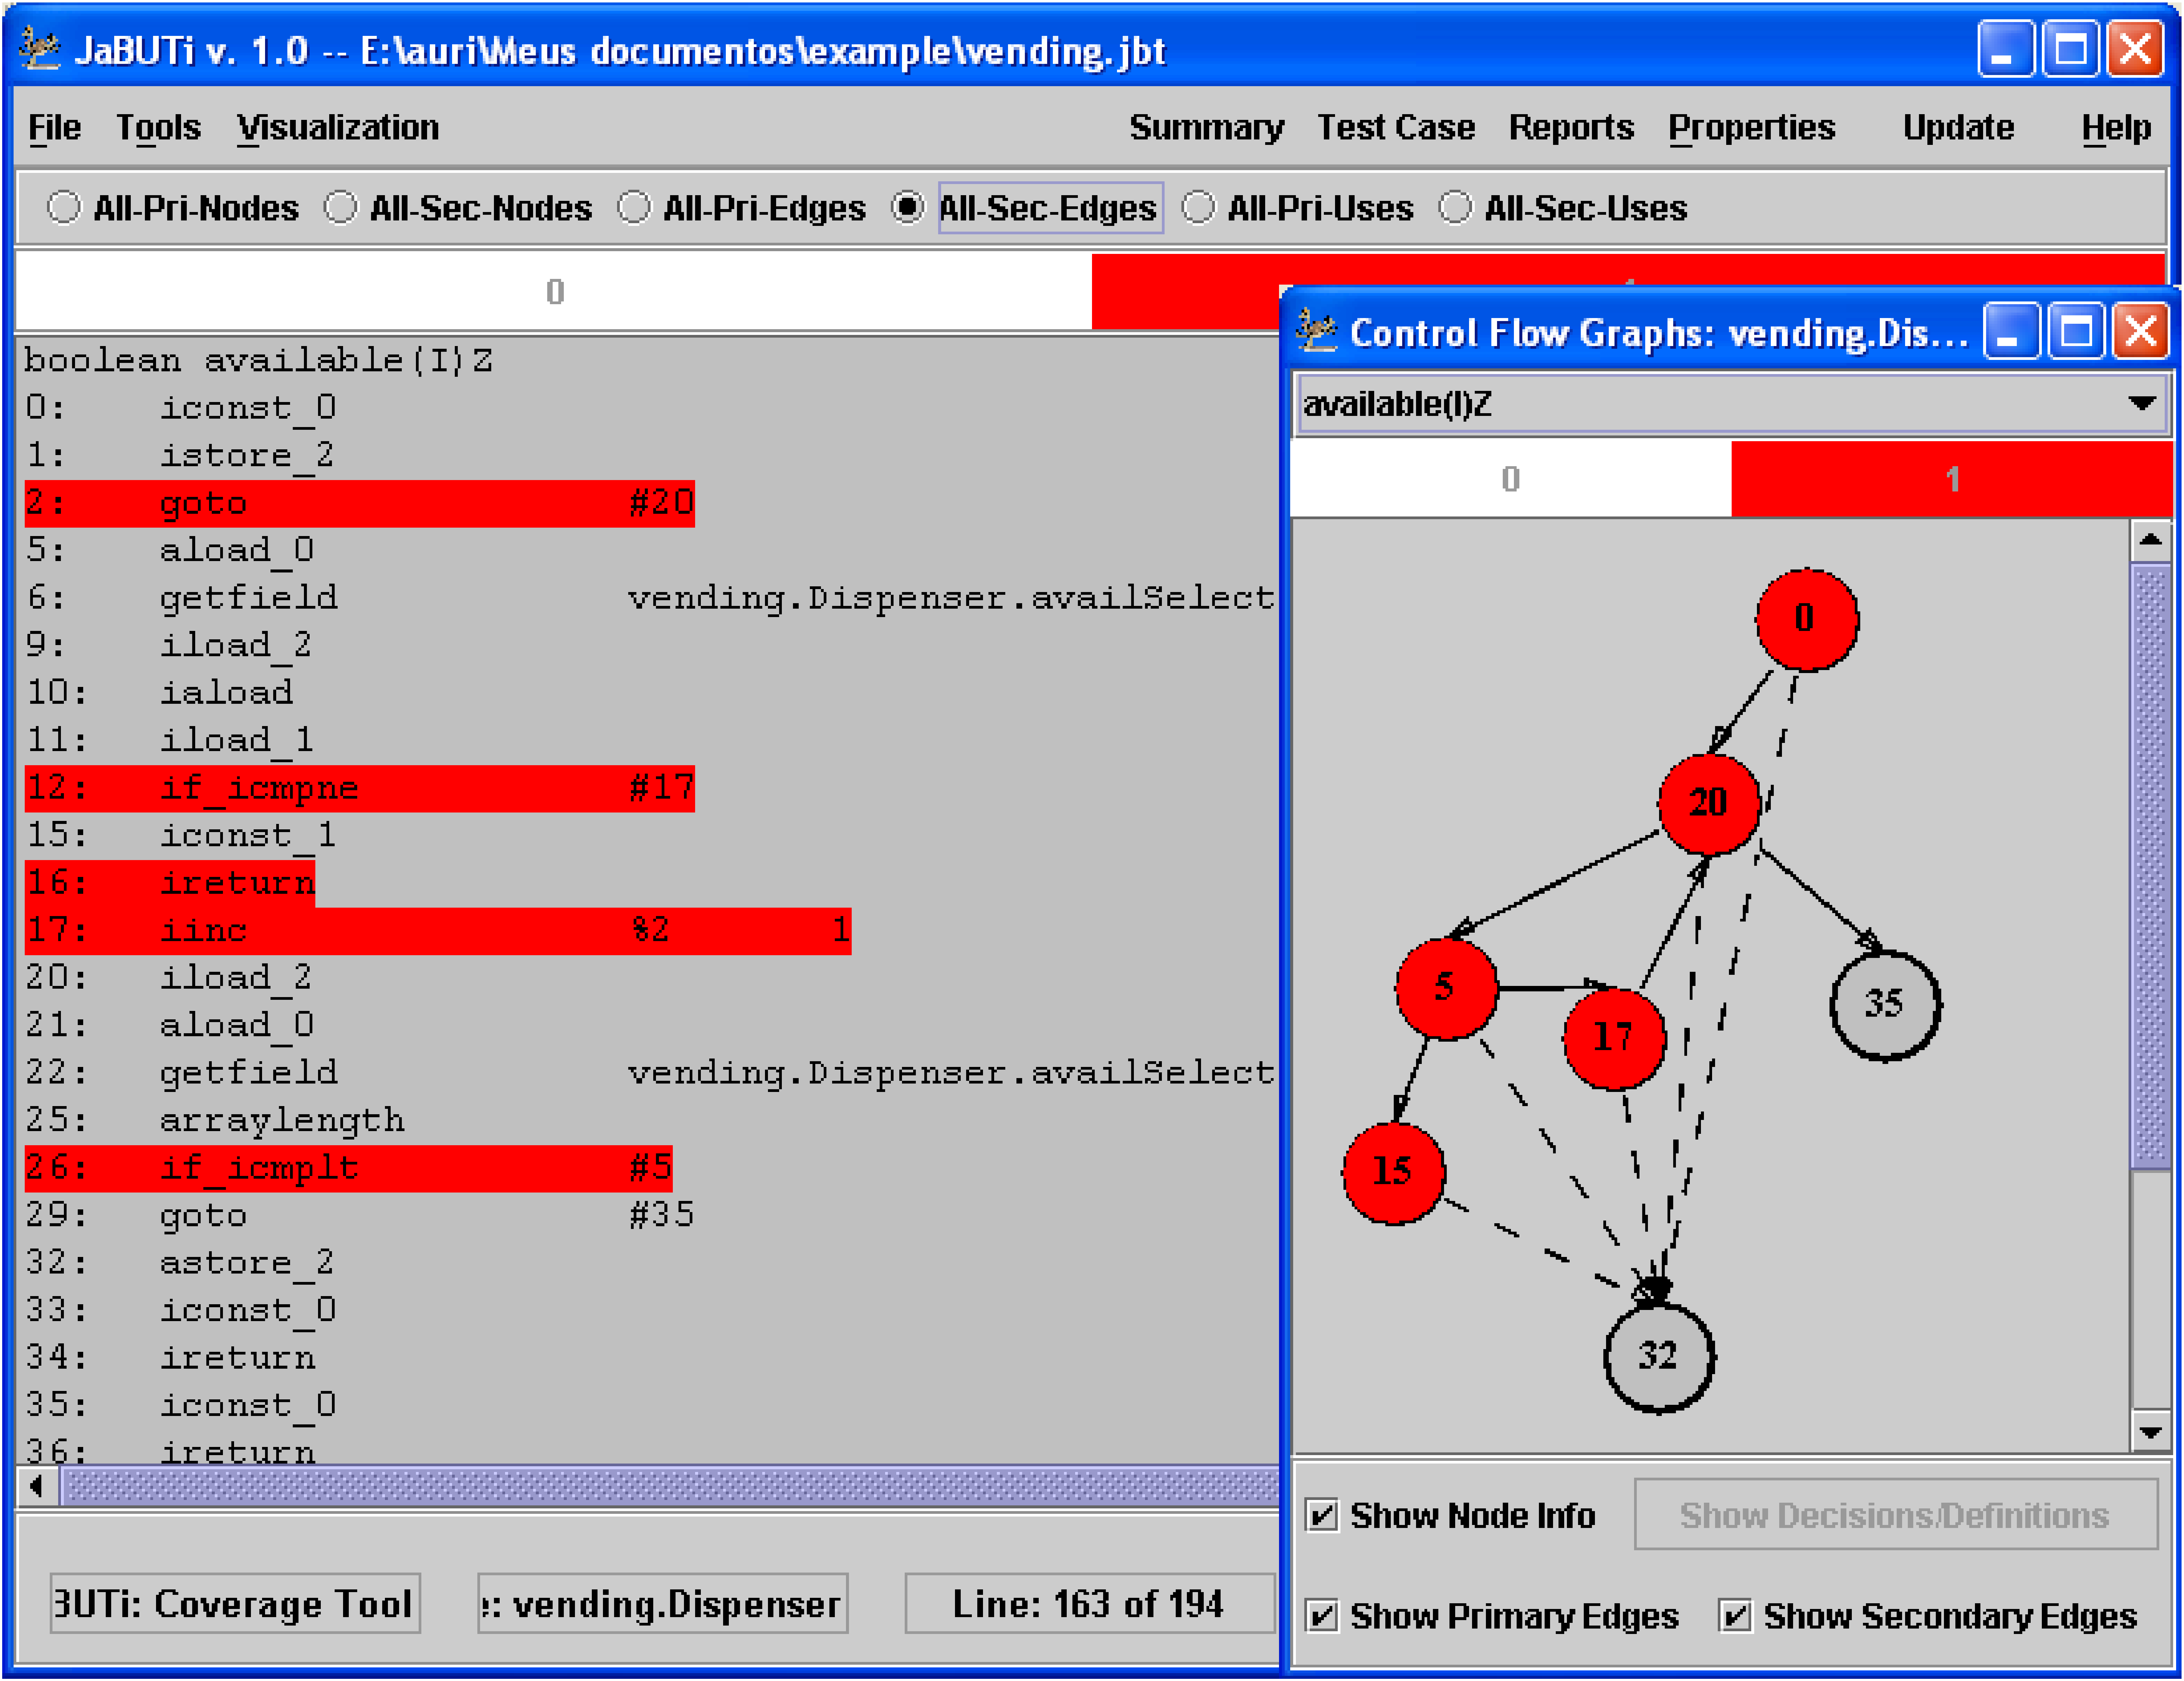
\includegraphics[height=0.40\textheight]{fig/sec-edges-layer1.eps}
\caption{\label{fig:sec-edges-1} Color schema for
\pk{All-Sec-Edges} criterion: first layer.}
\end{center}
\end{figure}


\begin{figure}[!ht]
\begin{center}
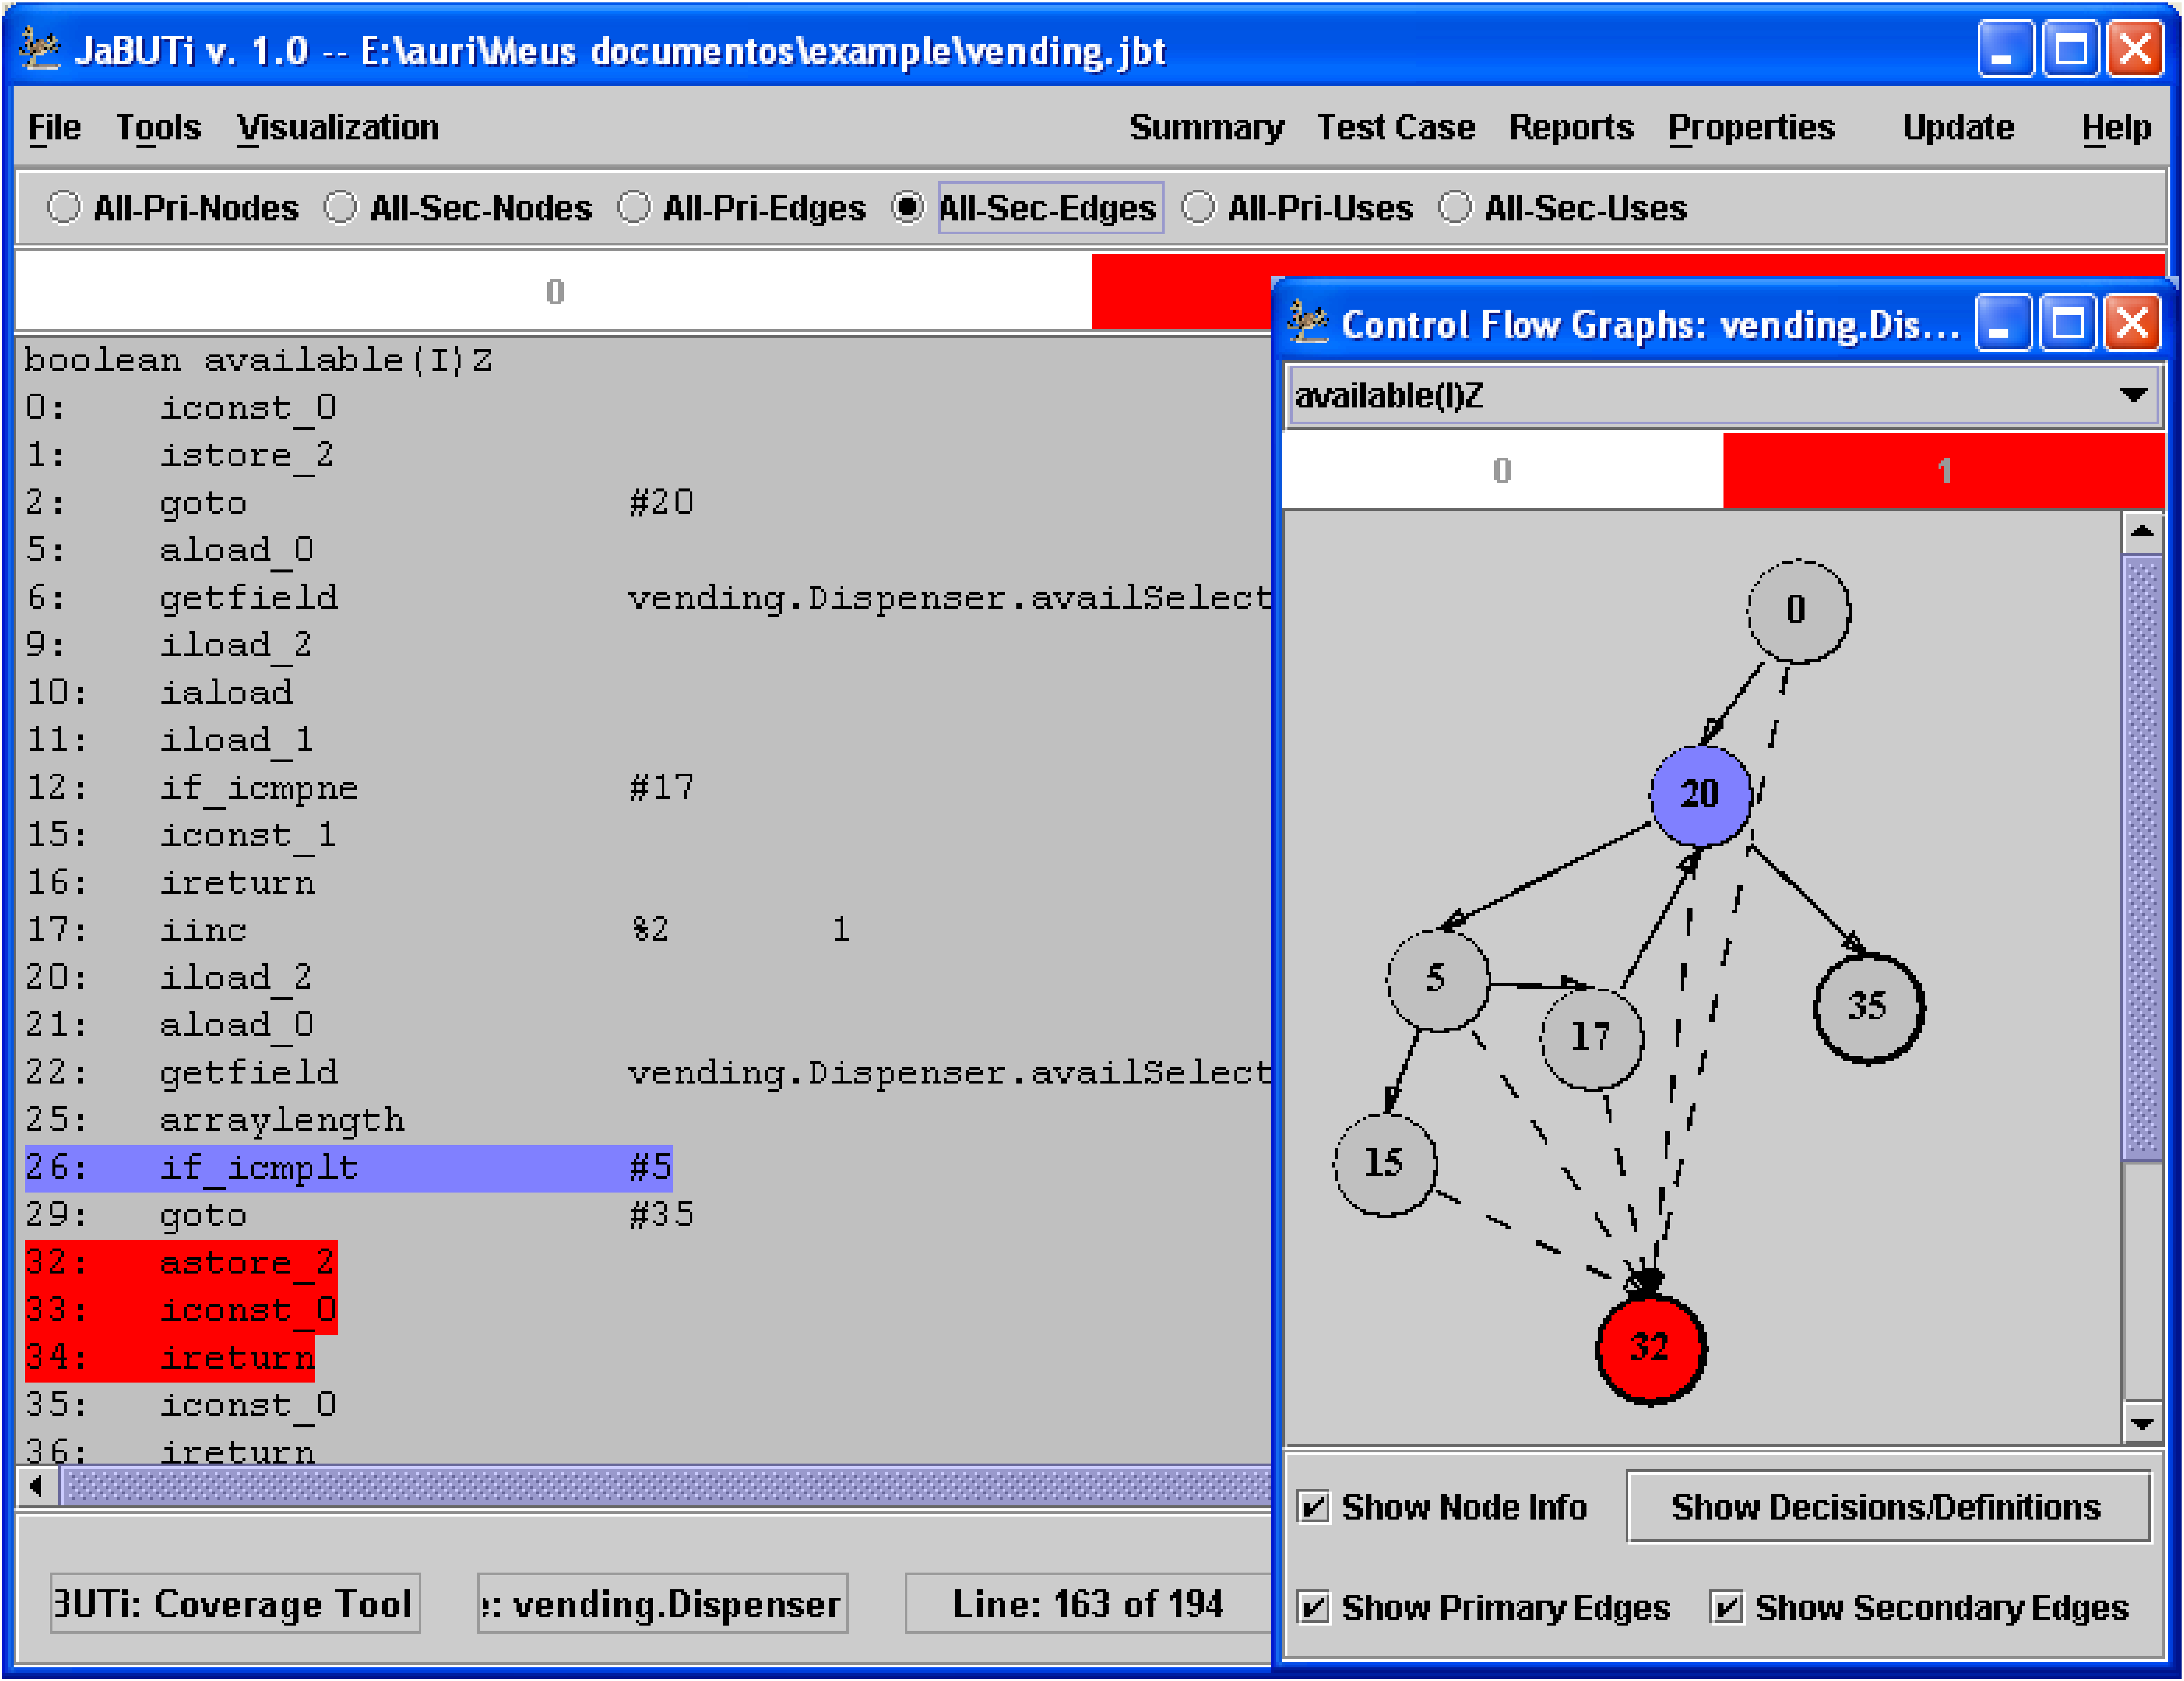
\includegraphics[height=0.40\textheight]{fig/sec-edges-layer2.eps}
\caption{\label{fig:sec-edges-2} Color schema for
\pk{All-Sec-Edges} criterion: second layer.}
\end{center}
\end{figure}


Similar to a decision and its branches are displayed, a 2-layer
representation is also used to display def-use associations for
the \pk{All-Pri-Uses} and \pk{All-Sec-Uses} criteria. The first
layer shows all the definitions which have at least one c-use or
p-use association. Clicking on a definition goes to the second
layer displaying all c-use and p-use associated with the selected
definition. For each definition, its weight is the maximum weight
of its c-uses or p-uses. For example, suppose a definition has
three def-use associations, one c-use and two p-uses, and the
weights of these associations are 5, 3 and 7, respectively. The
weight of this definition is 7. A definition has a zero weight if
and only if all its c-uses and p-uses are covered. Such
definitions are displayed with a white background.

Since even in the bytecode, more than one variable may be defined
in the same offset, if desired, by clicking with the right mouse
button over a definition point (bytecode offset, source code line
or \DUG node), a pop-up menu is opened showing all the variables
defined in that point such that it is possible to choose which
variable definition to select. For example,
Figure~\ref{fig:uses-color} shows the set of defined variables at
bytecode offset 0 that is part of the \DUG node 0. Observe that in
the \DUG node 0 there is one additional variable definition
because \pk{L@3 (val)} is defined at bytecode offset 1 that also
belongs to \DUG node 0. When a definition point is clicked with
the left mouse button the definition with the highest weight is
considered selected. If all of then have the same weight, the
first is selected. In our example, supposing that \pk{L@1
(credit)} is selected (the definition with the highest weight),
Figure~\ref{fig:uses-color2} shows some of its uses (p-uses in
this case) with the corresponding weight.

\begin{figure}[!ht]
\begin{center}

\includegraphics[height=0.40\textheight]{fig/pri-uses-layer1.eps}
\caption{\label{fig:uses-color} Color schema for \pk{All-Pri-Uses}
criterion: first layer.}
\end{center}
\end{figure}


\begin{figure}[!ht]
\begin{center}

\includegraphics[height=0.40\textheight]{fig/pri-uses-layer2.eps}
\caption{\label{fig:uses-color2} Color schema for
\pk{All-Pri-Uses} criterion: second layer.}
\end{center}
\end{figure}


It is important to observe that the weights provided by the tool
may be seen as hints for the tester to facilitate the generation
of test cases, such that a higher coverage can be obtained with
fewer test cases. Since the prioritization does not consider the
criticality of a given part of the code, if desired, the tester
may choose a different part of the code to be tested first based
on his/her knowledge about the application, even if such a part
has a lower weight than other parts of the code. After the
critical parts have to be tested, additional test cases can be
developed considering the hints.

\subsection{How to generate testing reports}

To evaluate the coverage obtained, the tool provides personalized
tabled style testing reports that can be accessed from the
\pk{Summary} and \pk{Test Case} menus. Any tabled style report can
be saved as a HTML file by accessing \pk{Reports $\rightarrow$
Summary to HTML} menu option. The tool provides reports \wrt each
testing criterion (\pk{Summary $\rightarrow$ By Criterion}), \wrt
each class file (\pk{Summary $\rightarrow$ By Class}) and \wrt
each method (\pk{Summary $\rightarrow$ By Method}).
Figures~\ref{fig:initial-summary-criterion},
\ref{fig:initial-summary-class},
and~\ref{fig:initial-summary-method} show each one of these
reports, respectively, considering that no test case have been
executed.

\begin{figure}[!ht]
\begin{center}
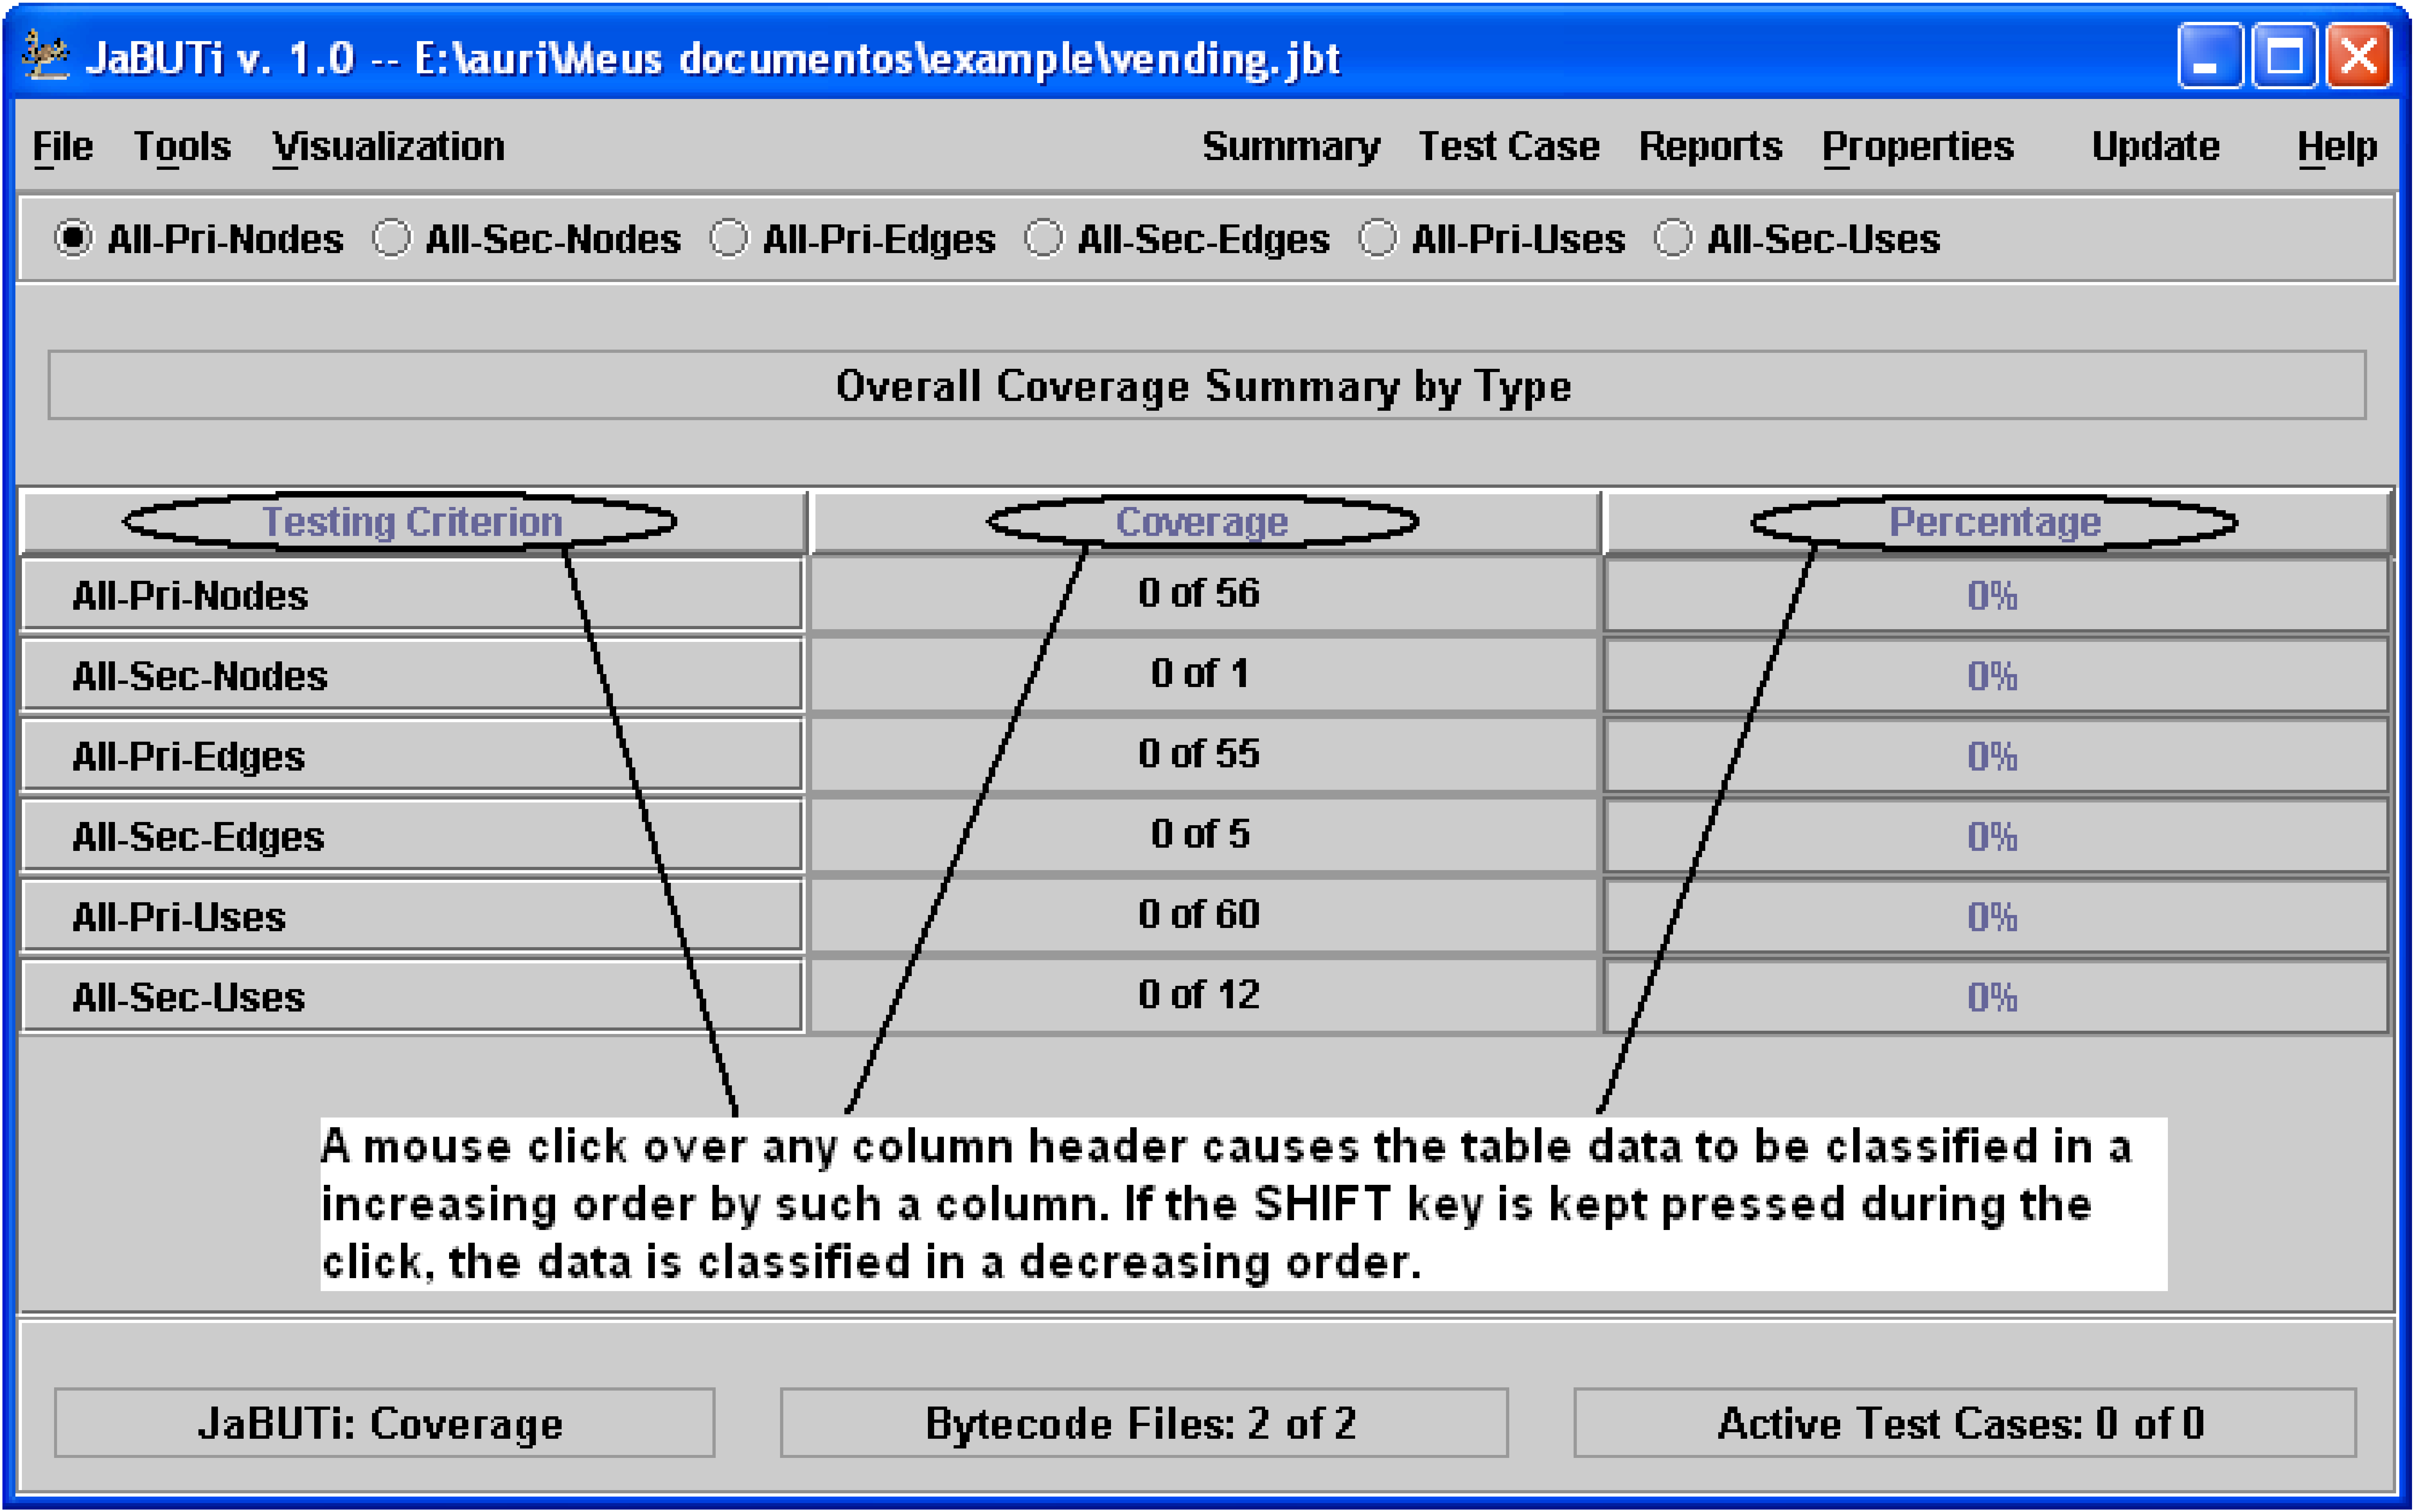
\includegraphics[width=0.70\textwidth]{fig/summary-by-criterion-initial-edited.eps}
\caption{\label{fig:initial-summary-criterion} Initial summary
information per testing criterion.}
\end{center}
\end{figure}


For example, in Figures~\ref{fig:initial-summary-criterion} it is
possible to evaluate the number of required elements by criterion
that were generated for the entire project, i.e., classes
\pk{VendingMachine} and \pk{Dispenser}. The individual information
per class file can be obtained by generating the summary report by
class (Figures~\ref{fig:initial-summary-class}).

When showing the summary by class or by method, the tester can
choose, among the available testing criteria, which one he/she
wants to evaluate.
Figures~\ref{fig:initial-summary-class-pri-nodes},
\ref{fig:initial-summary-class-pri-edges},
and~\ref{fig:initial-summary-class-pri-uses} illustrate the
summary per individual class \wrt the \pk{All-Pri-Nodes},
\pk{All-Pri-Edges}, and \pk{All-Pri-Uses} criteria, respectively.
Considering the summary by class and by method, by clicking on the
class file name or in the method name, the corresponding bytecode
is highlighted and displayed considering the weight \wrt the
selected criterion.

As commented in Figures~\ref{fig:initial-summary-criterion},
double-clicking on the desired column header, any tabled report
generated by \toolname is classified in an increasing order,
considering the clicked column header. A double-click with the
\pk{SHIFT} key pressed causes the table data to be sorted in a
decreasing order.

Using these summary reports the tester can evaluate the current
coverage of each class under testing with different granularity
and decides whether a given class requires additional testing \wrt
six different intra-method testing criteria.
Section~\ref{sec:testcase} illustrates how to include test cases
and how to generate testing reports by test case and by test case
paths.

\begin{figure}[!ht]
\begin{center}
\subfigure[]{\label{fig:initial-summary-class-pri-nodes}
\includegraphics[width=0.70\textwidth]{fig/summary-by-class-pri-nodes-edited.eps}}

\subfigure[]{\label{fig:initial-summary-class-pri-edges}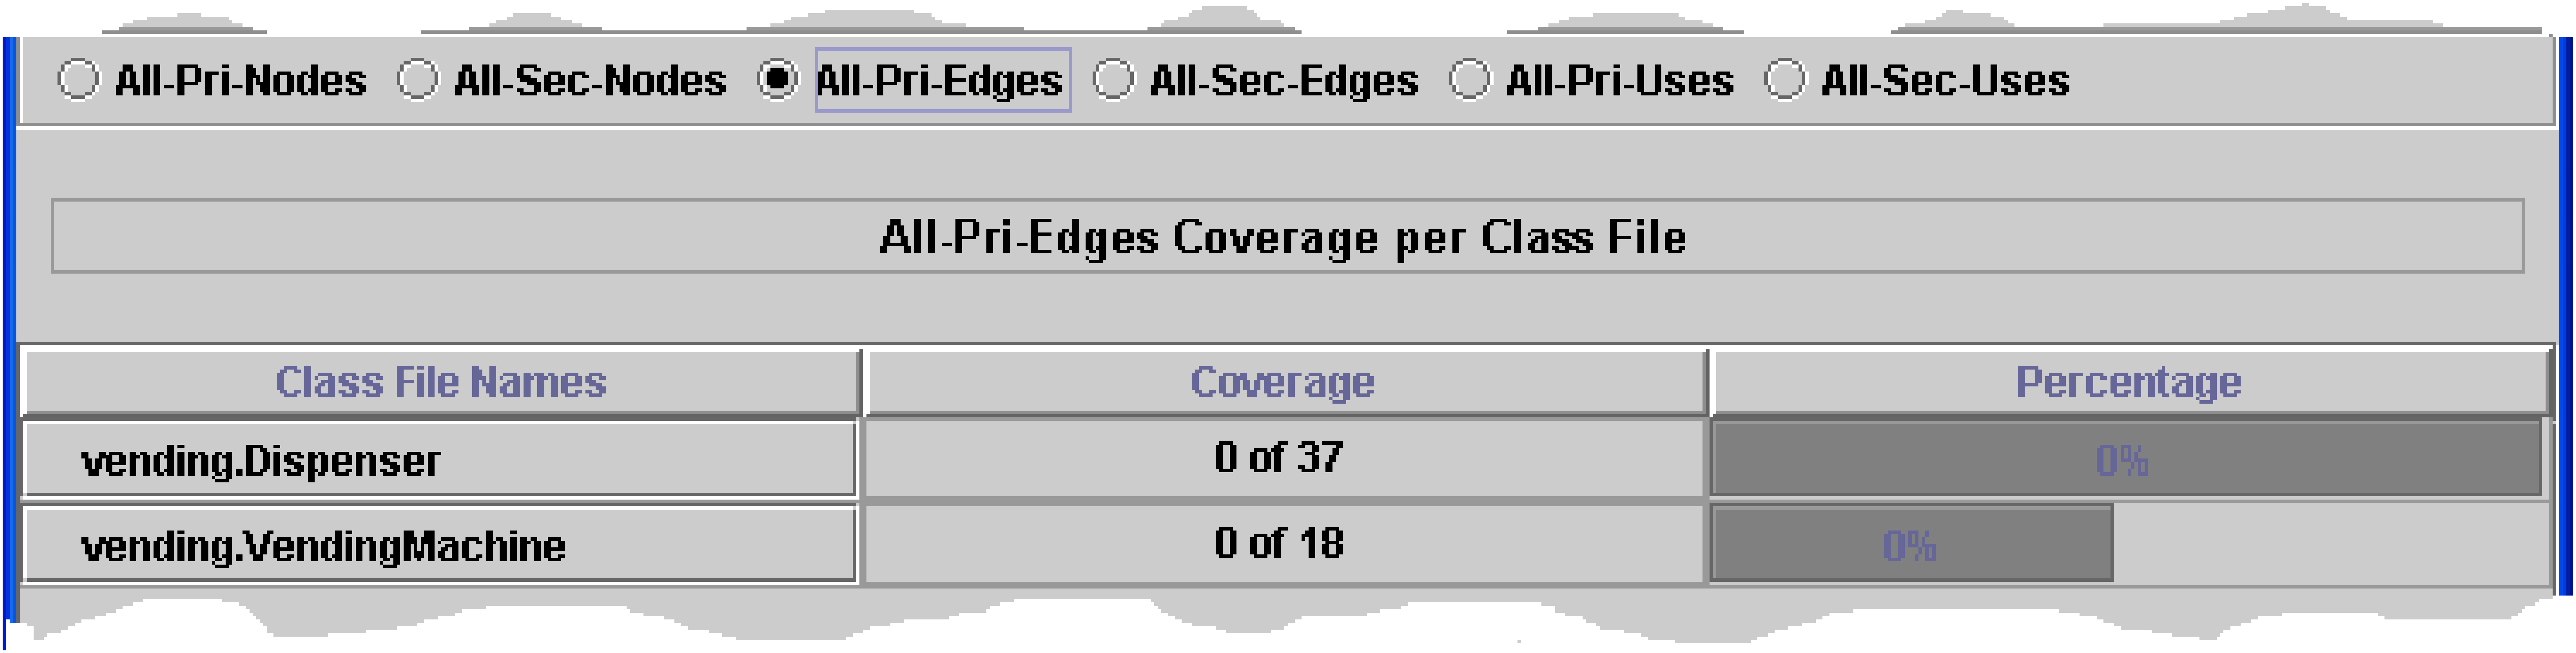
\includegraphics[width=0.70\textwidth]{fig/summary-by-class-pri-edges-edited.eps}}

\subfigure[]{\label{fig:initial-summary-class-pri-uses}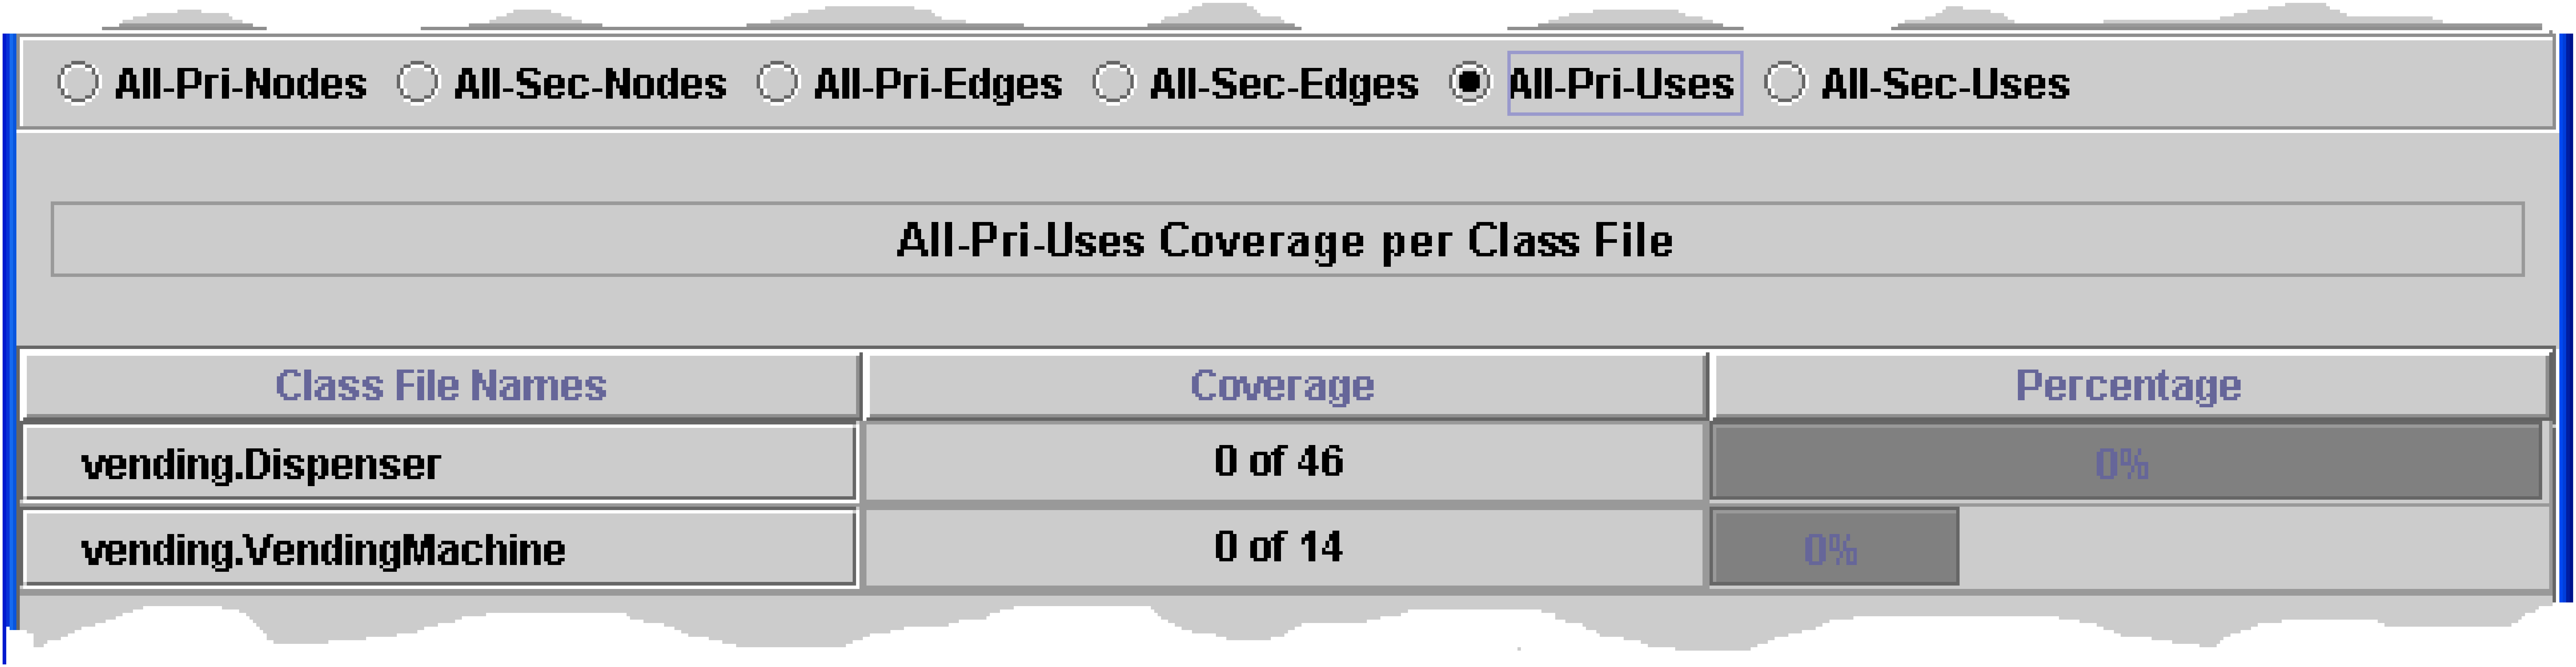
\includegraphics[width=0.70\textwidth]{fig/summary-by-class-pri-uses-edited.eps}}

\caption{Initial summary per class file: (a) \pk{All-Pri-Nodes}
criterion, (b) \pk{All-Pri-Edges} criterion, and (c)
\pk{All-Pri-Uses} criterion.}\label{fig:initial-summary-class}
\end{center}
\end{figure}


\begin{figure}[!ht]
\begin{center}
\includegraphics[width=0.70\textwidth]{fig/summary-by-method-initial.eps}
\caption{\label{fig:initial-summary-method} Initial summary
information per method: \pk{All-Pri-Nodes} criterion.}
\end{center}
\end{figure}


\afterpage{\clearpage}
\newpage

\subsection{How to generate an HTML version of a \toolname
report}

As mentioned above, any kind of tabled report presented in
\toolname's graphical interface can be saved as an HTML file
through the \pk{Reports $\rightarrow$ Summary to HTML} menu
option. For example, Figure~\ref{fig:summary-to-html} shows how to
create a \pk{summary-by-criterion.html} file, corresponding to the
current \toolname screen. Figure~\ref{fig:html-file} illustrates
the generated HTML file in a browser window. In this way the
tester can collect and save different testing report showing the
evolution of the testing activity.

\begin{figure}[!ht]
\begin{center}
\subfigure[]{\label{fig:summary-to-html}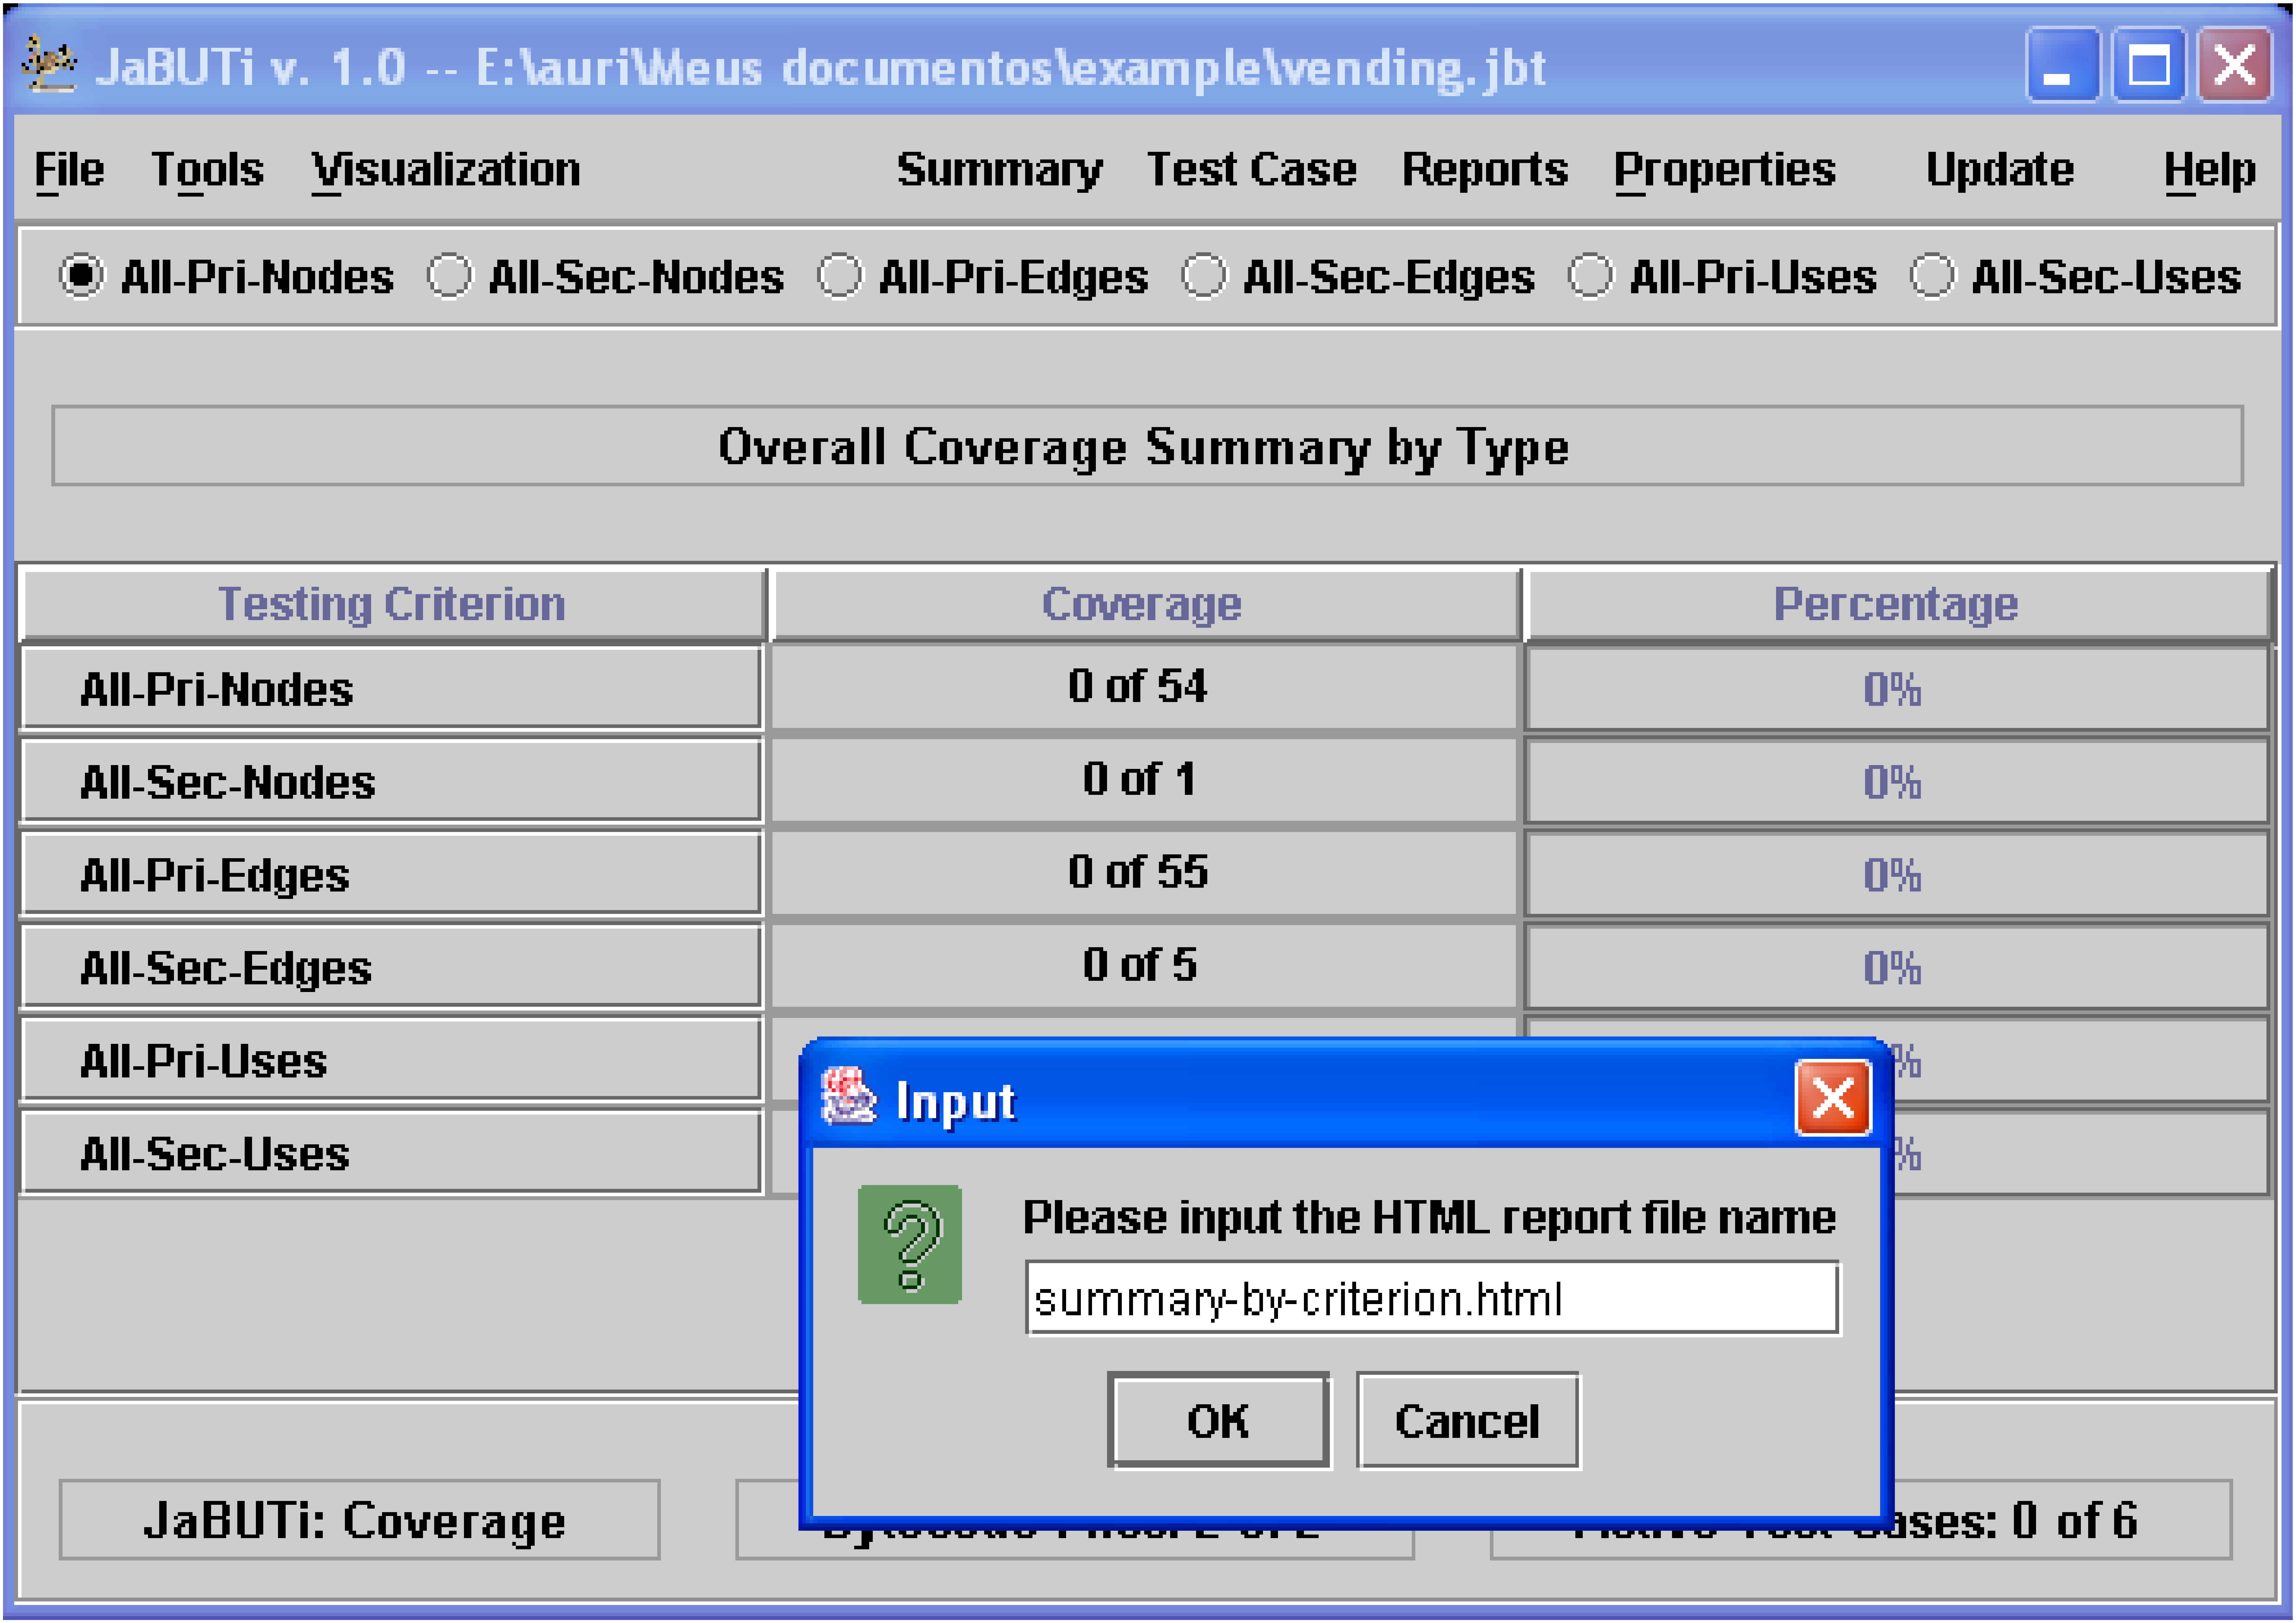
\includegraphics[width=0.45\textwidth]{fig/summary-to-html.eps}}\qquad
\subfigure[]{\label{fig:html-file}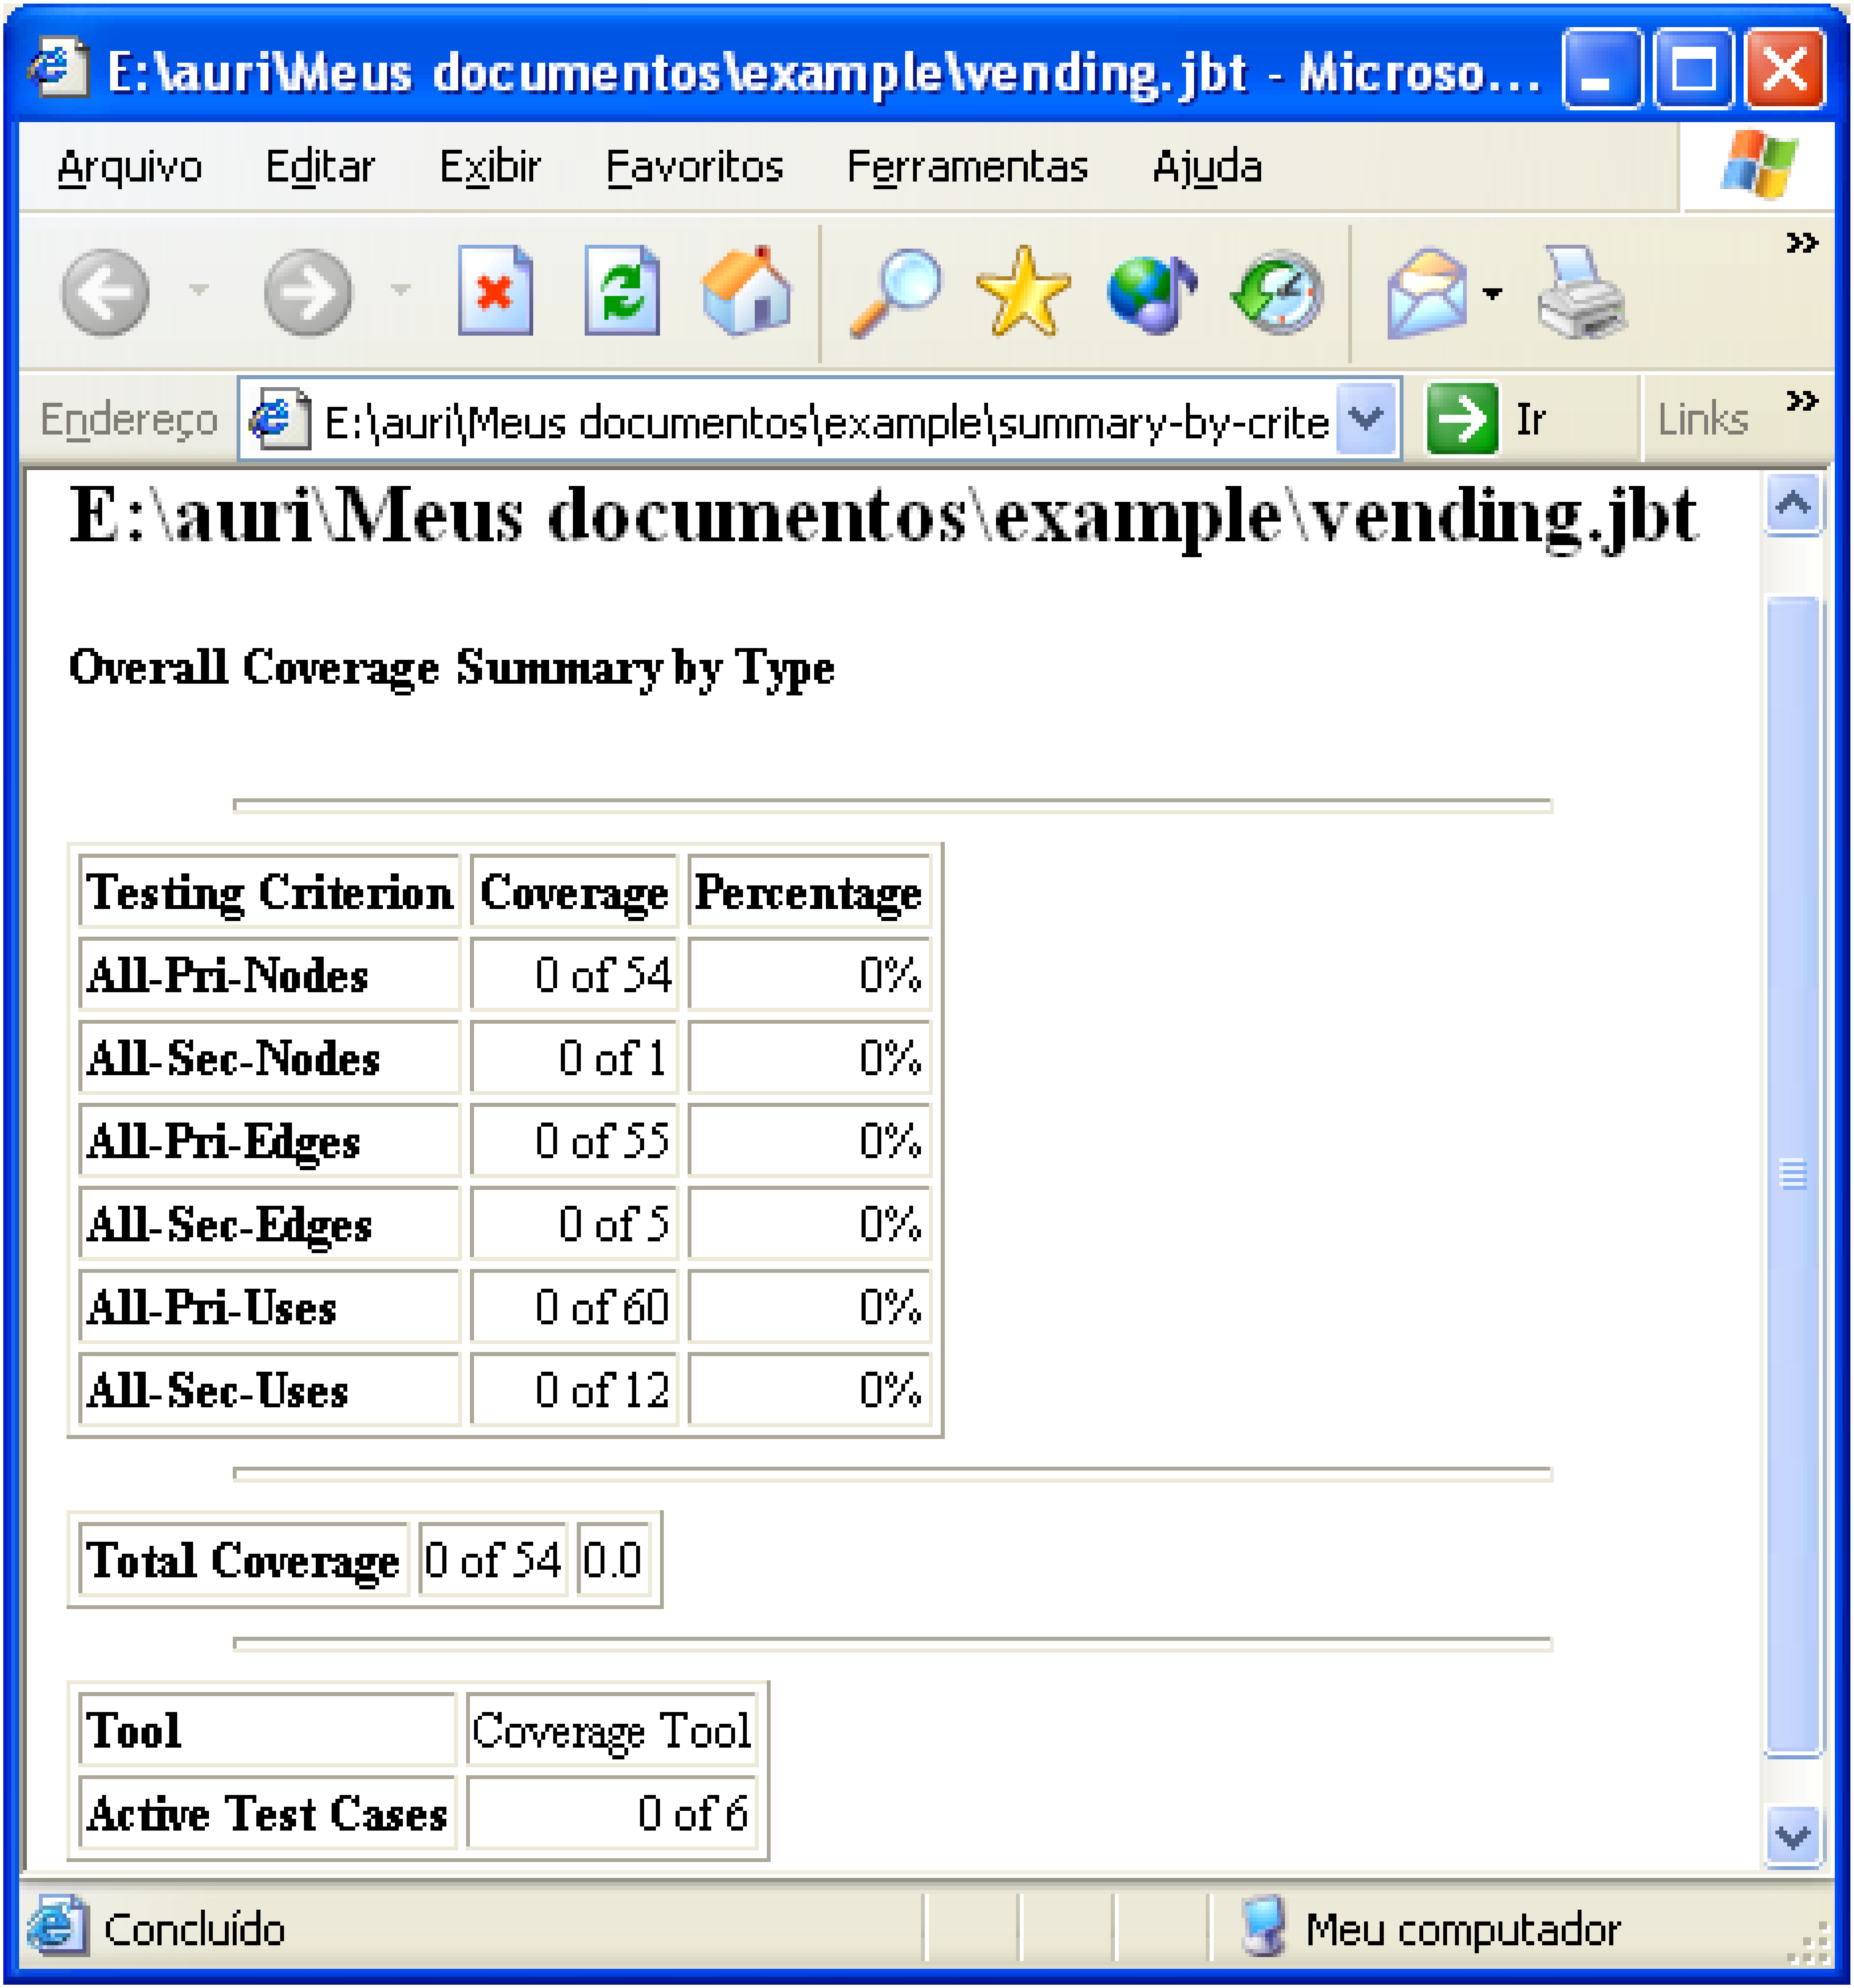
\includegraphics[width=0.45\textwidth]{fig/summary-by-criterion-html.eps}}
\caption{Example of an HTML report generated by
\toolname.}\label{fig:html-report}
\end{center}
\end{figure}


A different kind of report can be generated through the
\pk{Reports $\rightarrow$ Custom Report} menu option. By selecting
this option, a dialog windows, as illustrated in
Figure~\ref{fig:custom-html}, appears and the tester can choose
the level of information that will be saved in a HTML file.
Observe that to save information at method level it is also
required to save information about the class and project level,
since the information is saved hierarchically. Part of a complete
report for the entire project is presented in
Figure~\ref{fig:html-file2}.

\begin{figure}[!ht]
\begin{center}
\subfigure[]{\label{fig:custom-html}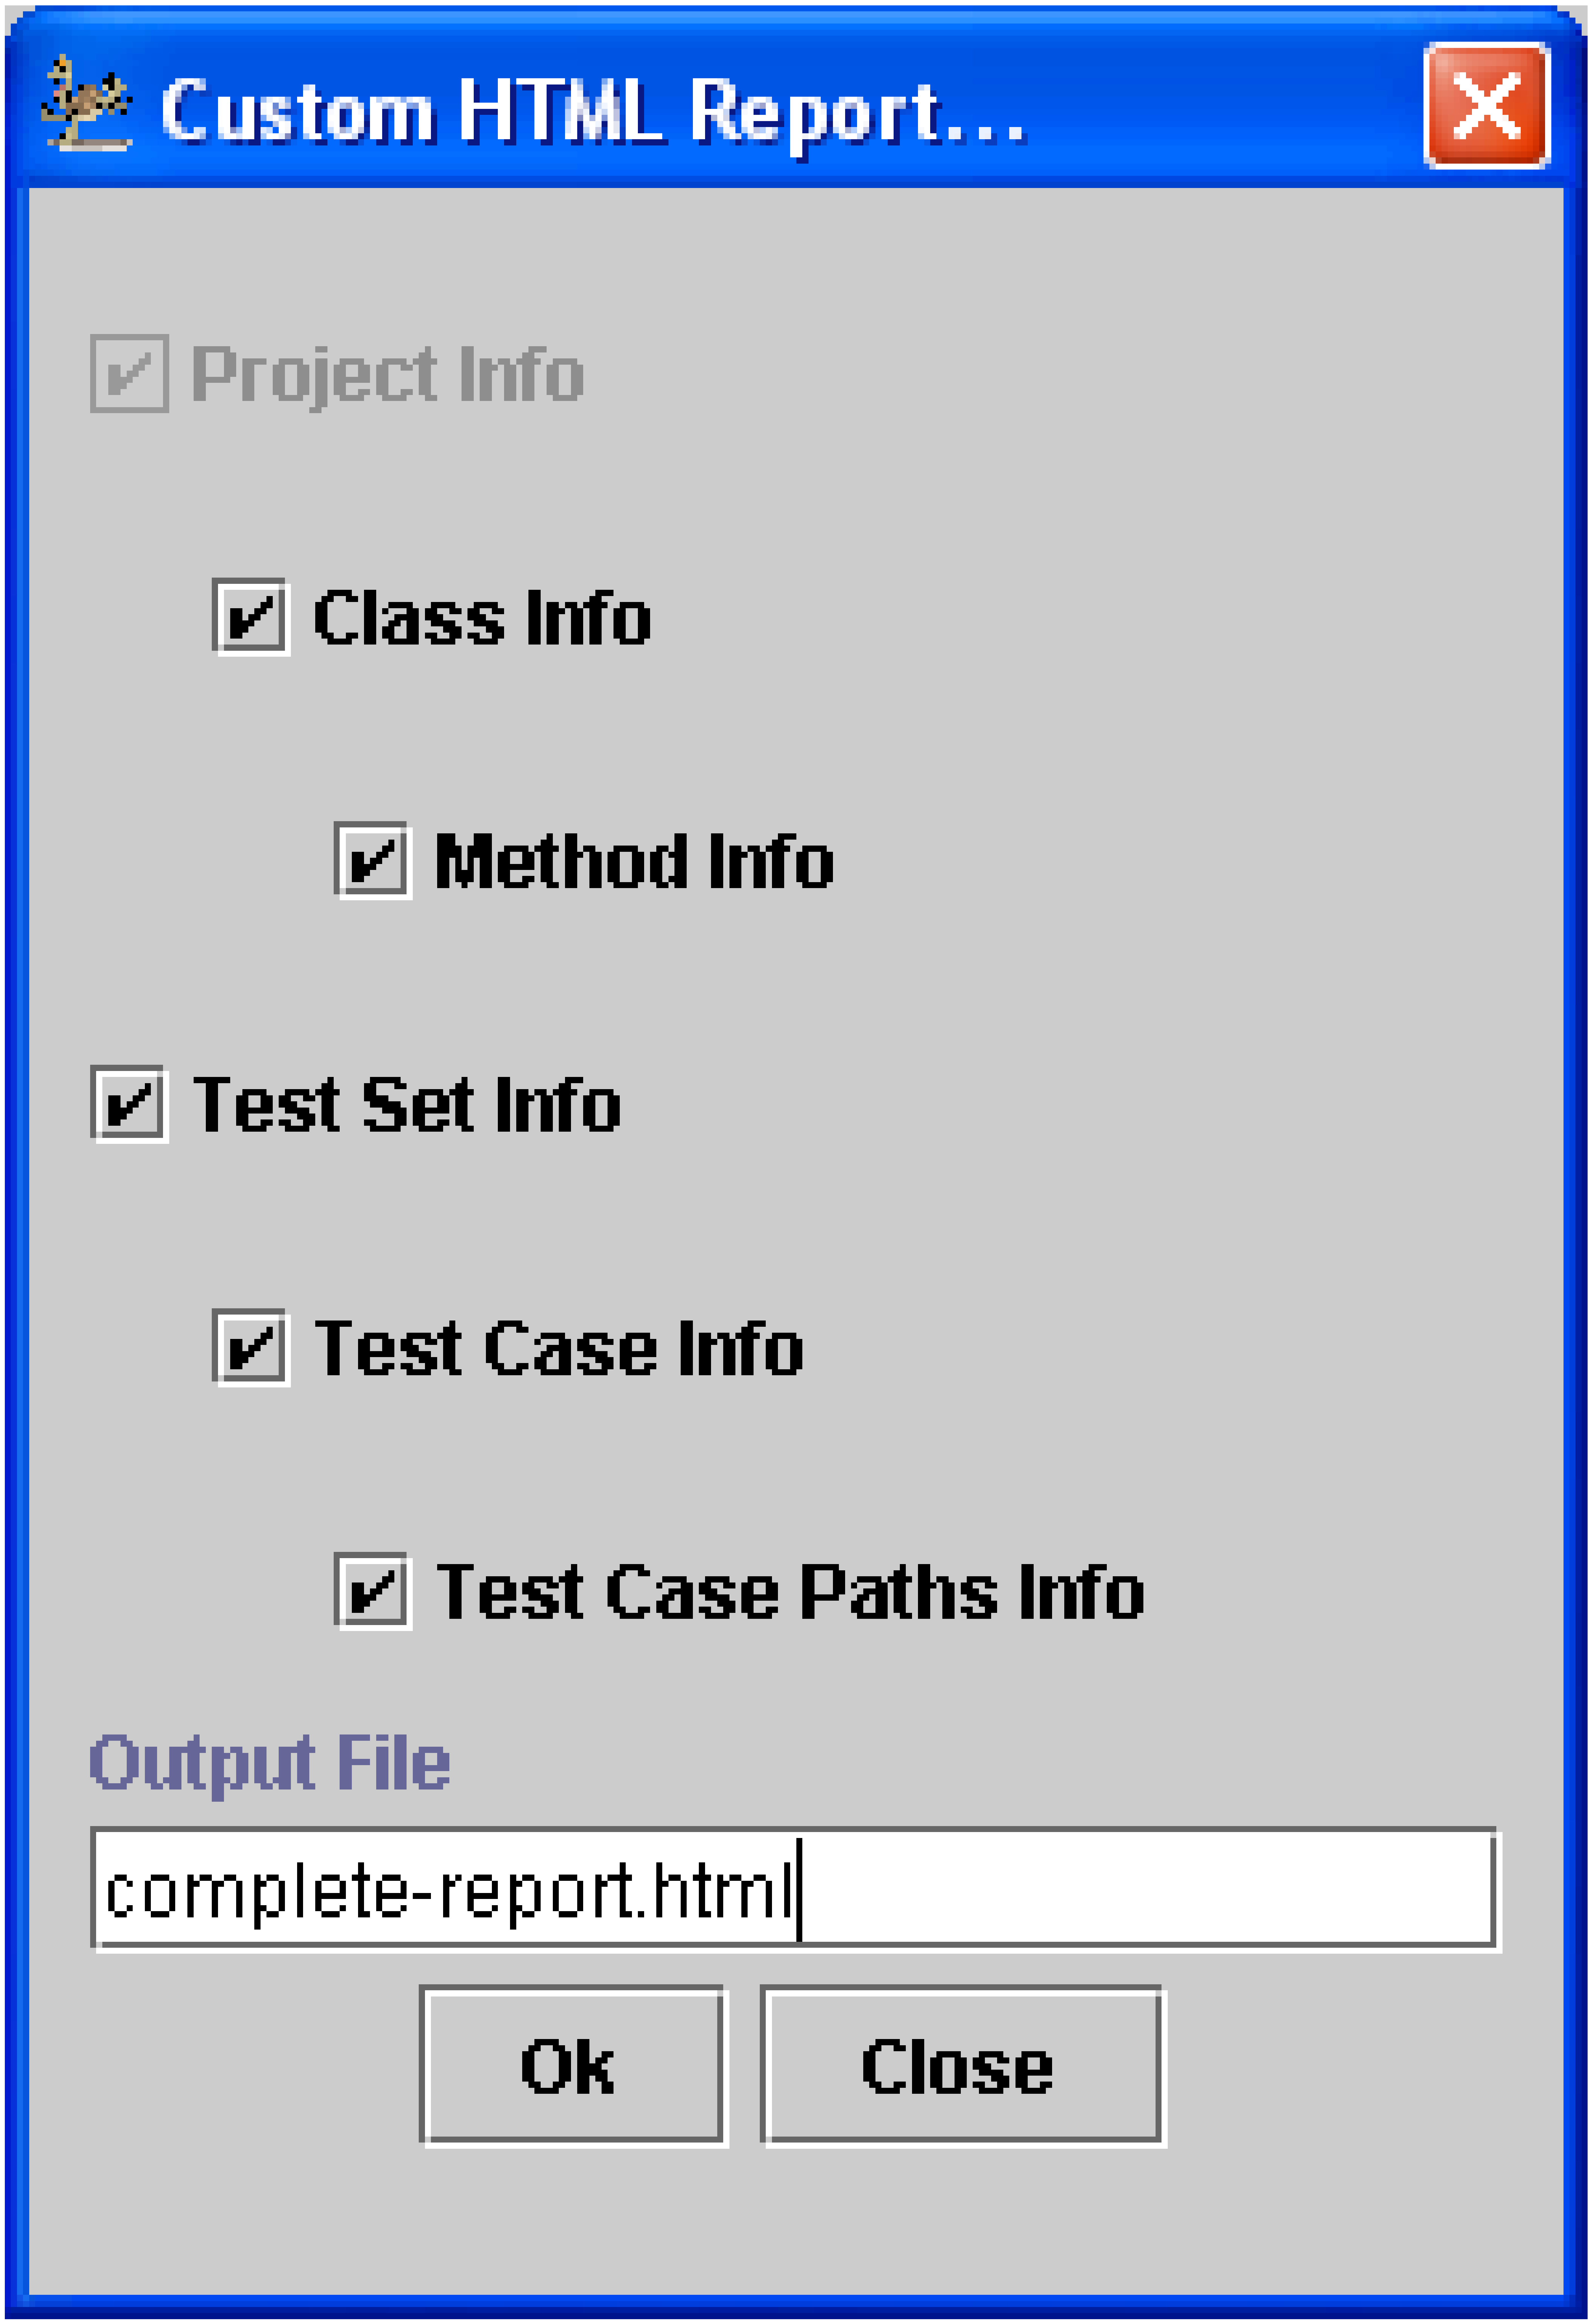
\includegraphics[width=0.25\textwidth]{fig/custom-html.eps}}\qquad
\subfigure[]{\label{fig:html-file2}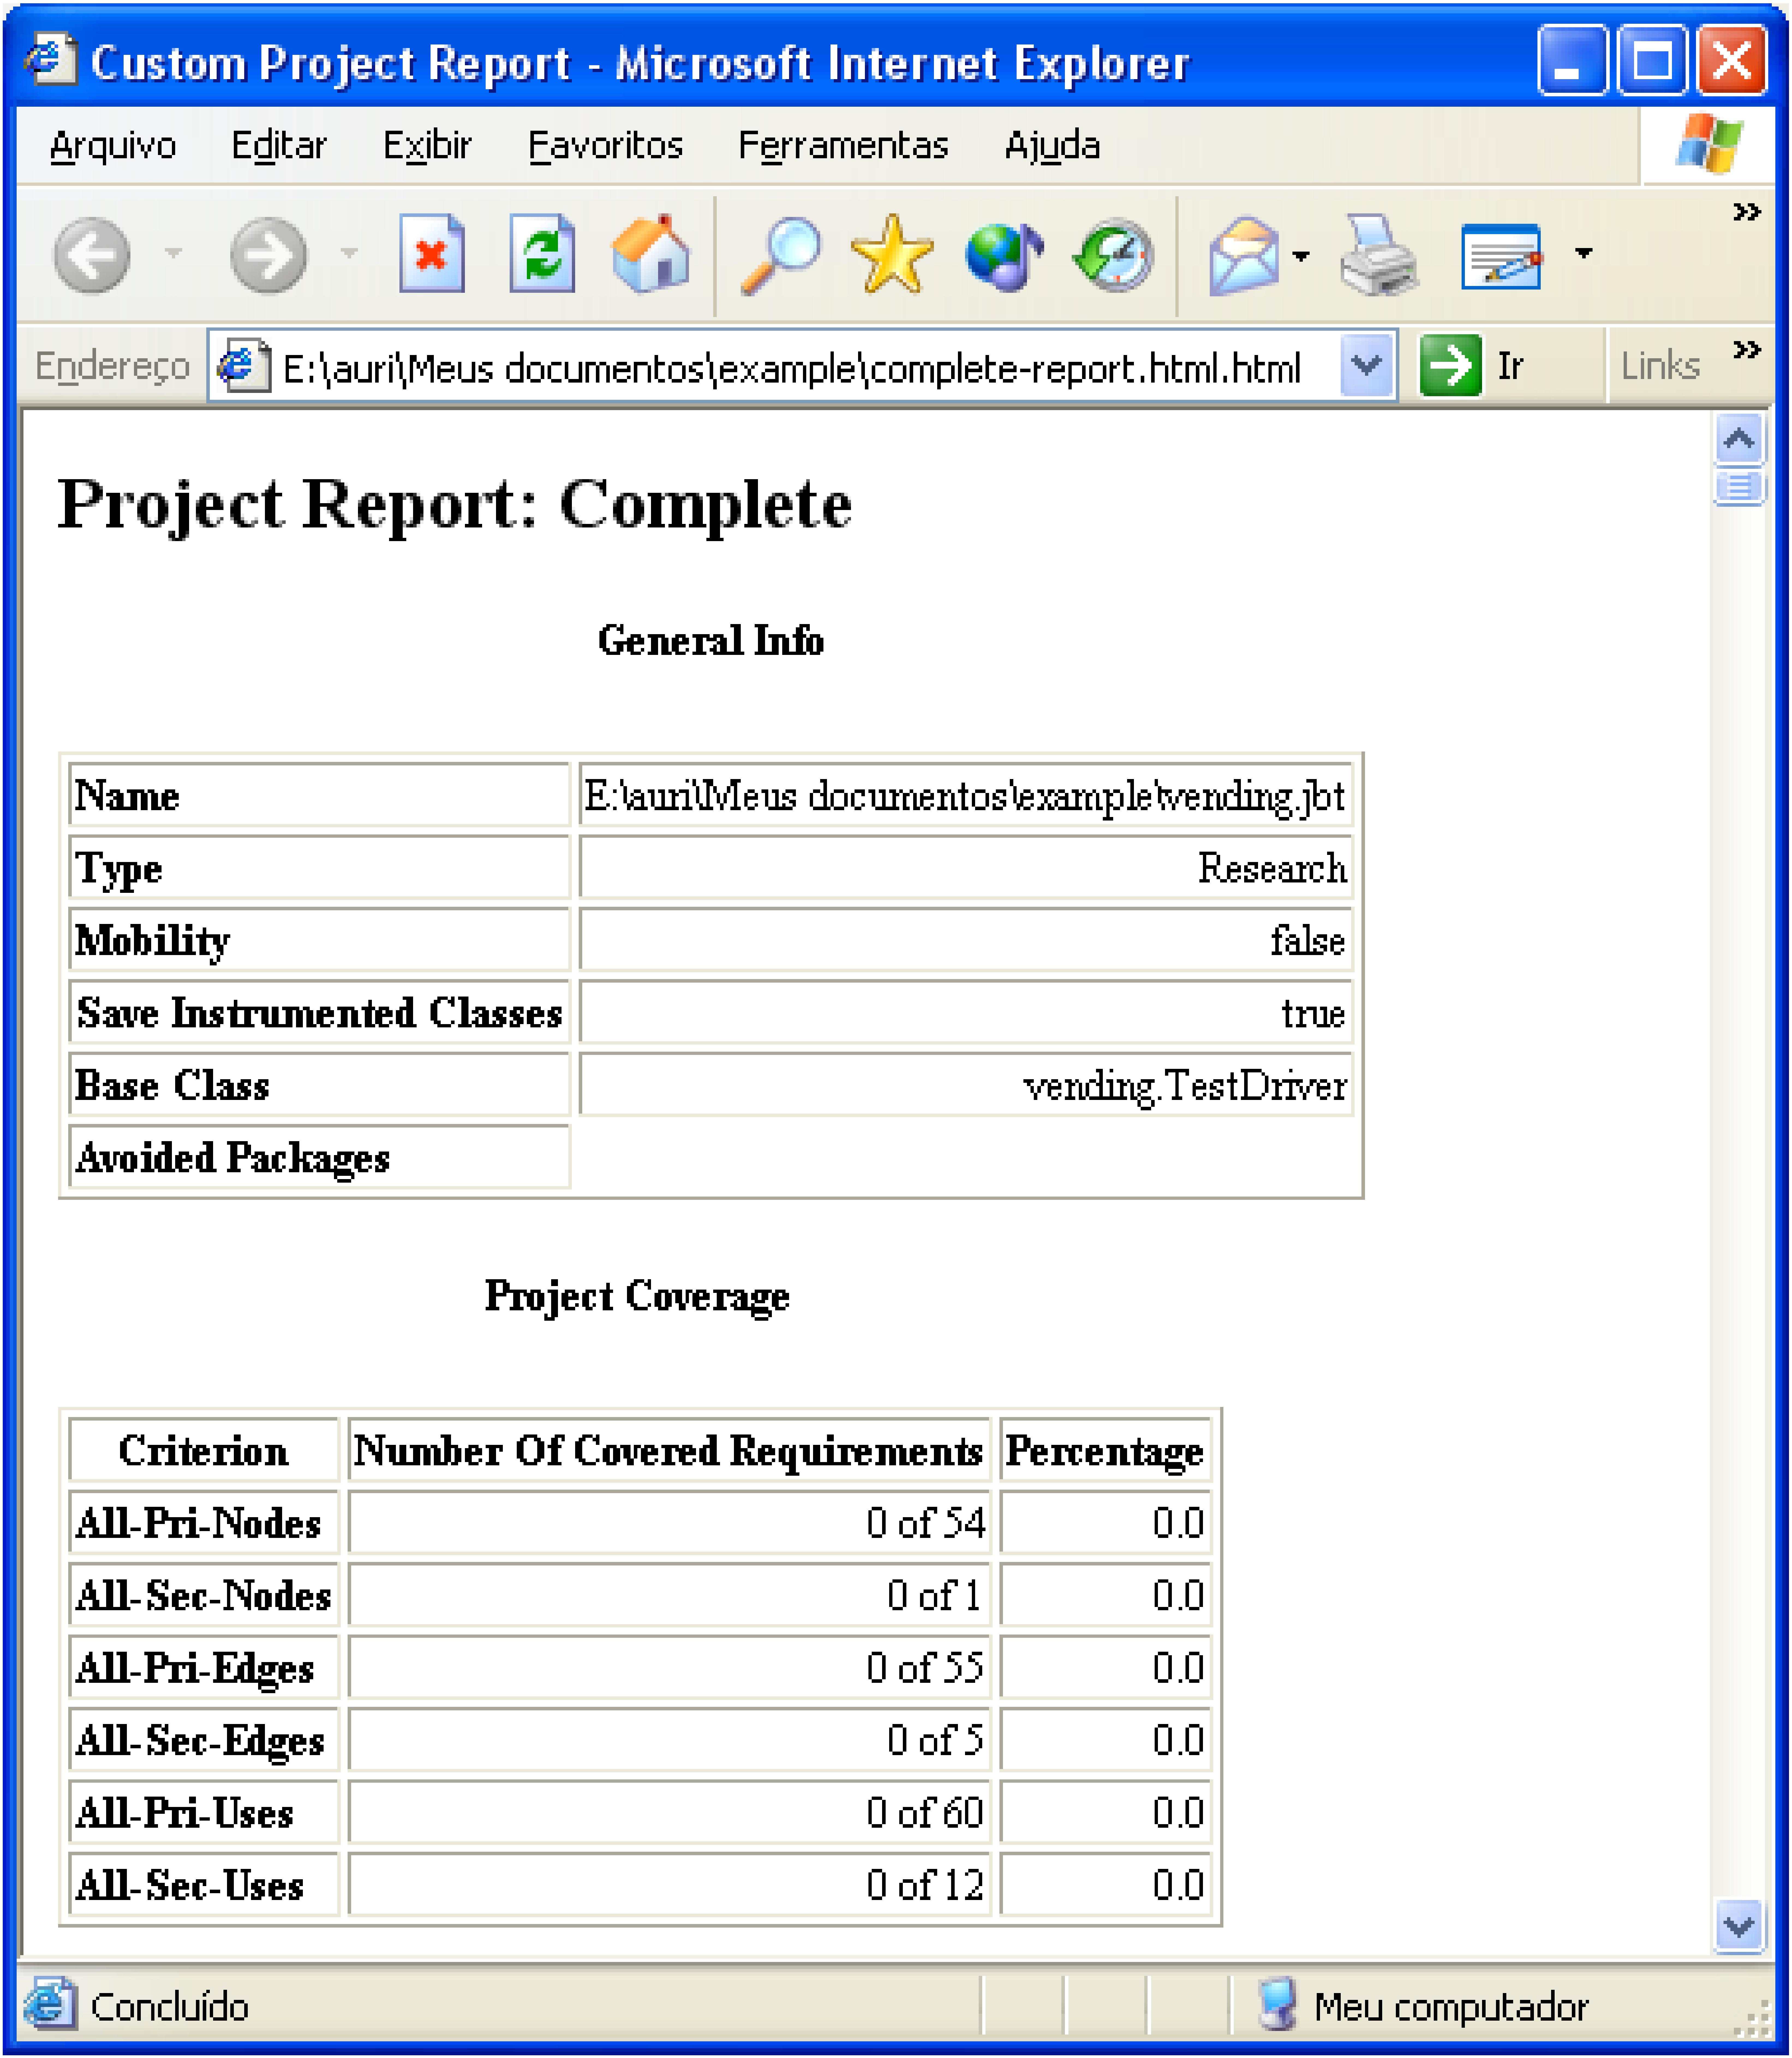
\includegraphics[width=0.45\textwidth]{fig/complete-html.eps}}
\caption{Example of custom HTML report generated by \toolname for
the entire project.}\label{fig:custom-html-report}
\end{center}
\end{figure}


\afterpage{\clearpage}
\newpage

\subsection{How to include a test case}\label{sec:testcase}

\toolname is designed to support test case set adequacy evaluation
and to provide guidance in test case selection. If there is a
previously developed test set, \eg a functional test set, such a
test set can be evaluated against the structural testing criteria
implemented by \toolname. This allows the tester to check, for
example, whether all instructions/statements are executed by a
particular test set. If they are not yet executed, additional test
cases can be developed to improve the quality of the previous test
set.

On the other hand, if there is no previous test set available, the
tester can use the hints provided by the tool to create test cases
aiming at to cover the different testing requirements generated by
\toolname based on its structural criteria. Once the test criteria
can be applied incrementally, the tester can start by developing
an adequate test set \wrt the \pk{All-Pri-Nodes} criterion, then,
if necessary, to develop additional test cases to evolve the
\pk{All-Pri-Nodes}-adequate test set to a
\pk{All-Pri-Edges}-adequate test set, and later, if necessary, to
develop additional test cases to evolve it to an
\pk{All-Pri-Uses}-adequate test set. All these criteria, prefixed
by \pk{All-Pri-}, are related with the normal program execution.
If desired, the tester can check the coverage of the
exception-handling mechanism, by using the \pk{All-Sec-Nodes},
\pk{All-Sec-Edges} and \pk{All-Sec-Uses} criteria. The idea is to
use these criteria incrementally to reduce their complexity and
also to allow the tester to deal with the cost and time
constraints.

\begin{sloppypar}
\toolname allows to include test cases in two different ways: 1)
using the \toolname's class loader; or 2) importing from a JUnit
test set. The first is done by a command line application
(\pk{probe.ProberLoader}, the \toolname's class loader). This
command line application extends the default Java class
loader~\cite{Lindholm99JVMS} such that, from a given testing
project, it identifies which classes should be instrumented before
to be loaded and executed. By detecting that a given class belongs
to the set of classes under testing, \toolname's class loader
inserts the probes to collect the execution trace and then loads
the instrumented class file to be executed. The trace information
\wrt the current execution is appended in a trace file with the
same name of the testing project but with the extension \trcext
instead of \prjext.
\end{sloppypar}

For example, the test case file \pk{input1}, presented in
Figure~\ref{fig:input1}, touches the testing requirement
(considering the \pk{All-Pri-Nodes} criterion) with the highest
weight illustrated in Figure~\ref{fig:dispenser-source} and also
reveals a fault contained in the \pk{Dispenser} component. Such a
test case will be used in the next section to show how to use
\toolname to ease the fault localization.

\begin{figure}[!ht]
\begin{cmd}
auri@AURIMRV ~/example
$ cat input1
insertCoin
vendItem 3
\end{cmd}
\vspace{-0.7cm} \caption{Example of test case
file.}\label{fig:input1}
\end{figure}

The command line in Figure~\ref{fig:driver-output}(a) shows the
output of the \pk{vending.TestDriver} when executed by the default
class loader. Figure~\ref{fig:driver-output}(b) shows the
resultant output when \pk{vending.TestDriver} is executed using
the \toolname's class loader. The execution of the command as
shown in Figure~\ref{fig:driver-output}(b) causes the
\pk{vending\trcext} to be generated/updated with the execution
path of test case file \pk{input1}.

\begin{figure}[!ht]
\begin{center}\cmdsize
\begin{tabular}{|c|c|}\hline
&\\
\begin{minipage}{2.7in}
\begin{verbatim}
auri@AURIMRV ~/example
$ java -cp "." vending.TestDriver input1
VendingMachine ON
Current value = 25
Enter 25 coins
Current value = -25
VendingMachine OFF







\end{verbatim}
\end{minipage}
&
\begin{minipage}{3.6in}
\begin{verbatim}
auri@AURIMRV ~/example
$ java -cp ".;..\Tools\jabuti;\
>..\Tools\jabuti\lib\BCEL.jar;\
>..\Tools\jabuti\lib\crimson.jar;\
> probe.ProberLoader -P vending.jbt \
> vending.TestDriver input1
Project Name: vending.jbt
Trace File Name: vending.trc
Processing File vending.jbt
VendingMachine ON
Current value = 25
Enter 25 coins
Current value = -25
VendingMachine OFF
\end{verbatim}
\end{minipage}\\
&\\\hline
\multicolumn{1}{c}{(a)} & \multicolumn{1}{c}{(b)}\\
\end{tabular}
\end{center}
\caption{\pk{vending.TestDriver} output: (a) default class loader, and (b)
\toolname class loader.}\label{fig:driver-output}
\end{figure}


Considering Figure~\ref{fig:driver-output}(b), observe that the
\pk{CLASSPATH} variable is set containing all the paths necessary
to run the \toolname's class loader and also the vending machine
example. The next parameter, \pk{probe.ProberLoader}, is the name
of the \toolname's class loader. It demands two parameters to
execute: the name of the project (\pk{-P vending.jbt}), and the
name of the base class to be executed (\pk{vending.TestDriver}).
In our example, since \pk{vending.TestDriver} requires one
parameter to be executed, this parameter is also provided
(\pk{input1}). During the execution of \pk{vending.TestDriver},
\pk{VendingMachine} and \pk{Dispenser} classes are required to be
loaded. From the project file (\pk{vending.jbt}) the \toolname's
class loader detects that these class files have to be
instrumented before to be executed. The instrumentation is
performed on-the-fly every time the \pk{probe.ProberLoader} is
invoked.

The resultant execution trace information, corresponding to the
execution of the test case \pk{input1}, is appended in the end of
the trace file \pk{vending\trcext}. Every time the size of the
trace file increase, the \pk{Update} button in the \toolname's
graphical interface becomes red, indicating that the coverage
information can be updated considering the new test case(s).
Figure~\ref{fig:update-button} illustrates this event.

\begin{figure}[!ht]
\begin{center}
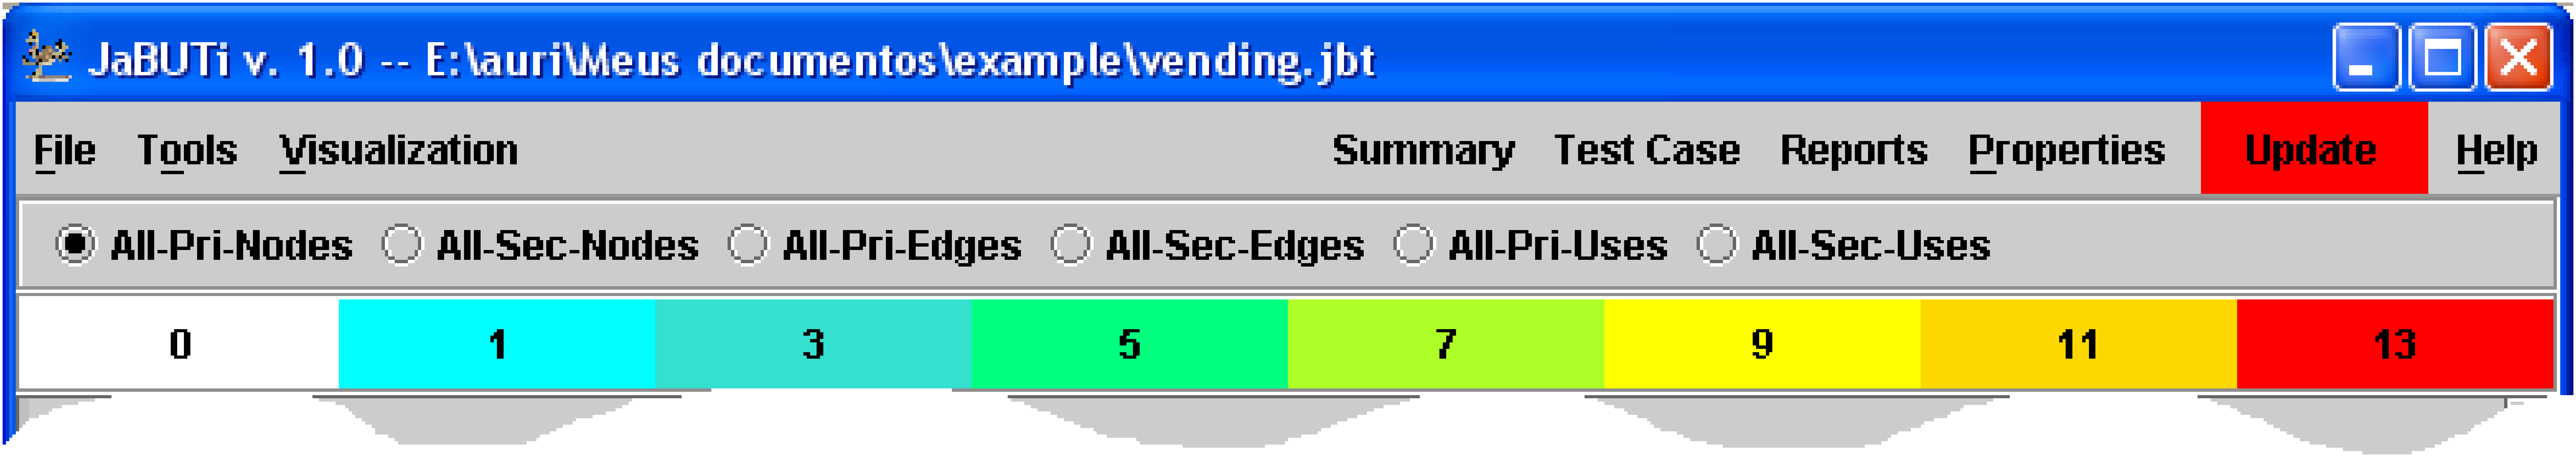
\includegraphics[width=0.70\textwidth]{fig/update-button.eps}
\caption{\label{fig:update-button} Update button with a different
background color: new test case(s) available.}
\end{center}
\end{figure}


By clicking on the \pk{Update} button, \toolname imports the new
test case(s), empties the trace file \pk{vending\trcext} and
updates the coverage information and the weights for each testing
criterion. For example, after the importation of test case
\pk{input1}, the weight of the Java source code \wrt the
All-Pri-Nodes criterion changed as illustrated in
Figure~\ref{fig:source-input1}.

\begin{figure}[!ht]
\begin{center}
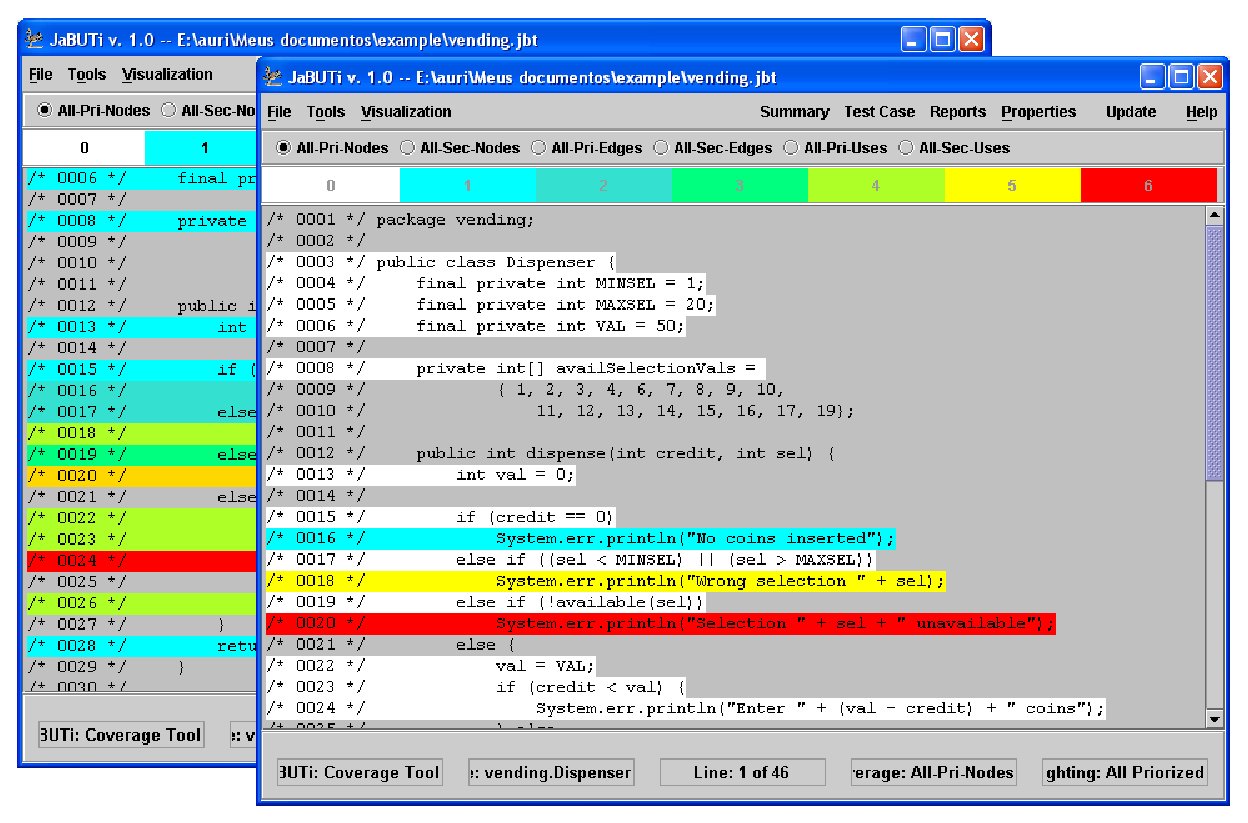
\includegraphics[height=0.40\textheight]{fig/dispenser-source-edited.eps}
\caption{\label{fig:source-input1} \pk{Dispenser.dispenser()}
method before and after the weight's updating \wrt
\pk{All-Pri-Nodes} criterion.}
\end{center}
\end{figure}


Comparing the updated source of Figure~\ref{fig:source-input1}
(front) with the one presented in Figure~\ref{fig:source-input1}
(back) it can be observed that the requirement with the highest
changed from source line 24 (now covered -- painted in white) to
source line 20. Considering the entire project,
Figure~\ref{fig:summary-method-tc1} shows the updated coverage for
each method in the \pk{Dispenser} and \pk{VendingMachine} classes
\wrt the \pk{All-Pri-Nodes} criterion. Observe that \pk{input1}
covered 13 primary nodes (50\%) of \pk{Dispenser.dispense} method
and 36 of 56 primary nodes (64\%) considering the entire project.
By accessing the \pk{Test Case $\rightarrow$ Report by Test Case}
menu option, the tester can visualize the coverage of the entire
project by test case, as illustrated in
Figure~\ref{fig:report_tc1}.

\begin{figure}[!ht]
\begin{center}
\subfigure[Report by test
case]{\label{fig:report_tc1}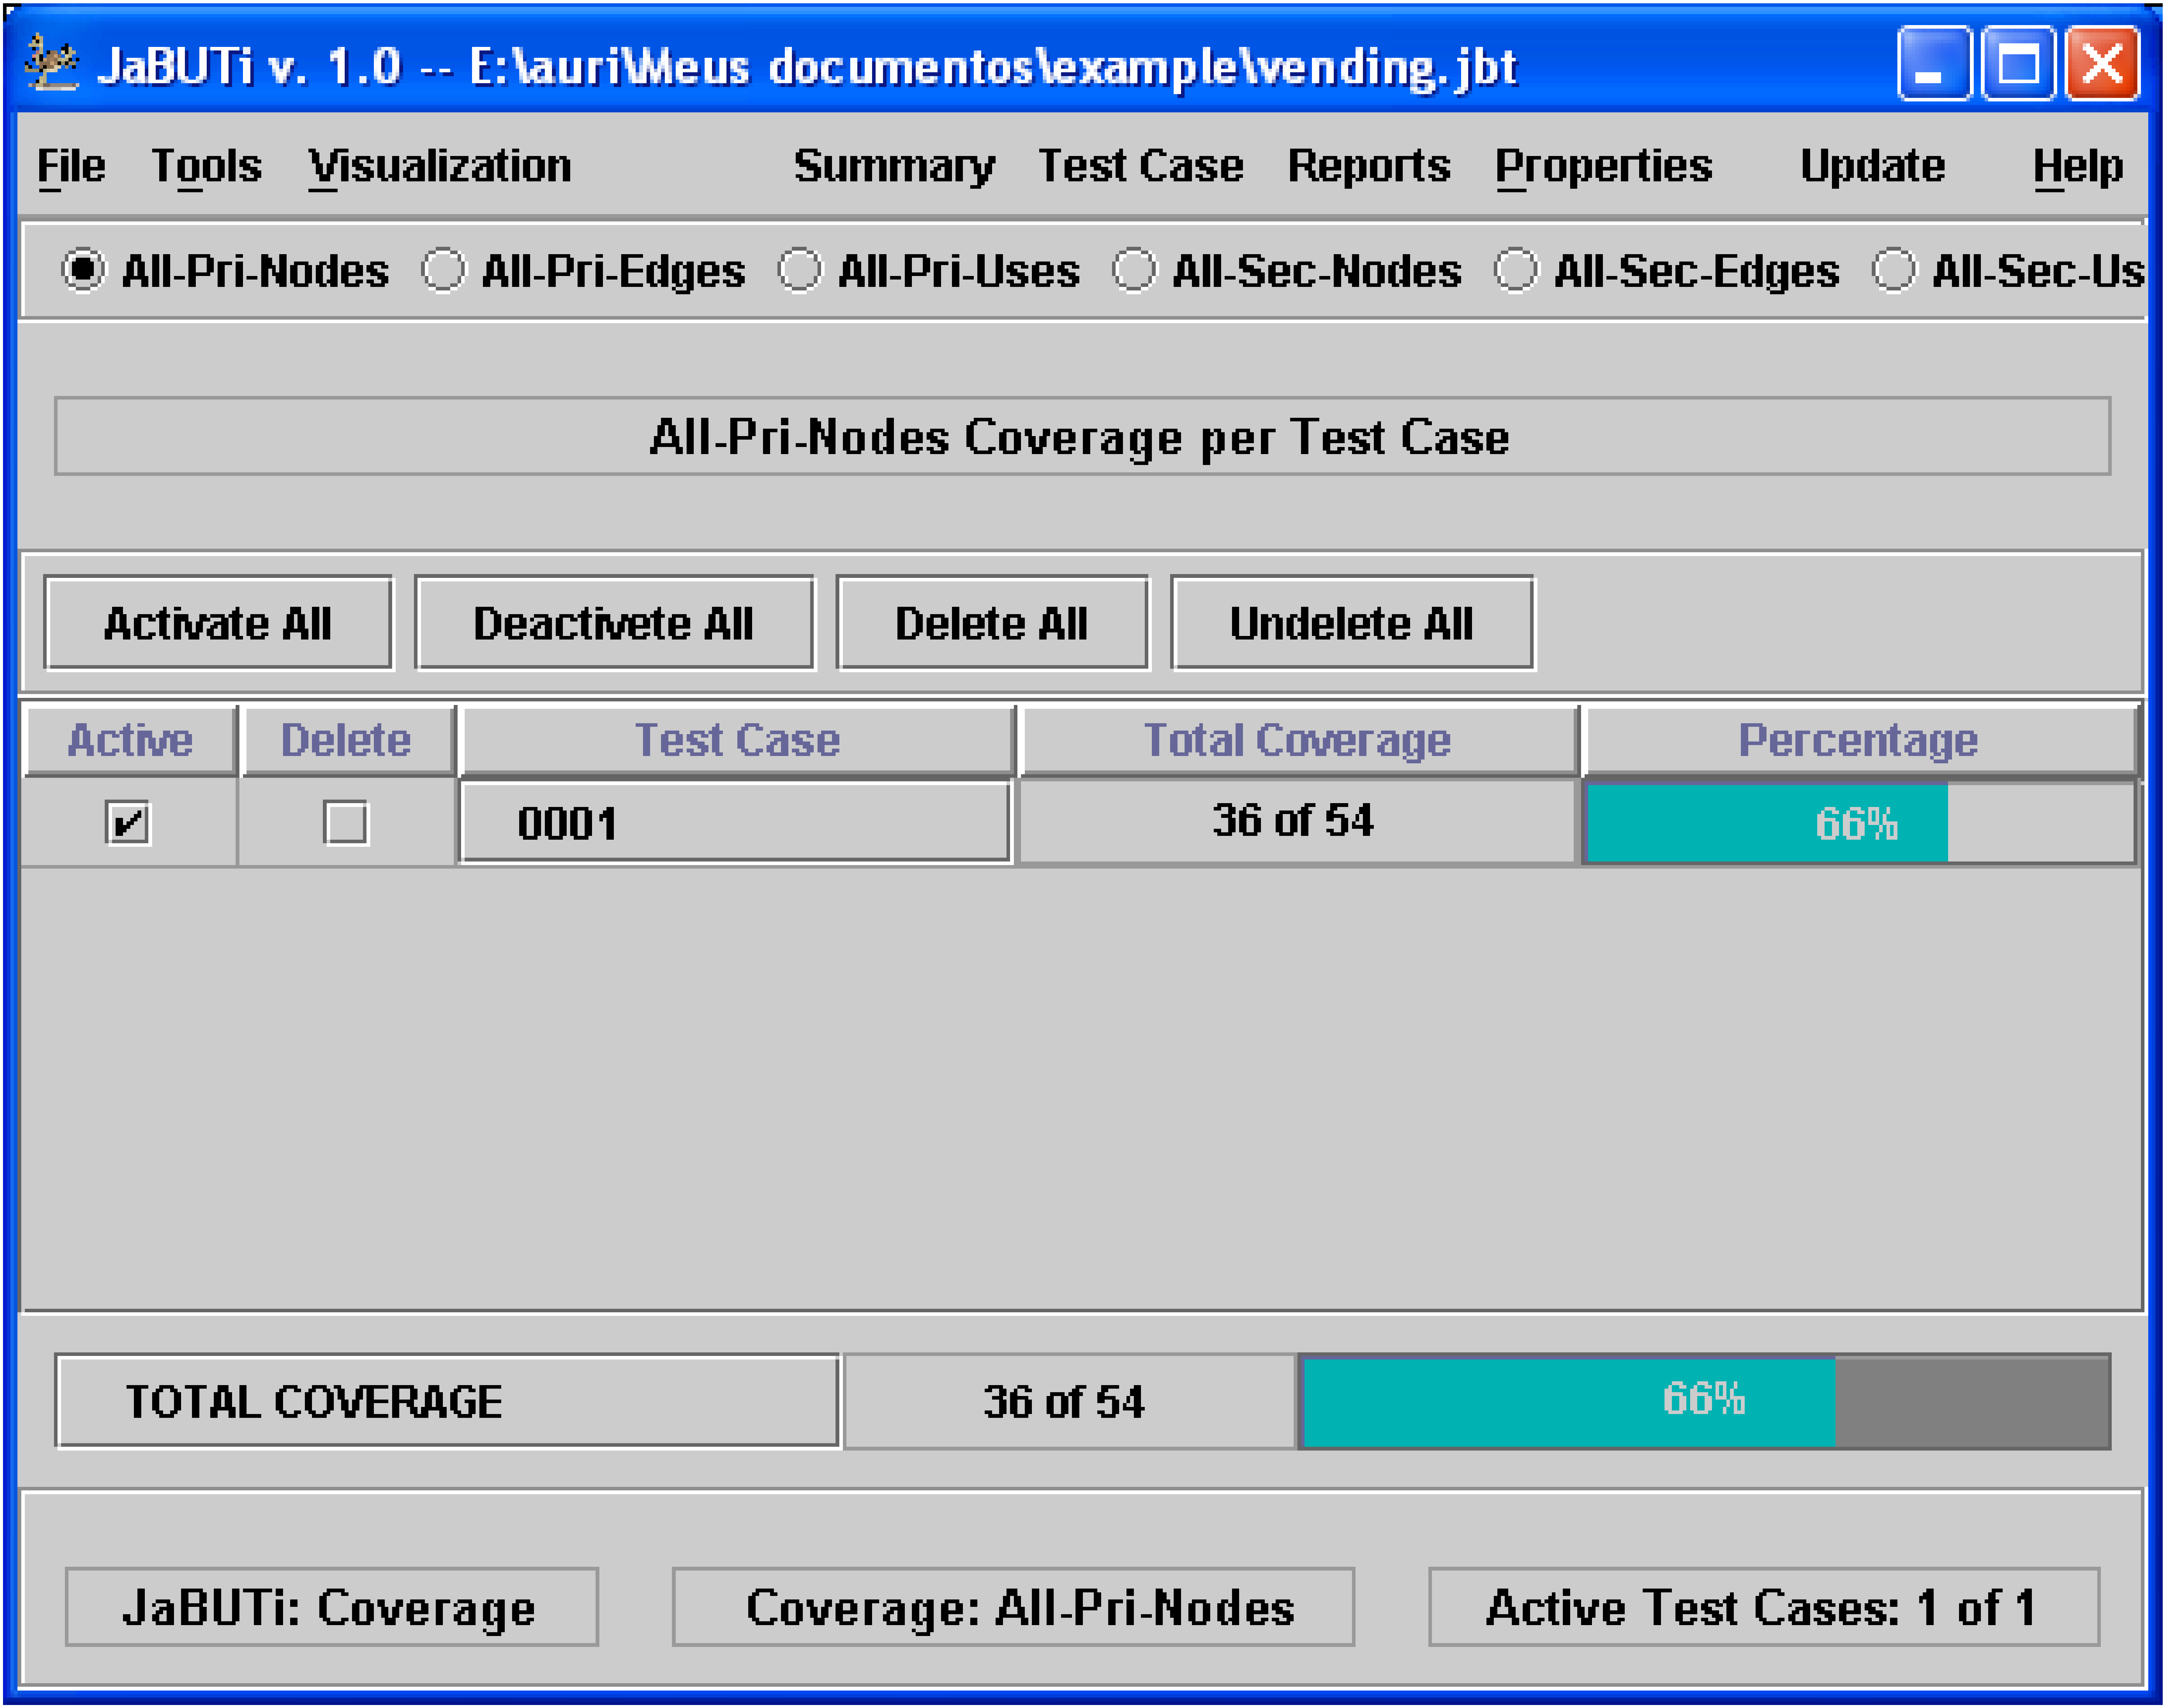
\includegraphics[width=0.40\textwidth]{fig/report-by-test-case-tc1.eps}}\qquad
\subfigure[Summary by
Method]{\label{fig:summary-method-tc1}\includegraphics[width=0.50\textwidth]{fig/summary-by-method-tc1.eps}}
\caption{Updated coverage after test case
\pk{input1}.}\label{fig:tc1}
\end{center}
\end{figure}


If desired, the tester can develop additional test cases to
improve the coverage \wrt \pk{All-Pri-Nodes} criterion. For
example, besides \pk{input1}, Table~\ref{tab:adequate} shows four
additional test cases developed to improve the coverage of such a
criterion.

\begin{table}[!ht]
\caption{Adequate test set to the \pk{Dispenser}
component.}\label{tab:adequate}
\begin{center}
\begin{tabular}{|l|l|l|}\hline
\textbf{Name} & \textbf{Content} & \textbf{Correct output}\\
\hline
input1  &   insertCoin      & no  \\
        &   vendItem 3      &     \\ \hline
input2  &   insertCoin      & yes \\
        &   vendItem 18     &     \\ \hline
input3  &   insertCoin      & yes \\
        &   insertCoin      &     \\
        &   vendItem 25     &     \\ \hline
input4  &   vendItem 3      & yes \\ \hline
input5  &   insertCoin      & yes \\
        &   insertCoin      &     \\
        &   vendItem 3      &     \\ \hline
\end{tabular}
\end{center}
\end{table}

\begin{sloppypar}
\toolname also allows to visualize the coverage of a given test
case by each execution path (\pk{Test Case $\rightarrow$ Report by
Test Case Path}), i.e., during the execution of a single test
case, several methods can be executed, and each one can be
executed several times. Each method execution is considered as a
different execution path. Therefore, a test case is composed by
zero or more test paths, one for each individual method execution.
Figure~\ref{fig:report-by-test-path} shows this kind of report.
For instance, test case \pk{0001} is composed by six paths
numbered from \pk{0001-0} to \pk{0001-5}. Besides the coverage by
path, the report also shows additional information about each
path, collected during the execution.
\end{sloppypar}

\begin{figure}[!ht]
\begin{center}
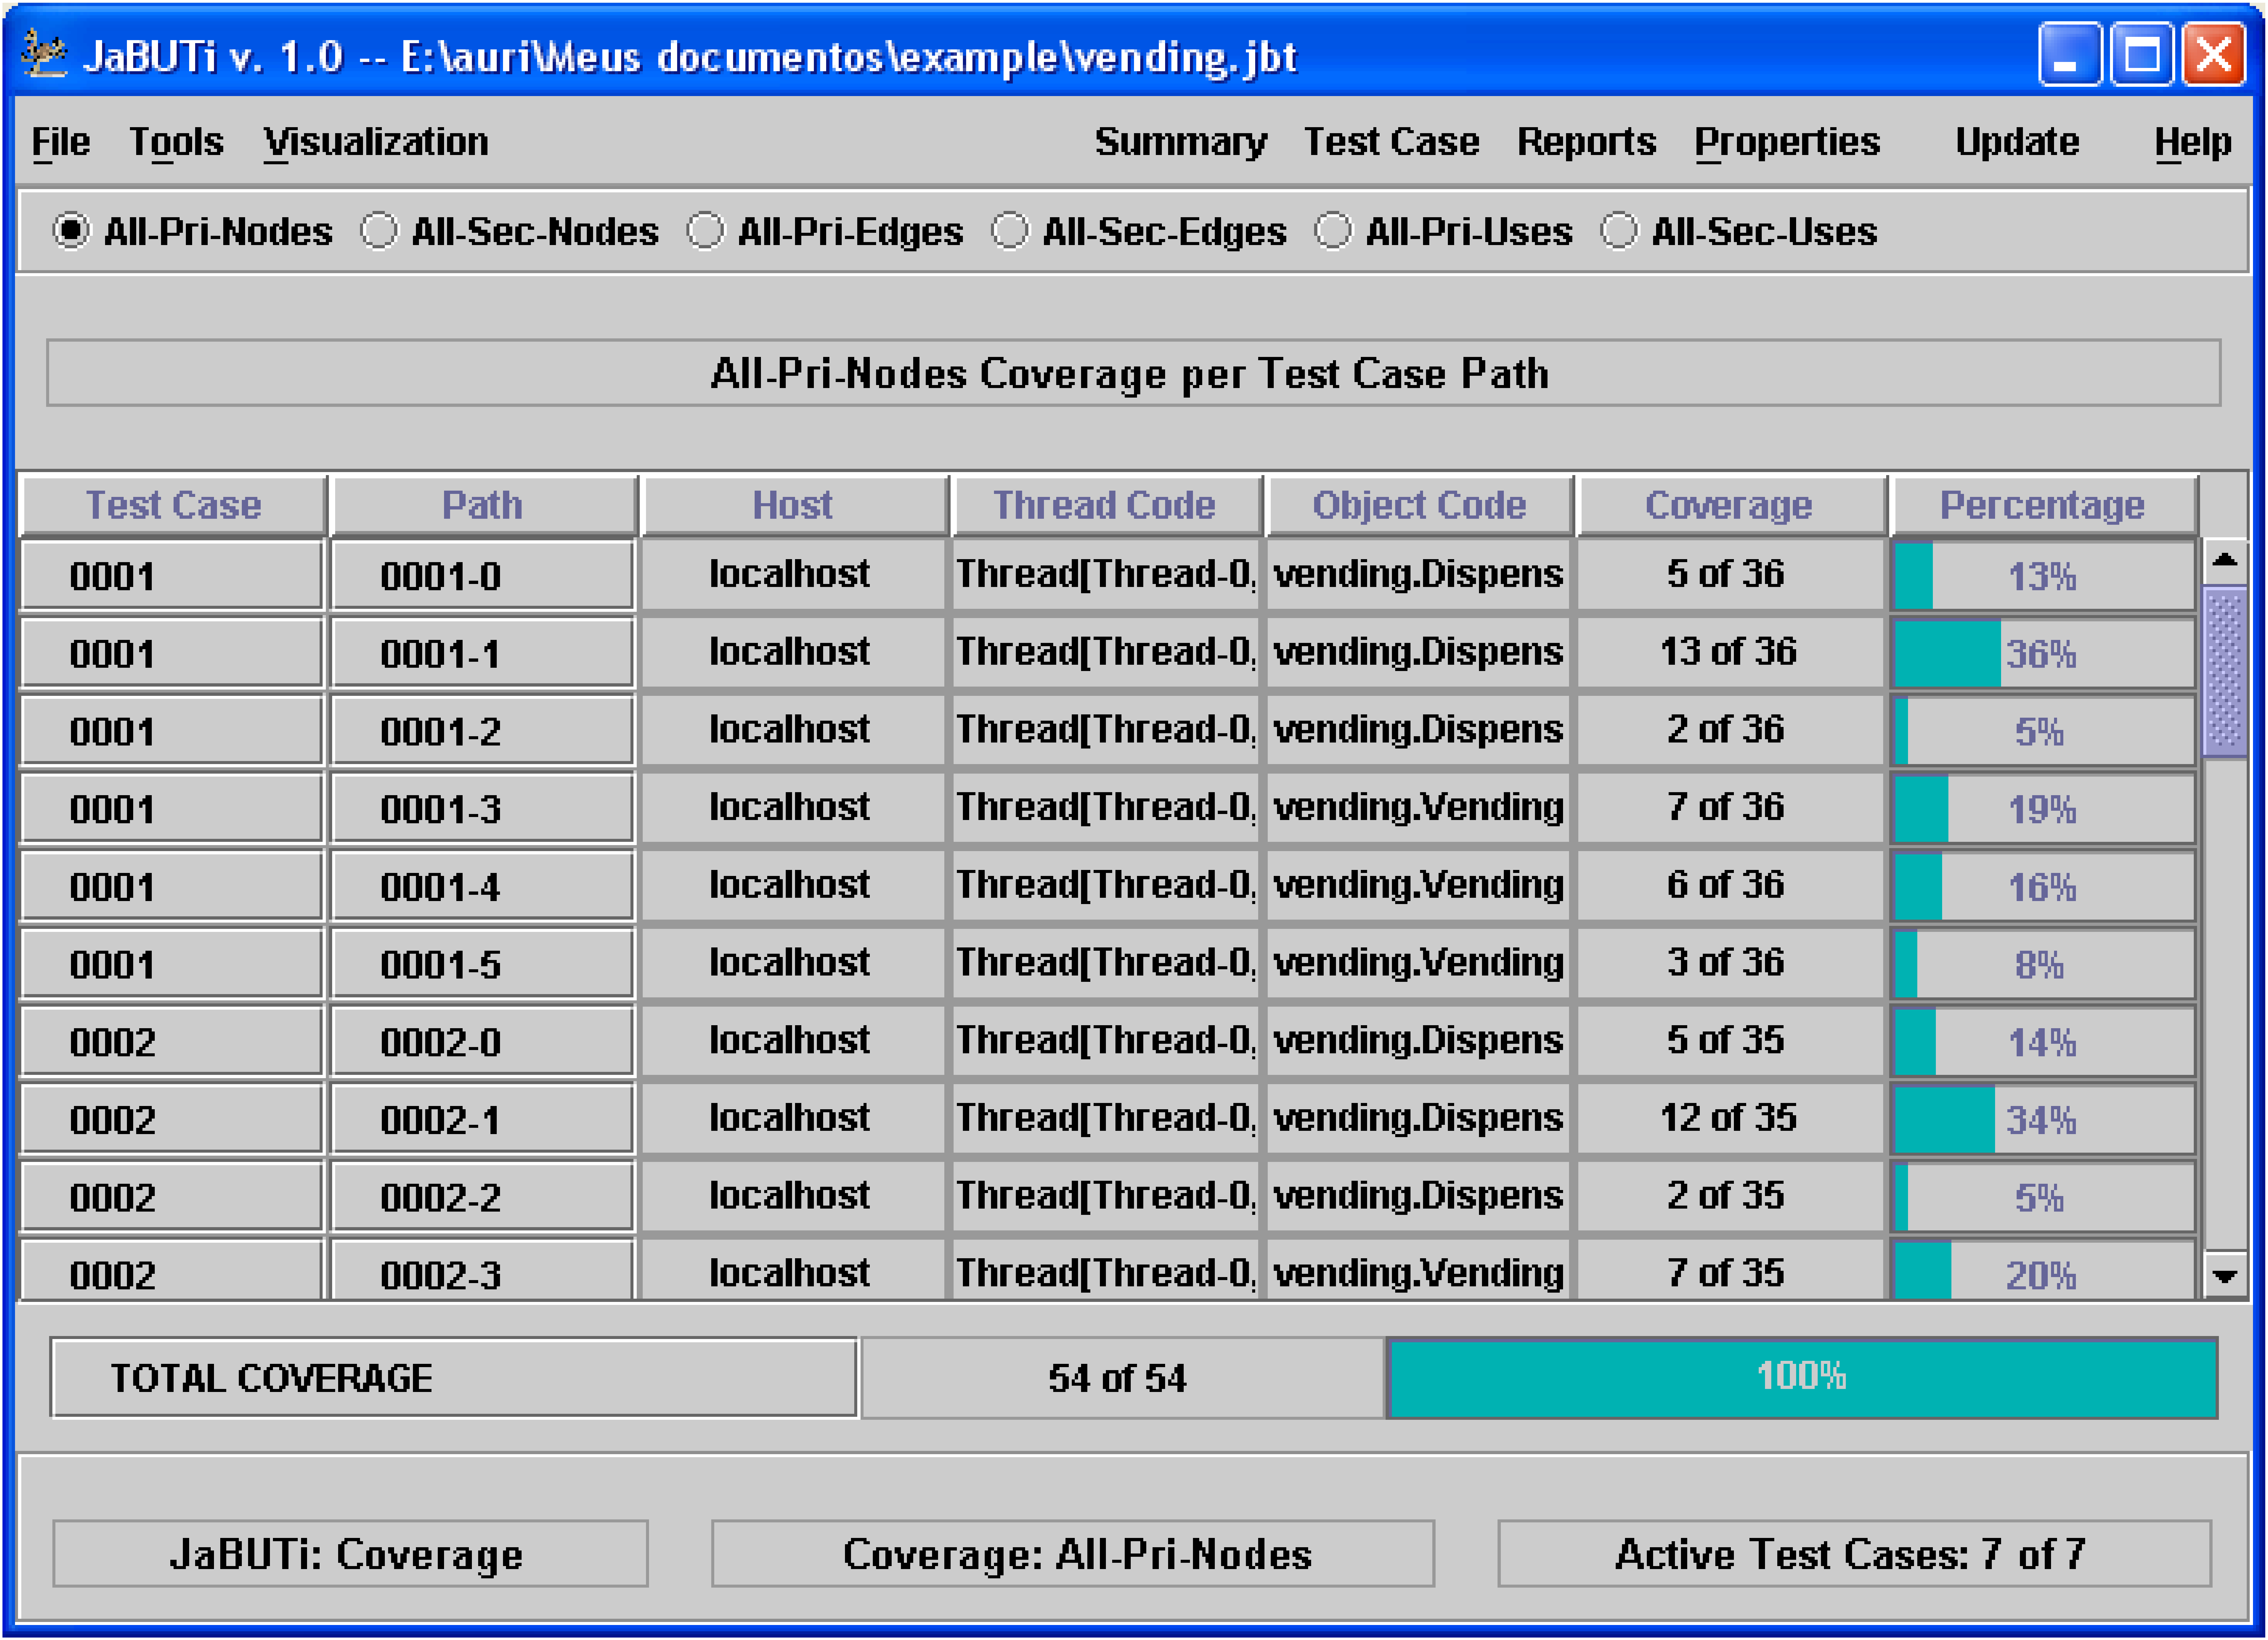
\includegraphics[width=0.70\textwidth]{fig/report-by-test-path.eps}
\caption{\label{fig:report-by-test-path} Testing report by
execution path \wrt the \pk{All-Pri-Nodes} criterion.}
\end{center}
\end{figure}


\afterpage{\clearpage}
\newpage

\subsection{How to import test cases from JUnit framework}

Observe that after five test cases, the coverage of almost all
methods, \wrt the \pk{All-Pri-Nodes} criterion, is 100\%. The only
two methods uncovered are \pk{Dispenser.setValidSelection()} and
\pk{VendingMachine.returnCoin()}. To obtain a adequate test set
\wrt the \pk{All-Pri-Nodes}, additional test cases are required.
Figure~\ref{fig:junit} shows one additional test case, specified
according to the JUnit framework, to cover 100\% of required
elements of the \pk{All-Pri-Nodes} for the \pk{Dispenser} class.
More information about how to develop test set using the JUnit
framework can be found
elsewhere~\cite{JUnit02UDCA,Rainsberger03JSGU}.

\begin{figure}[!ht]
\begin{center}
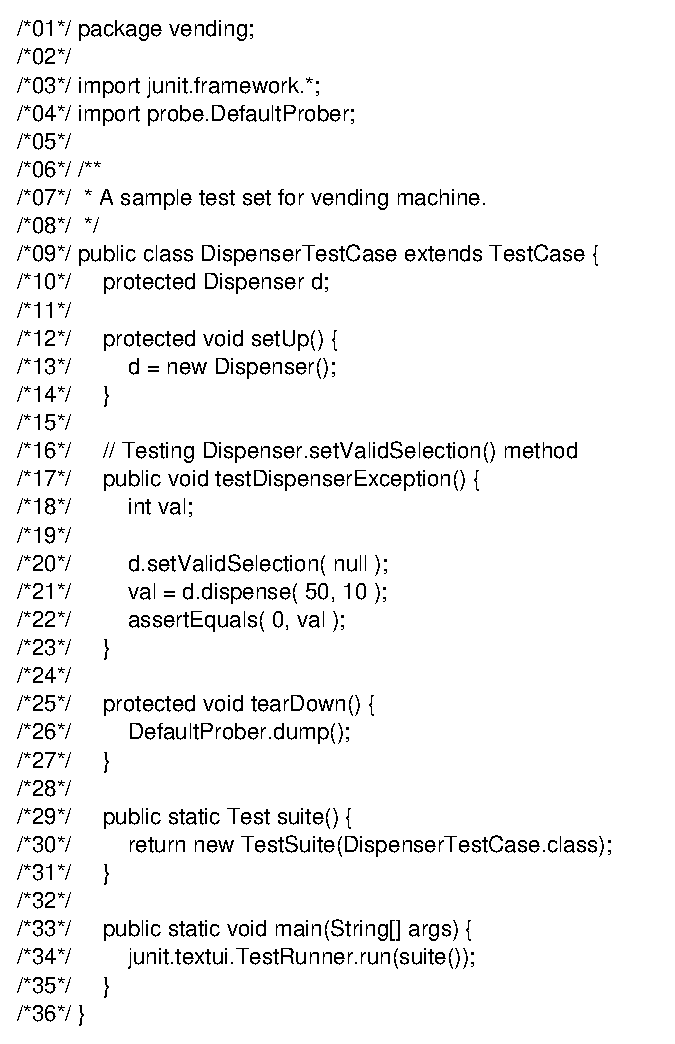
\includegraphics[width=0.4\textwidth]{fig/junit-test-case.eps}
\caption{\label{fig:junit}Example of a test set using the JUnit
framework.}
\end{center}
\end{figure}


As can be observed in Figure~\ref{fig:junit}, line 26, \toolname
requires that a static method (\pk{DefaultProber.dump()}) to be
called at the end of each test case\footnote{JUnit has two special
methods \pk{TestCase.setUp()} and \pk{TestCase.tearDown()}. The
former is executed before any test case execution and the later
after a test case execution. Therefore, since we want to execute
the method \pk{DefaultProber.dump()} after the execution of each
test case, a call to such a method is placed inside the method
\pk{TestCase.tearDown()}.}. Such a method is responsible to write
the execution trace in the trace file. Observe that to call such a
static method it is also necessary to include the import statement
as shown in line 04. Once compiled, such a JUnit test case can be
imported by \toolname from the \pk{Test Case $\rightarrow$ Import
from JUnit} menu option. Figure~\ref{fig:importing-junit} shows
the sequence of screens to import a JUnit's test case.

\begin{enumerate}
    \item Click on the \pk{Browser} button
    (Figure~\ref{fig:junit1});

    \item Select the directory where the JUnit test case class file is located
    (Figure~\ref{fig:junit2});

    \item Select the JUnit test case class file (\pk{DispenserTestCase.class}
    -- Figure~\ref{fig:junit3});

    \item Select the test cases to be imported and click on the
    \pk{Import Selected} button (Figure~\ref{fig:junit4}).
\end{enumerate}

\begin{figure}[!ht]
\begin{center}
\subfigure[]{\label{fig:junit1}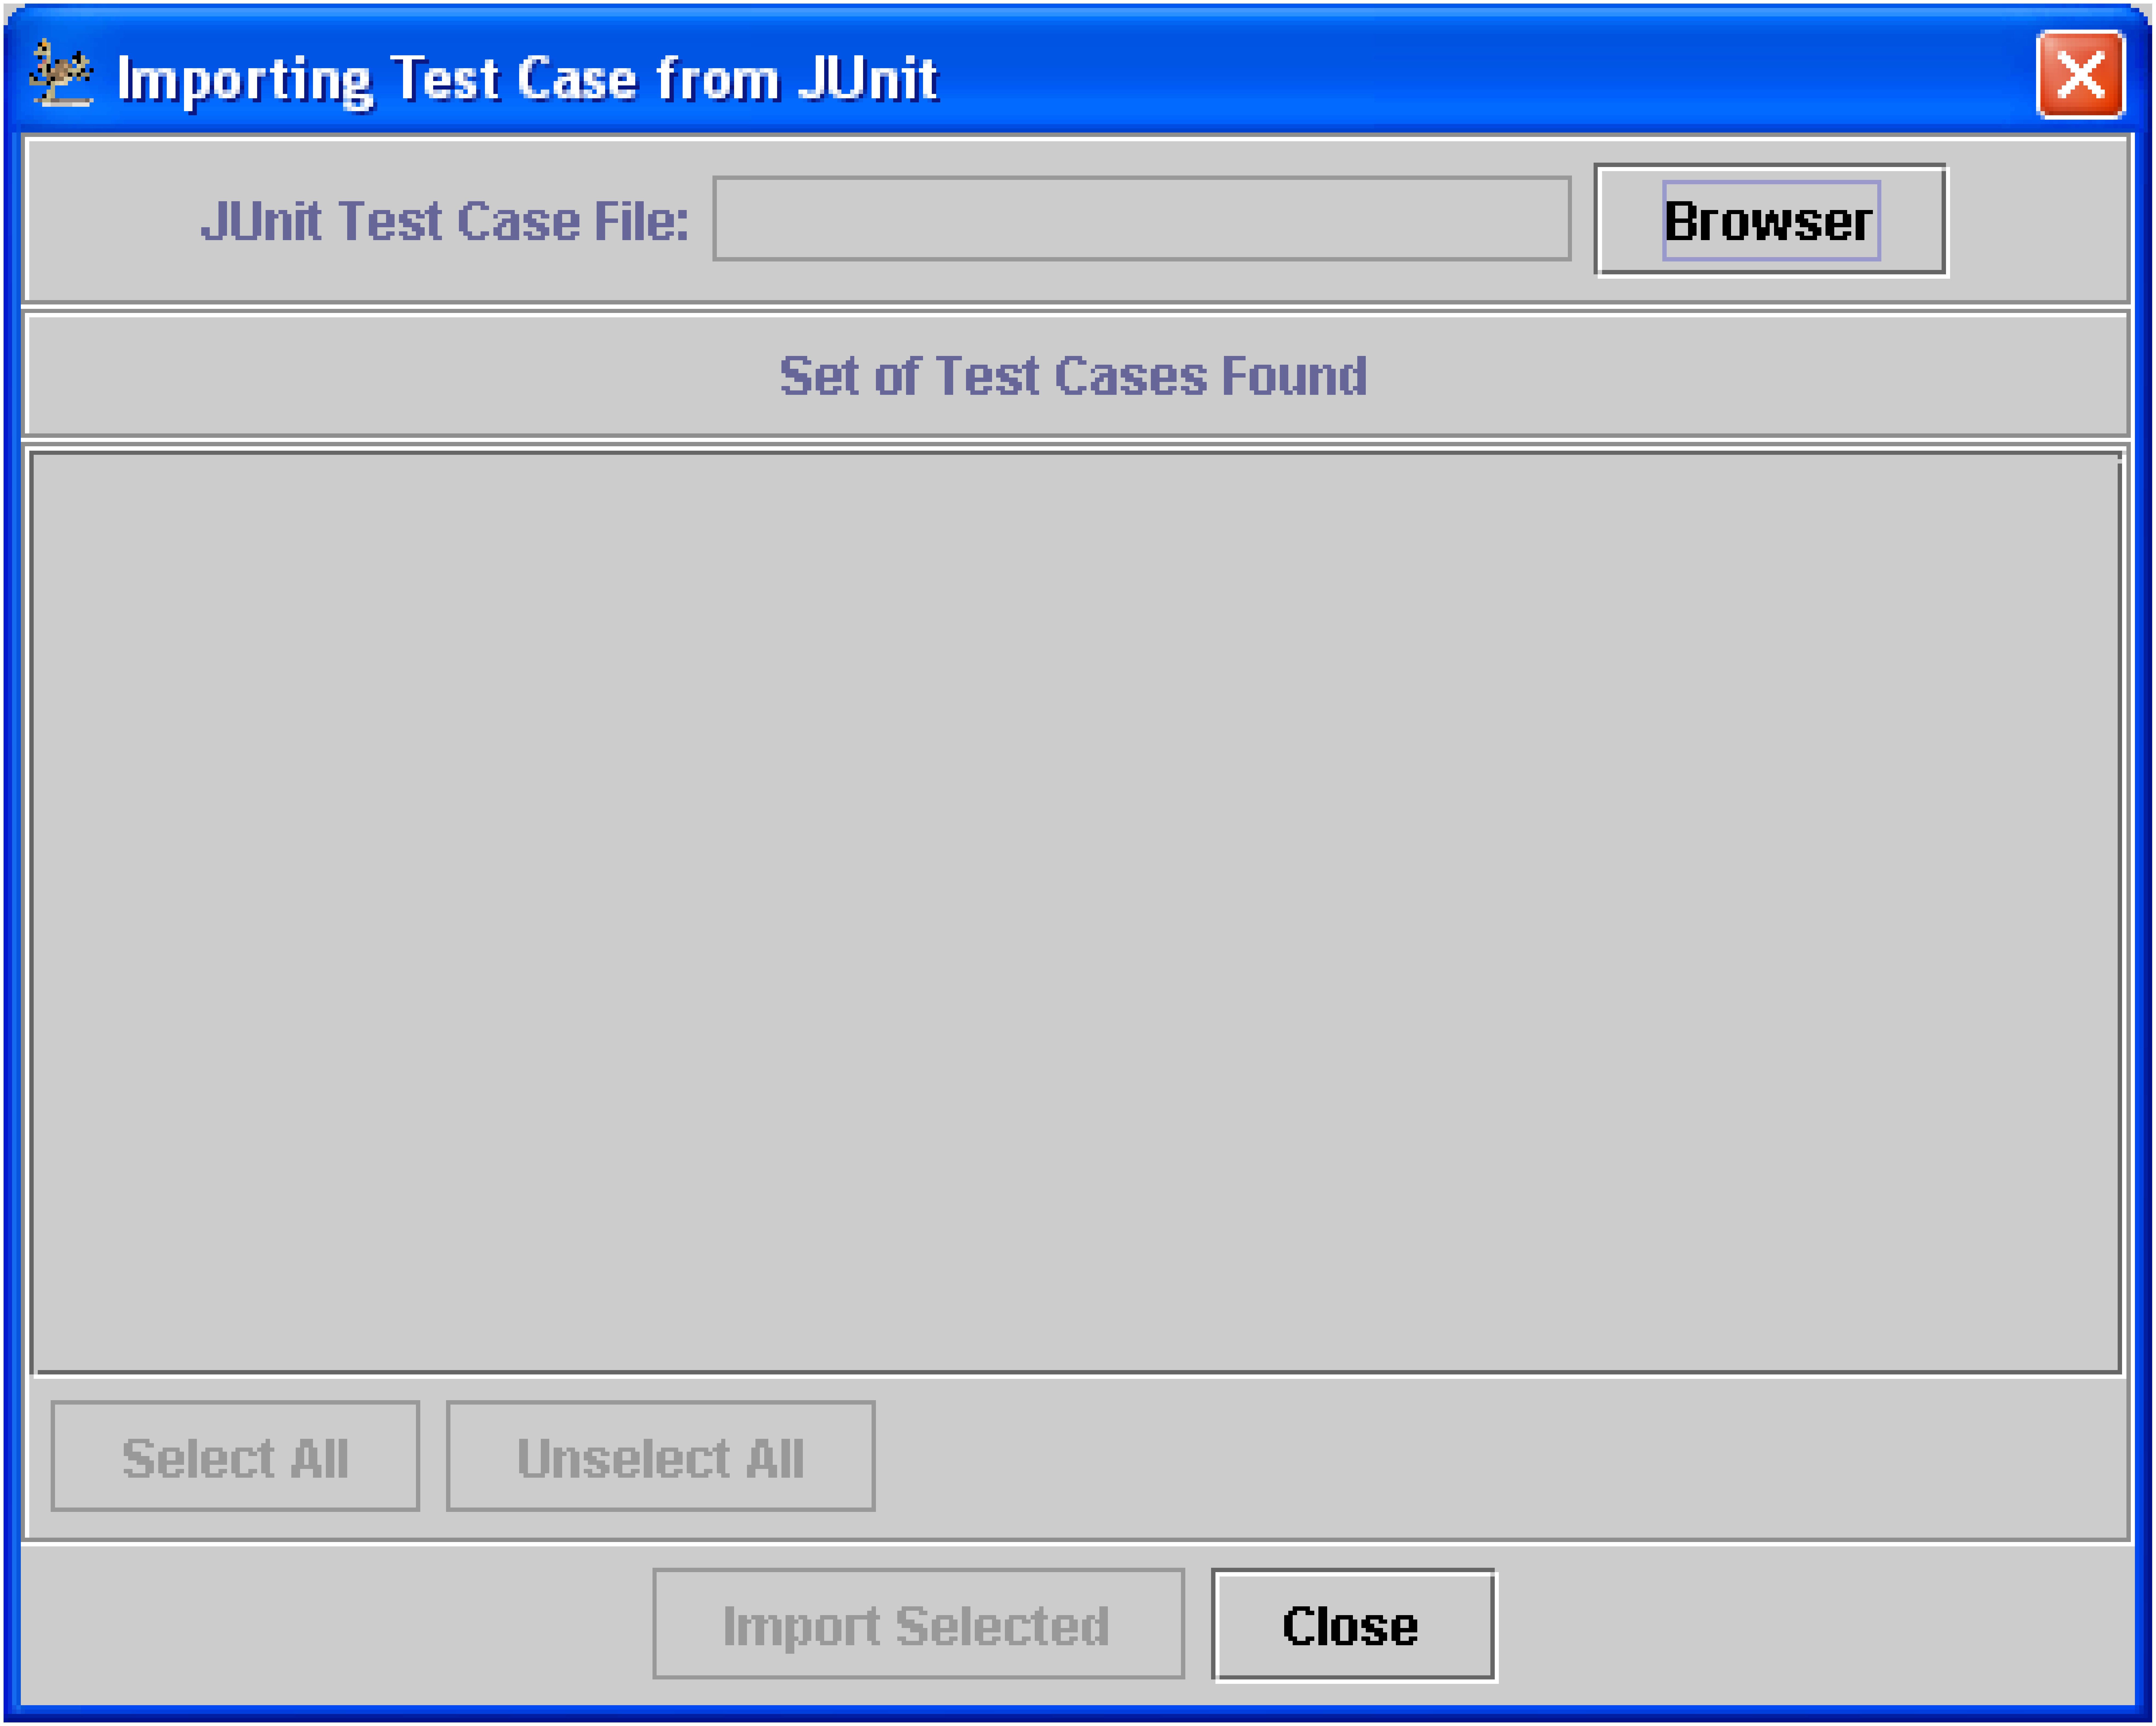
\includegraphics[width=0.45\textwidth]{fig/importing-junit-1.eps}}\quad
\subfigure[]{\label{fig:junit2}
\includegraphics[width=0.45\textwidth]{fig/importing-browser-1.eps}}

\subfigure[]{\label{fig:junit3}\includegraphics[width=0.45\textwidth]{fig/importing-browser-2.eps}}\quad
\subfigure[]{\label{fig:junit4}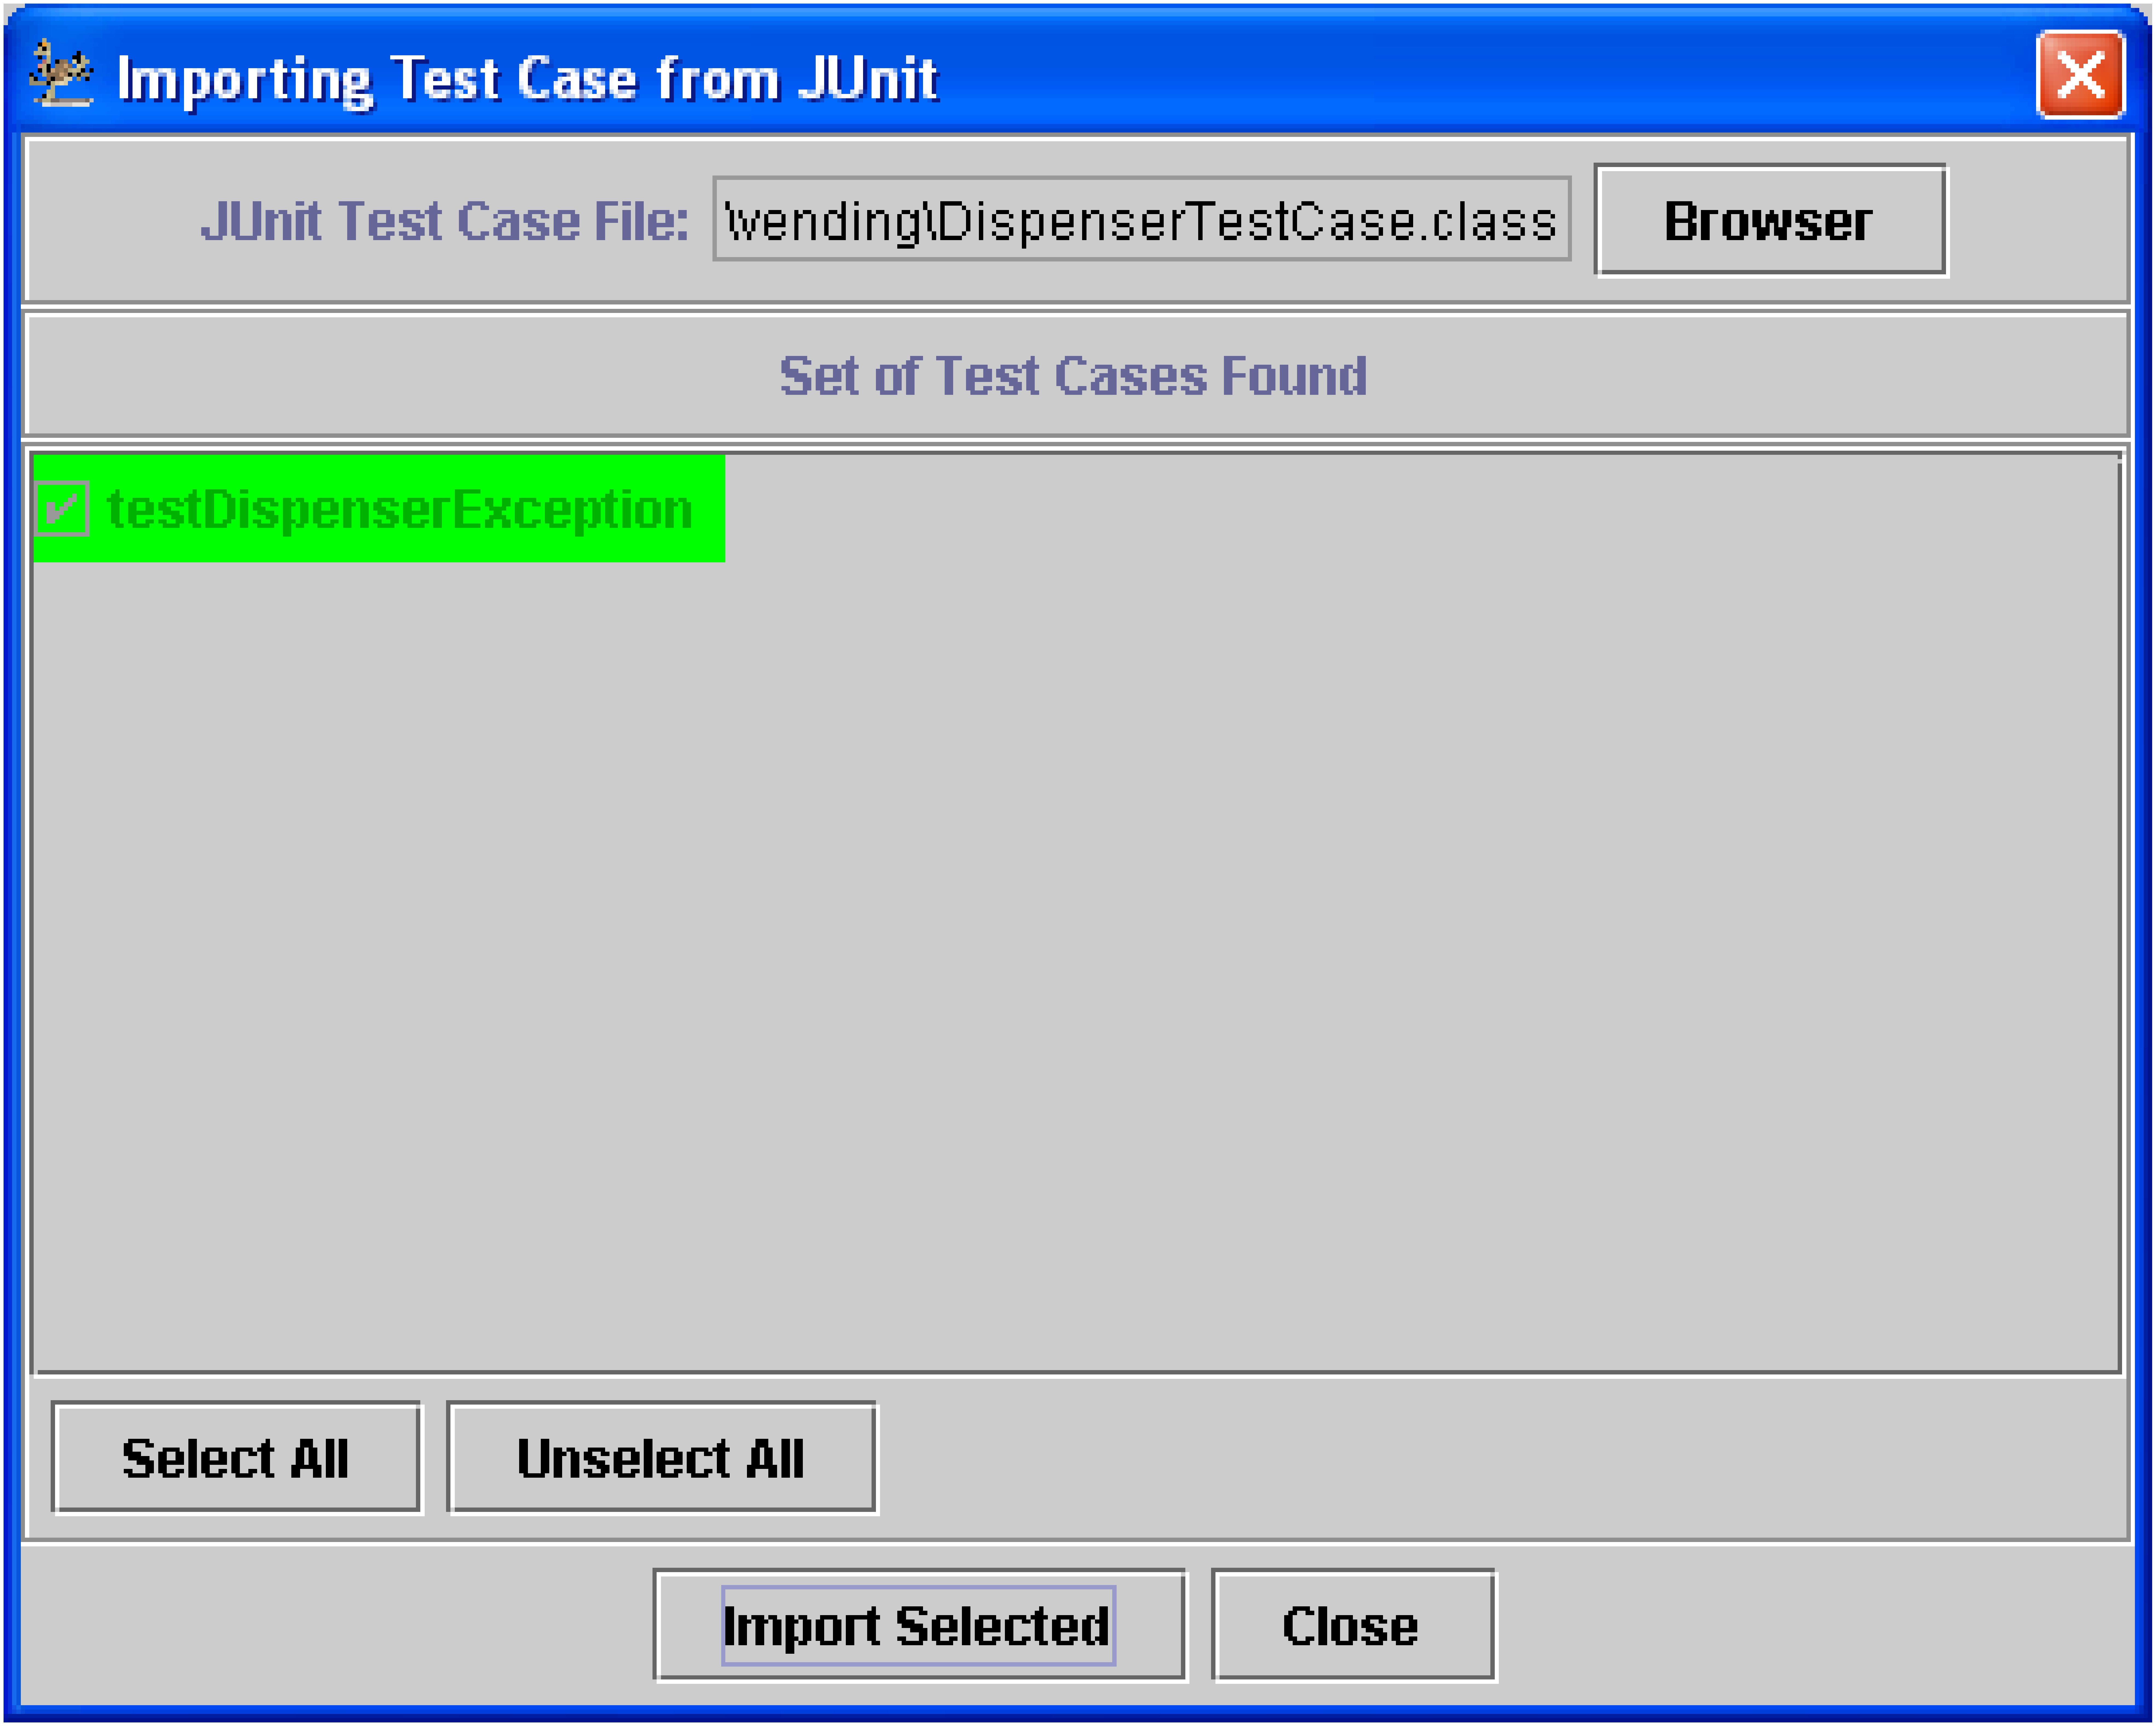
\includegraphics[width=0.45\textwidth]{fig/importing-junit-3.eps}}\quad
\caption{Sequence of Steps to Import a JUnit Test
Cases.}\label{fig:importing-junit}
\end{center}
\end{figure}


In our example (Figure~\ref{fig:junit4}), there is only one test
case to be imported. Observe that the name of such a test case
\pk{testDispenserException} is highlighted in green. This is
because JUnit framework provides several assertions statements,
like the one at line 22 of Figure~\ref{fig:junit}, that allows to
verify if the test case's output is according to its specification
or not. We use a green background color to represent test cases
that behave accordantly to their specifications and a red
background color to represent the ones that do not.

As soon as \toolname detects a new test case execution trace is
appended in the end of the trace file, the \pk{Update} button
becomes red indicating that the coverage needs to be updated.
Updated the coverage information,
Figure~\ref{fig:summary-method-tc6} shows the summary report by
methods and the corresponding coverage \wrt the \pk{All-Pri-Nodes}
criterion. The summary report by criterion can be seen in
Figure~\ref{fig:summary-criterion-tc6}

\begin{figure}[!ht]
\begin{center}
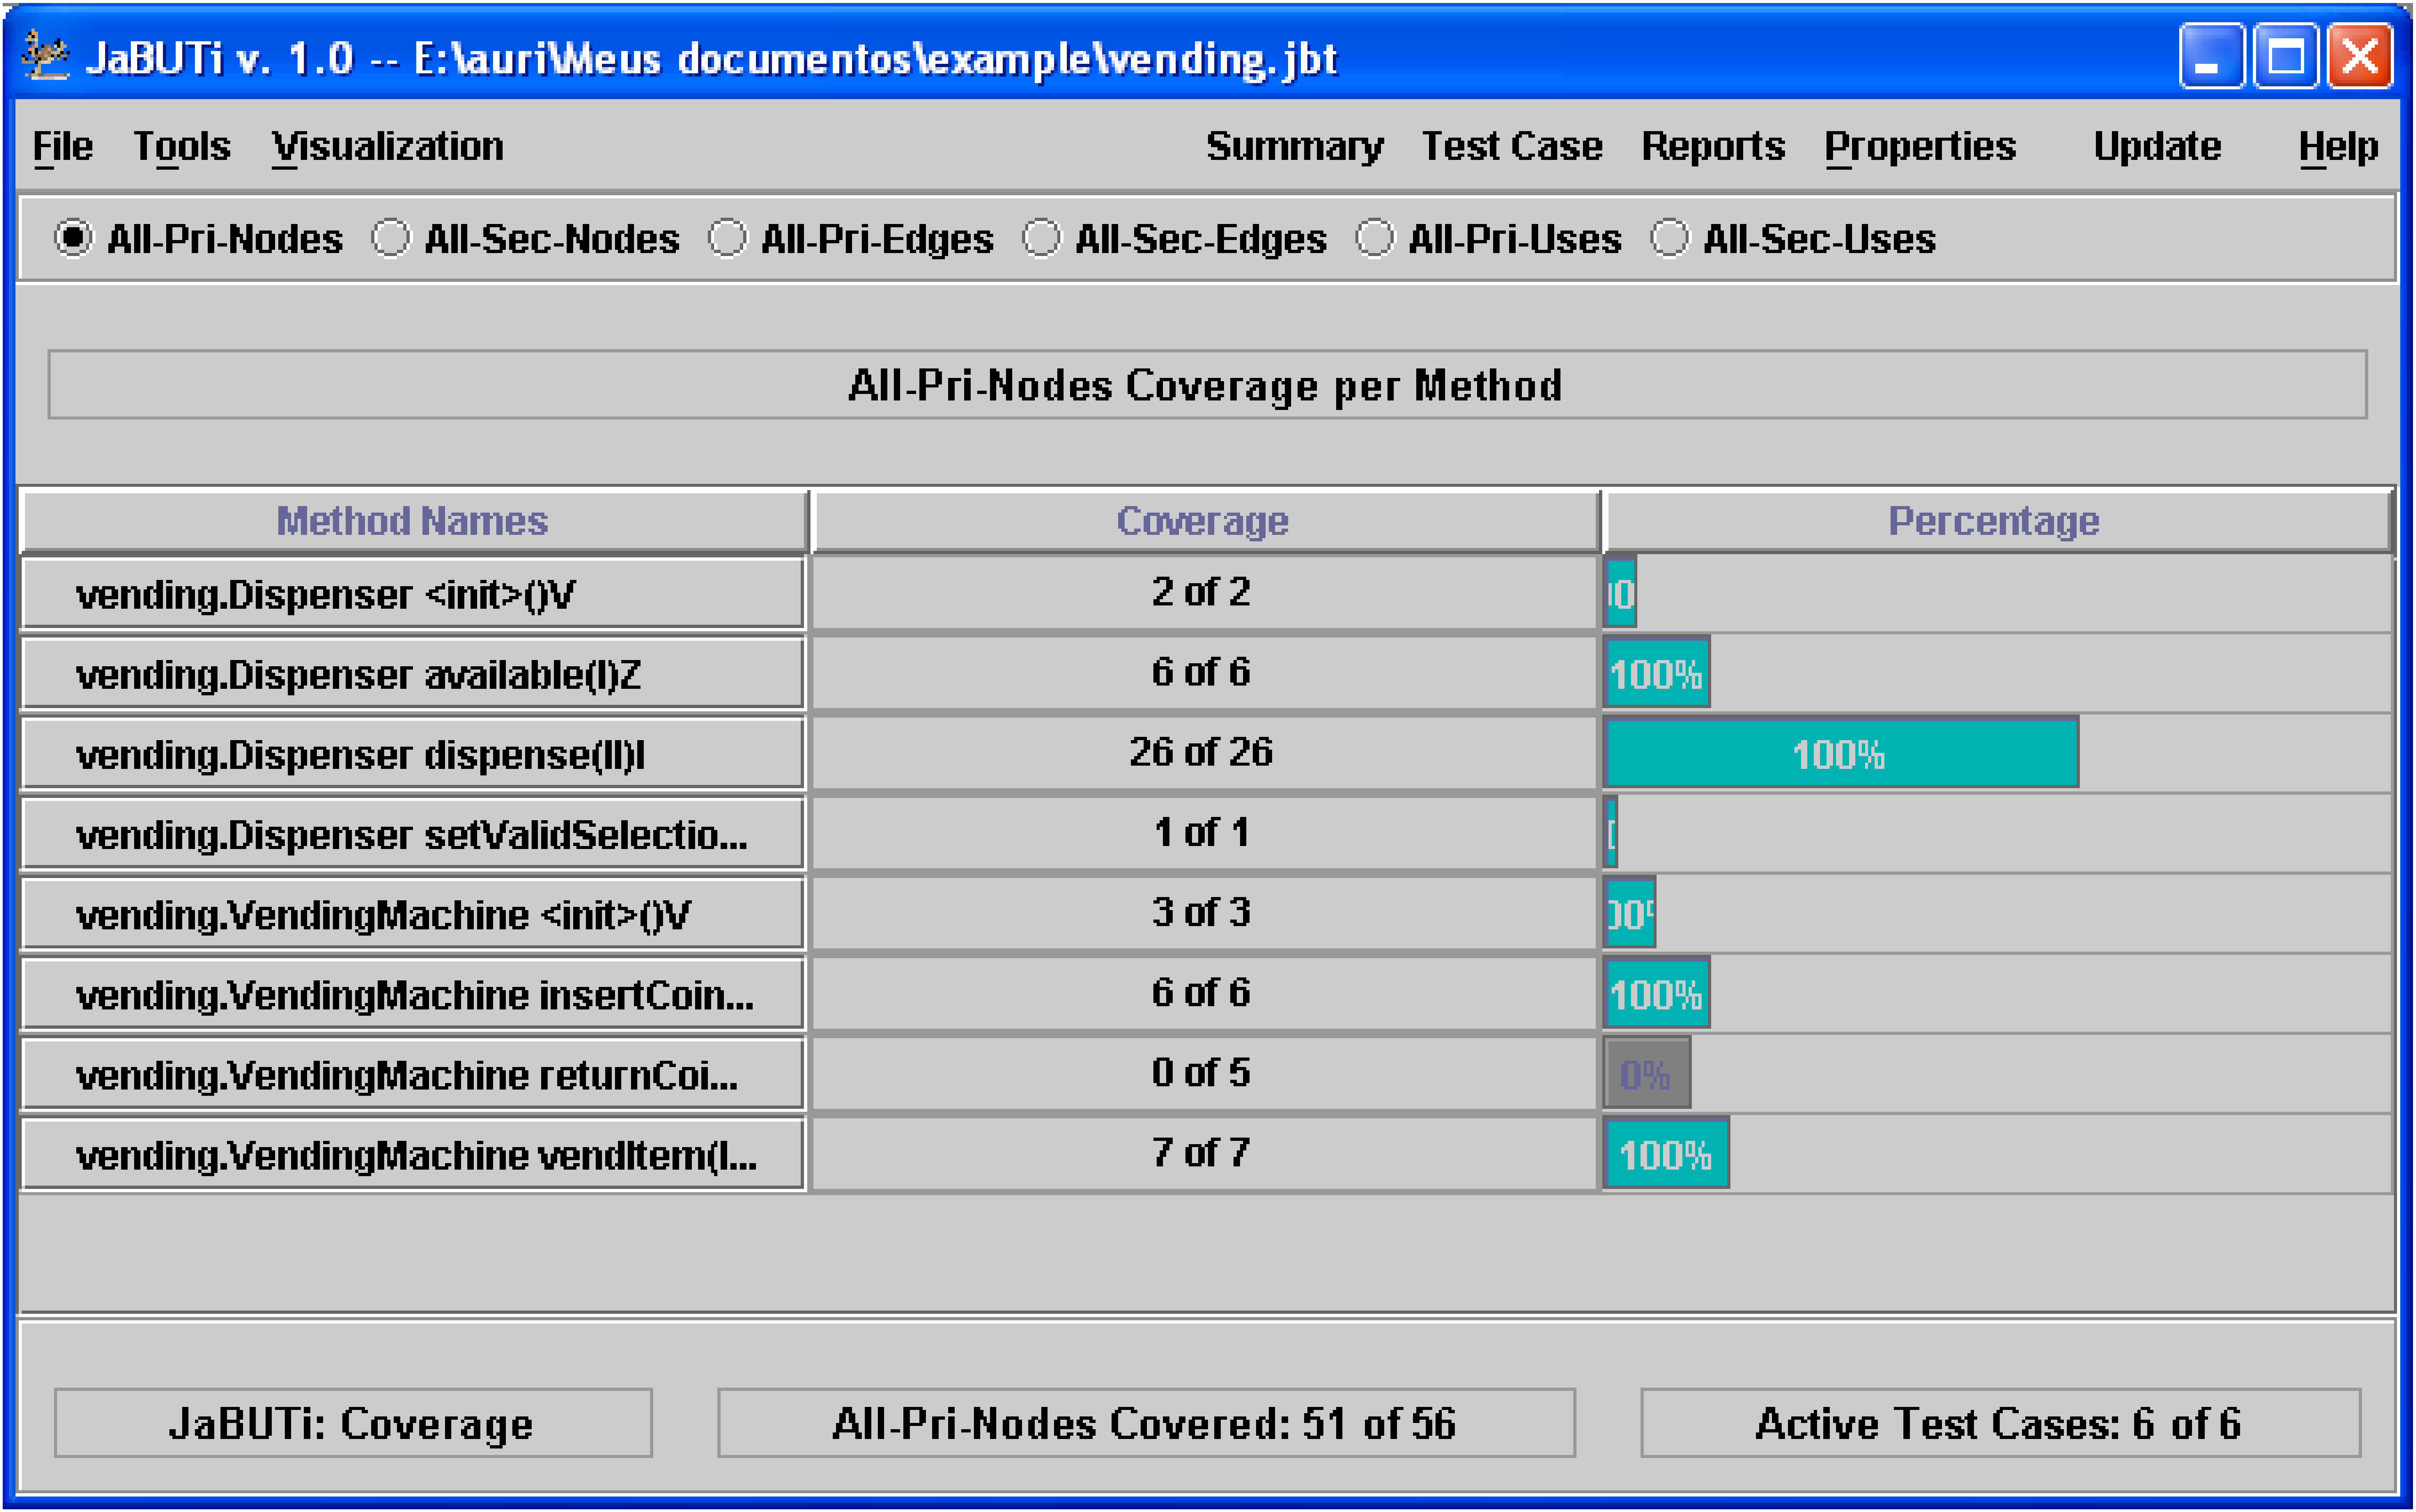
\includegraphics[width=0.70\textwidth]{fig/report-by-method-pri-nodes-tc6.eps}
\caption{\label{fig:summary-method-tc6} Updated coverage after six
test cases \wrt the \pk{All-Pri-Nodes} criterion.}
\end{center}
\end{figure}


\begin{figure}[!ht]
\begin{center}
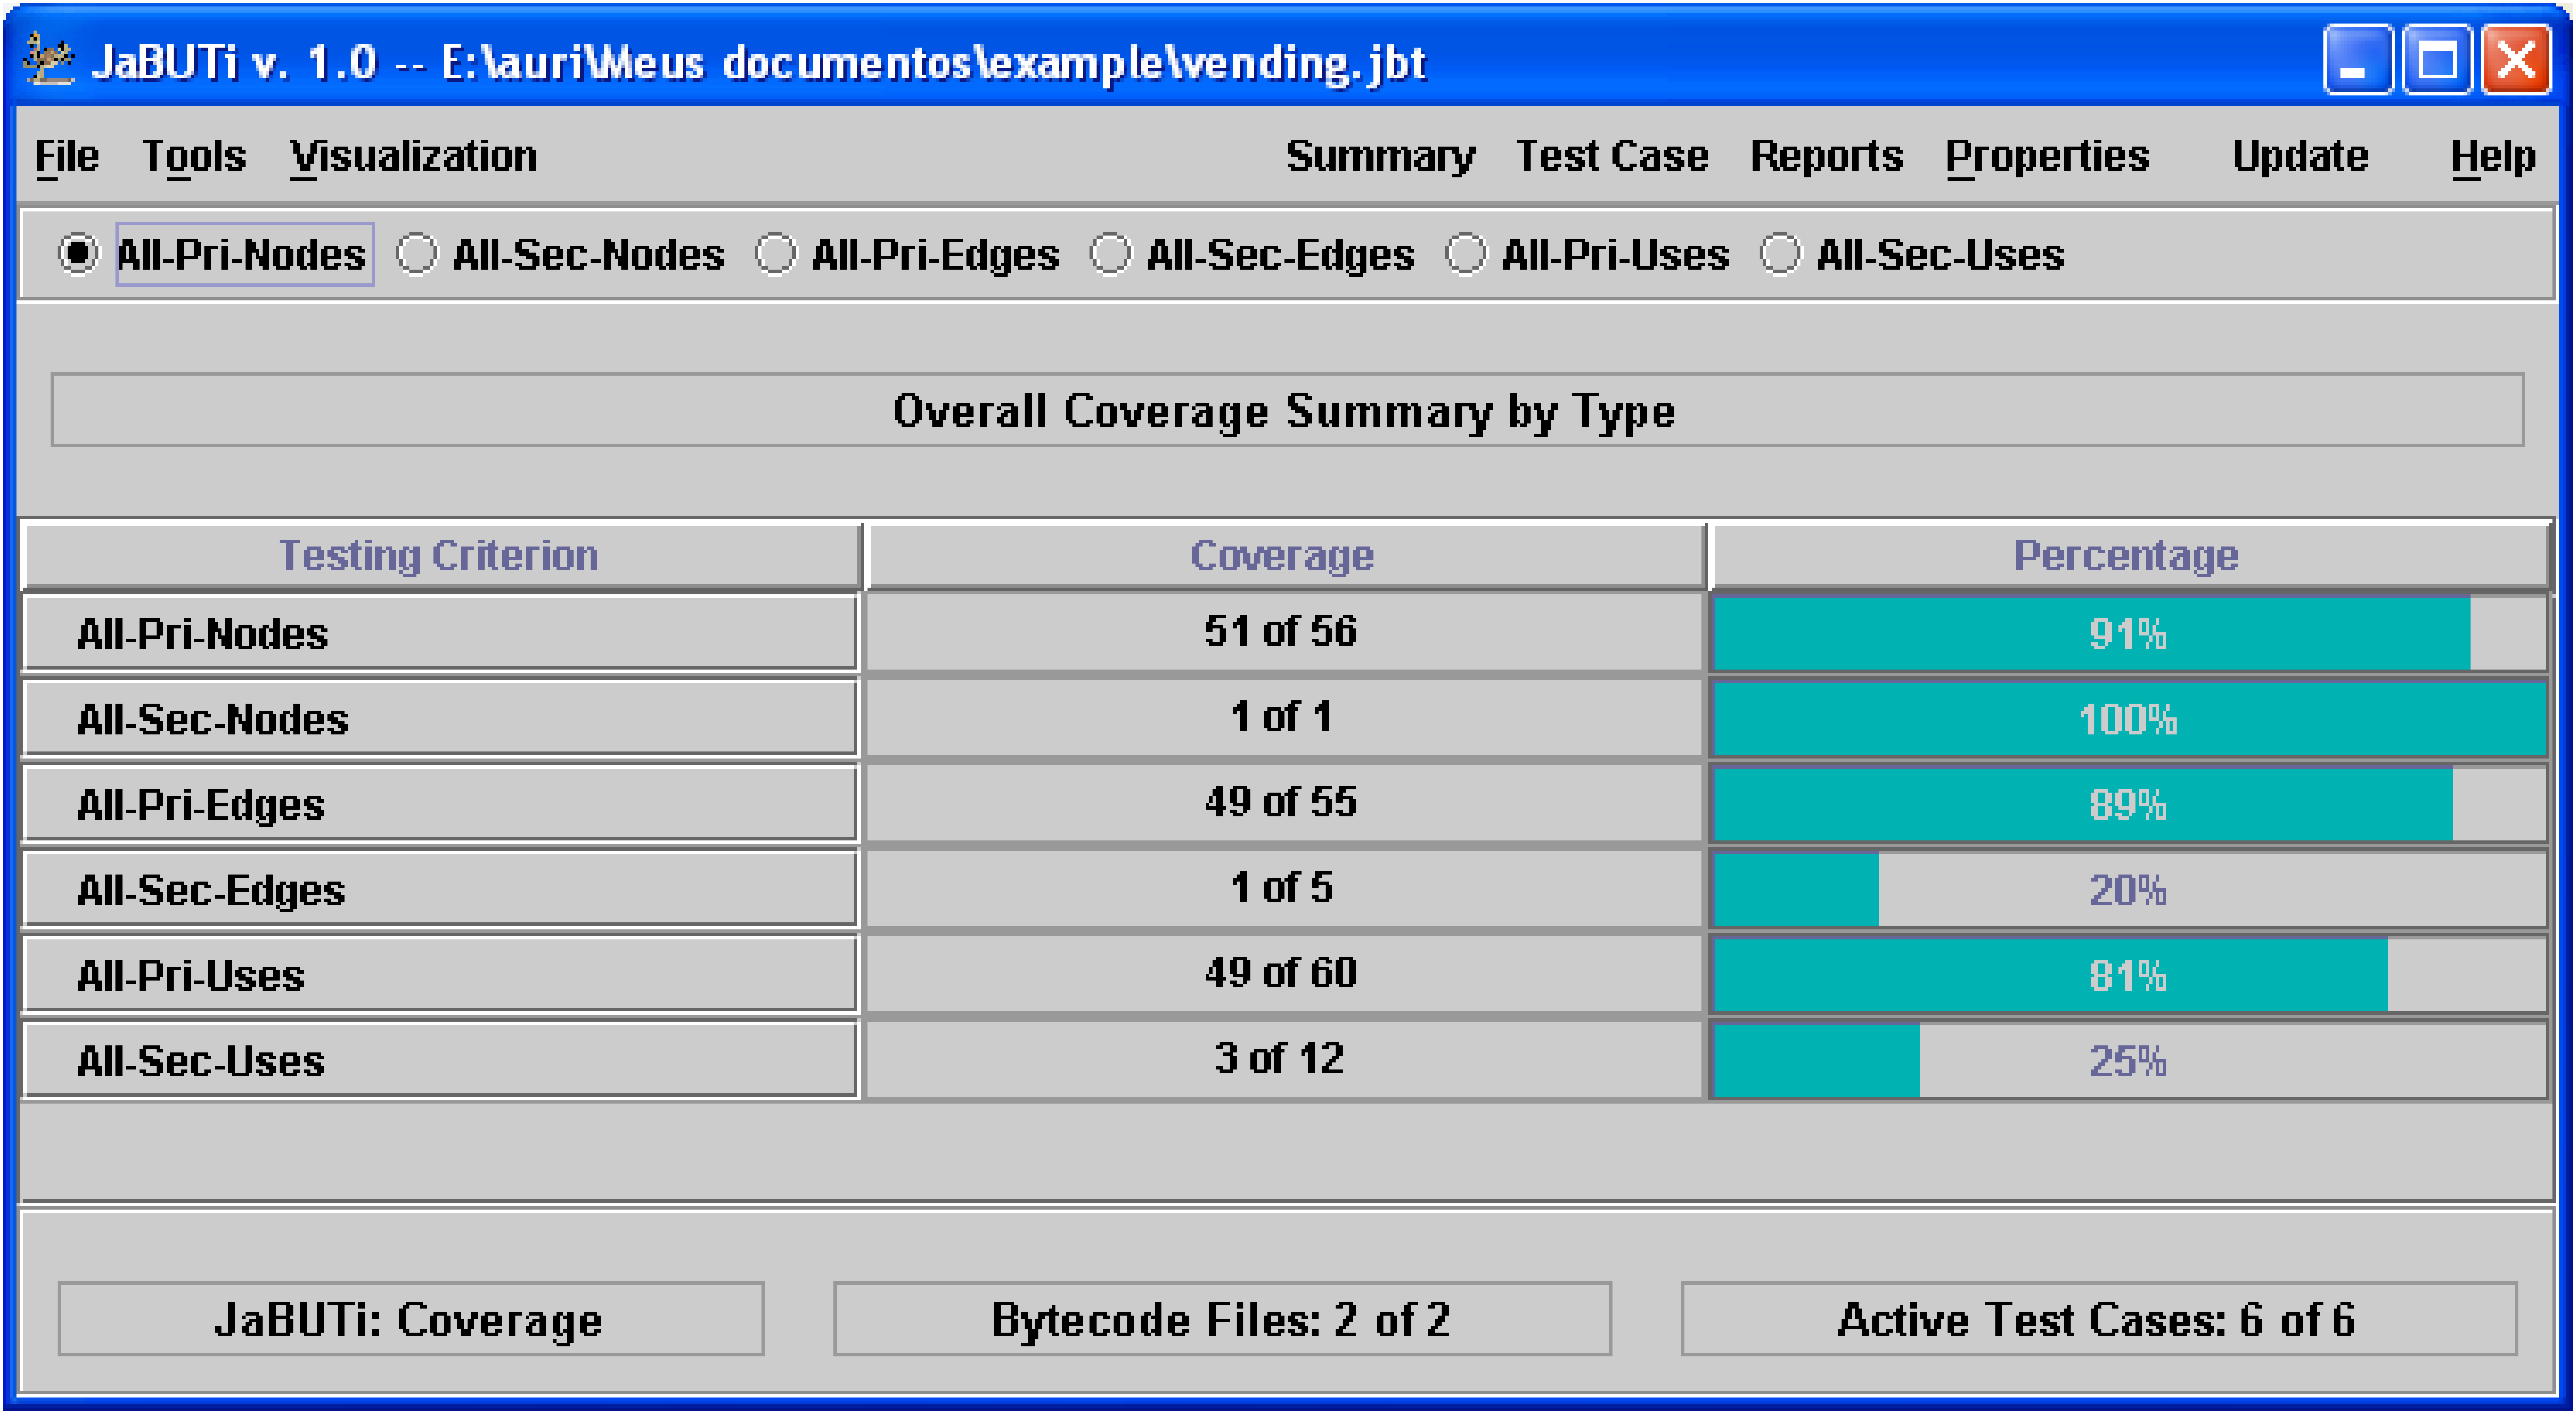
\includegraphics[width=0.70\textwidth]{fig/report-by-criterion-tc6.eps}
\caption{\label{fig:summary-criterion-tc6} Updated coverage after
six test cases \wrt all criteria.}
\end{center}
\end{figure}


After the execution of these six test cases, all methods of the
\pk{Dispenser} component are 100\% covered \wrt the
\pk{All-Pri-Nodes} criterion, but this test set is adequate to the
\pk{VendingMachine} class. More specifically, the
\pk{VendingMachine.returnCoin} method is not covered yet. So,
after six test cases, the coverage of the entire project \wrt
\pk{All-Pri-Nodes} and \pk{All-Sec-Nodes} are 91\% and 100\%,
respectively. The coverage for the \pk{All-Pri-Edges} and the
\pk{All-Sec-Edges} are 89\% and 20\%, respectively, and the
coverage for the \pk{All-Pri-Uses} and \pk{All-Sec-Uses} are 81\%
and 25\%, respectively.

Independently of the number of test cases available, if desired,
the tester can enable/disable any combination of test cases by
accessing the \pk{Test Case $\rightarrow$ Report By Test Case}
menu option and choosing which test case should be
enabled/disabled. Once a different subset of test cases are
enabled/disabled all the coverage information should be updated by
clicking on the \pk{Update} button. Figure~\ref{fig:test-case1}
shows the complete test set with all test cases enabled.
Figure~\ref{fig:test-case2} shows the updated coverage considering
only the test cases number 2 and 5.

\begin{figure}[!ht]
\begin{center}
\subfigure[]{\label{fig:test-case1}\includegraphics[width=0.45\textwidth]{fig/summary-by-test-case1.eps}}
\subfigure[]{\label{fig:test-case2}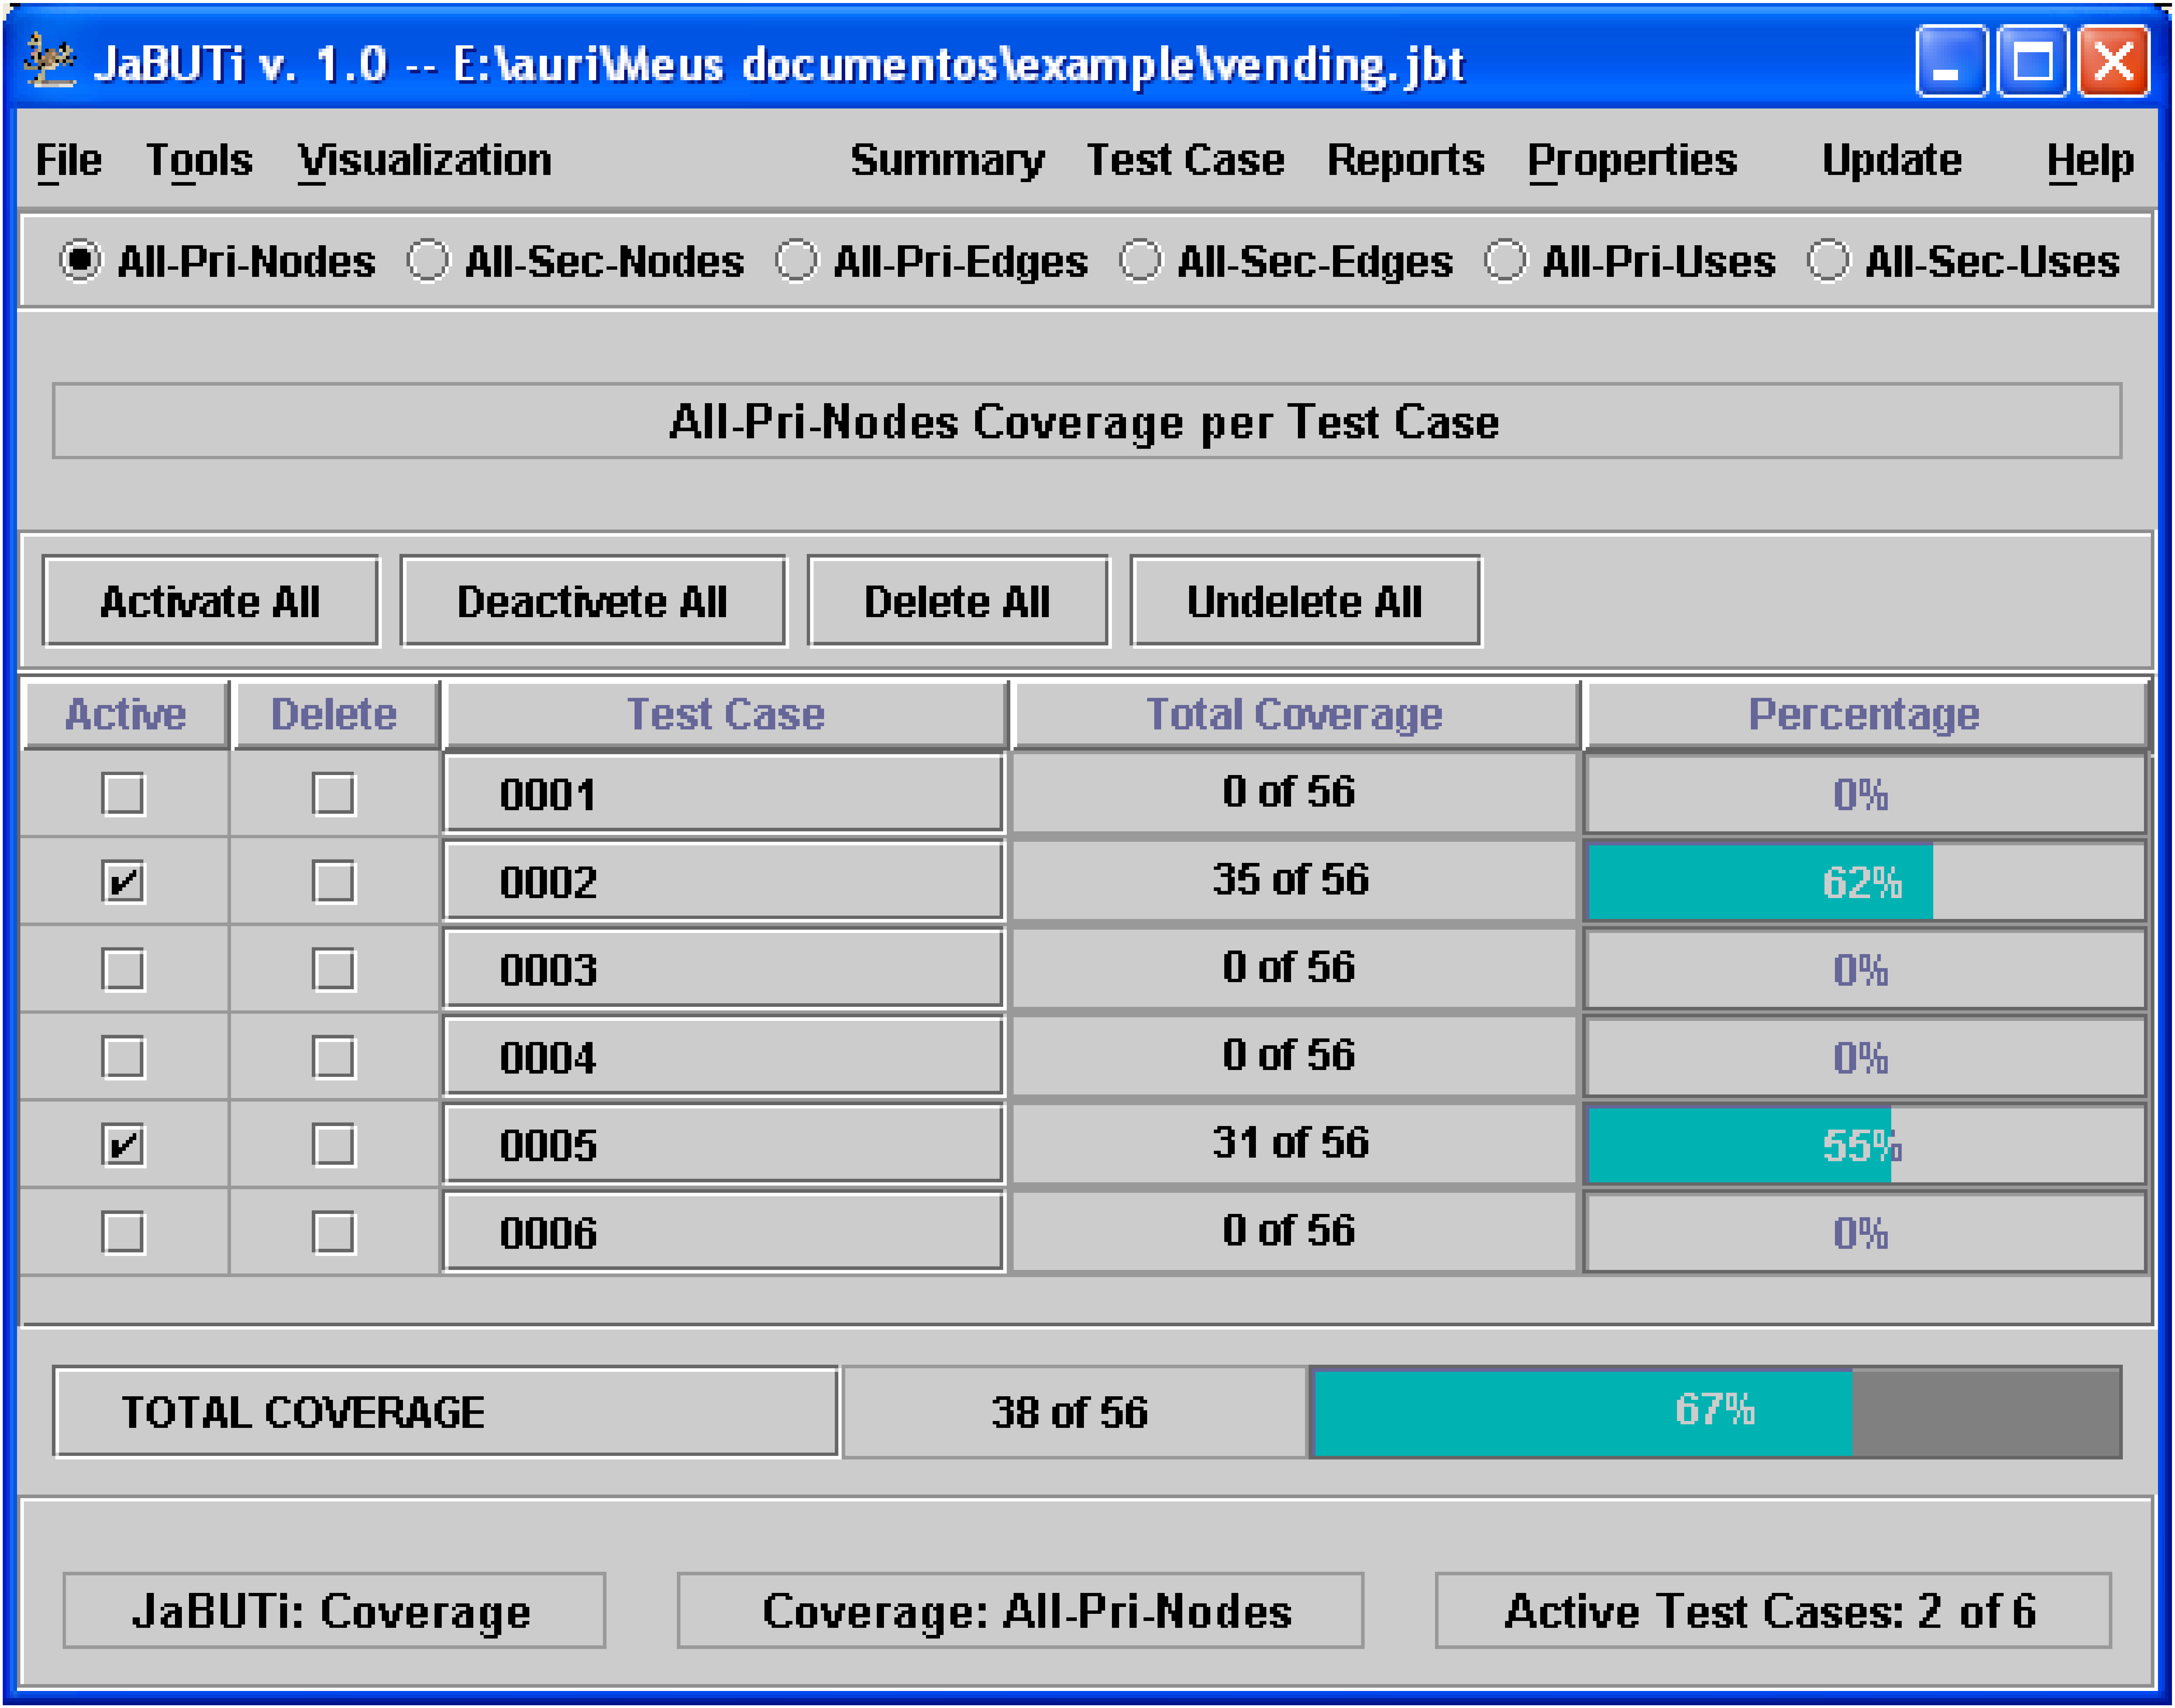
\includegraphics[width=0.45\textwidth]{fig/summary-by-test-case2.eps}}
\caption{Summary by test case: (a) all enabled, and (b) 2 and 5
enabled.}\label{fig:test-case}
\end{center}
\end{figure}


Using the resource of activate/deactivate test cases, the tester
can evaluate how the coverage changes, considering different
combinations of test case. Moreover, besides activate/deactivate
test cases, the tester can also mark a test case to be deleted.
Once a test case is marked to be deleted it is only logically
deleted. Such a test case is physically deleted when the project
is saved and closed. While the project is not closed, a test case
marked as deleted can be undeleted.

\afterpage{\clearpage}
\newpage

\subsection{How to mark a testing requirement as infeasible}

When applying structural testing criteria, one problem is to
identify infeasible testing requirements since, in general, it is
an undecidable problem. Vergilio~\cite{Vergilio97CRCA} developed
some heuristics to automatically determine infeasible testing
requirements but such heuristics are not yet implemented in
\toolname. Therefore, it is a responsibility of the tester to
identify such infeasible testing requirements.

By accessing the \pk{Visualization $\rightarrow$ Required
Elements} menu option, \toolname allows the tester to visualize
and mark testing requirements as infeasible, as well as
activate/deactivate testing requirements. Once a testing
requirement is marked as infeasible or deactivated, the
\pk{Update} button becomes red indicating that the coverage
information should be updated to reflect such a change. For
example, Figure~\ref{fig:requirements} shows part of the testing
requirements for the method \pk{Vending.returnCoin()} method,
considering the \pk{All-Pri-Nodes} criterion.

\begin{figure}[!ht]
\begin{center}
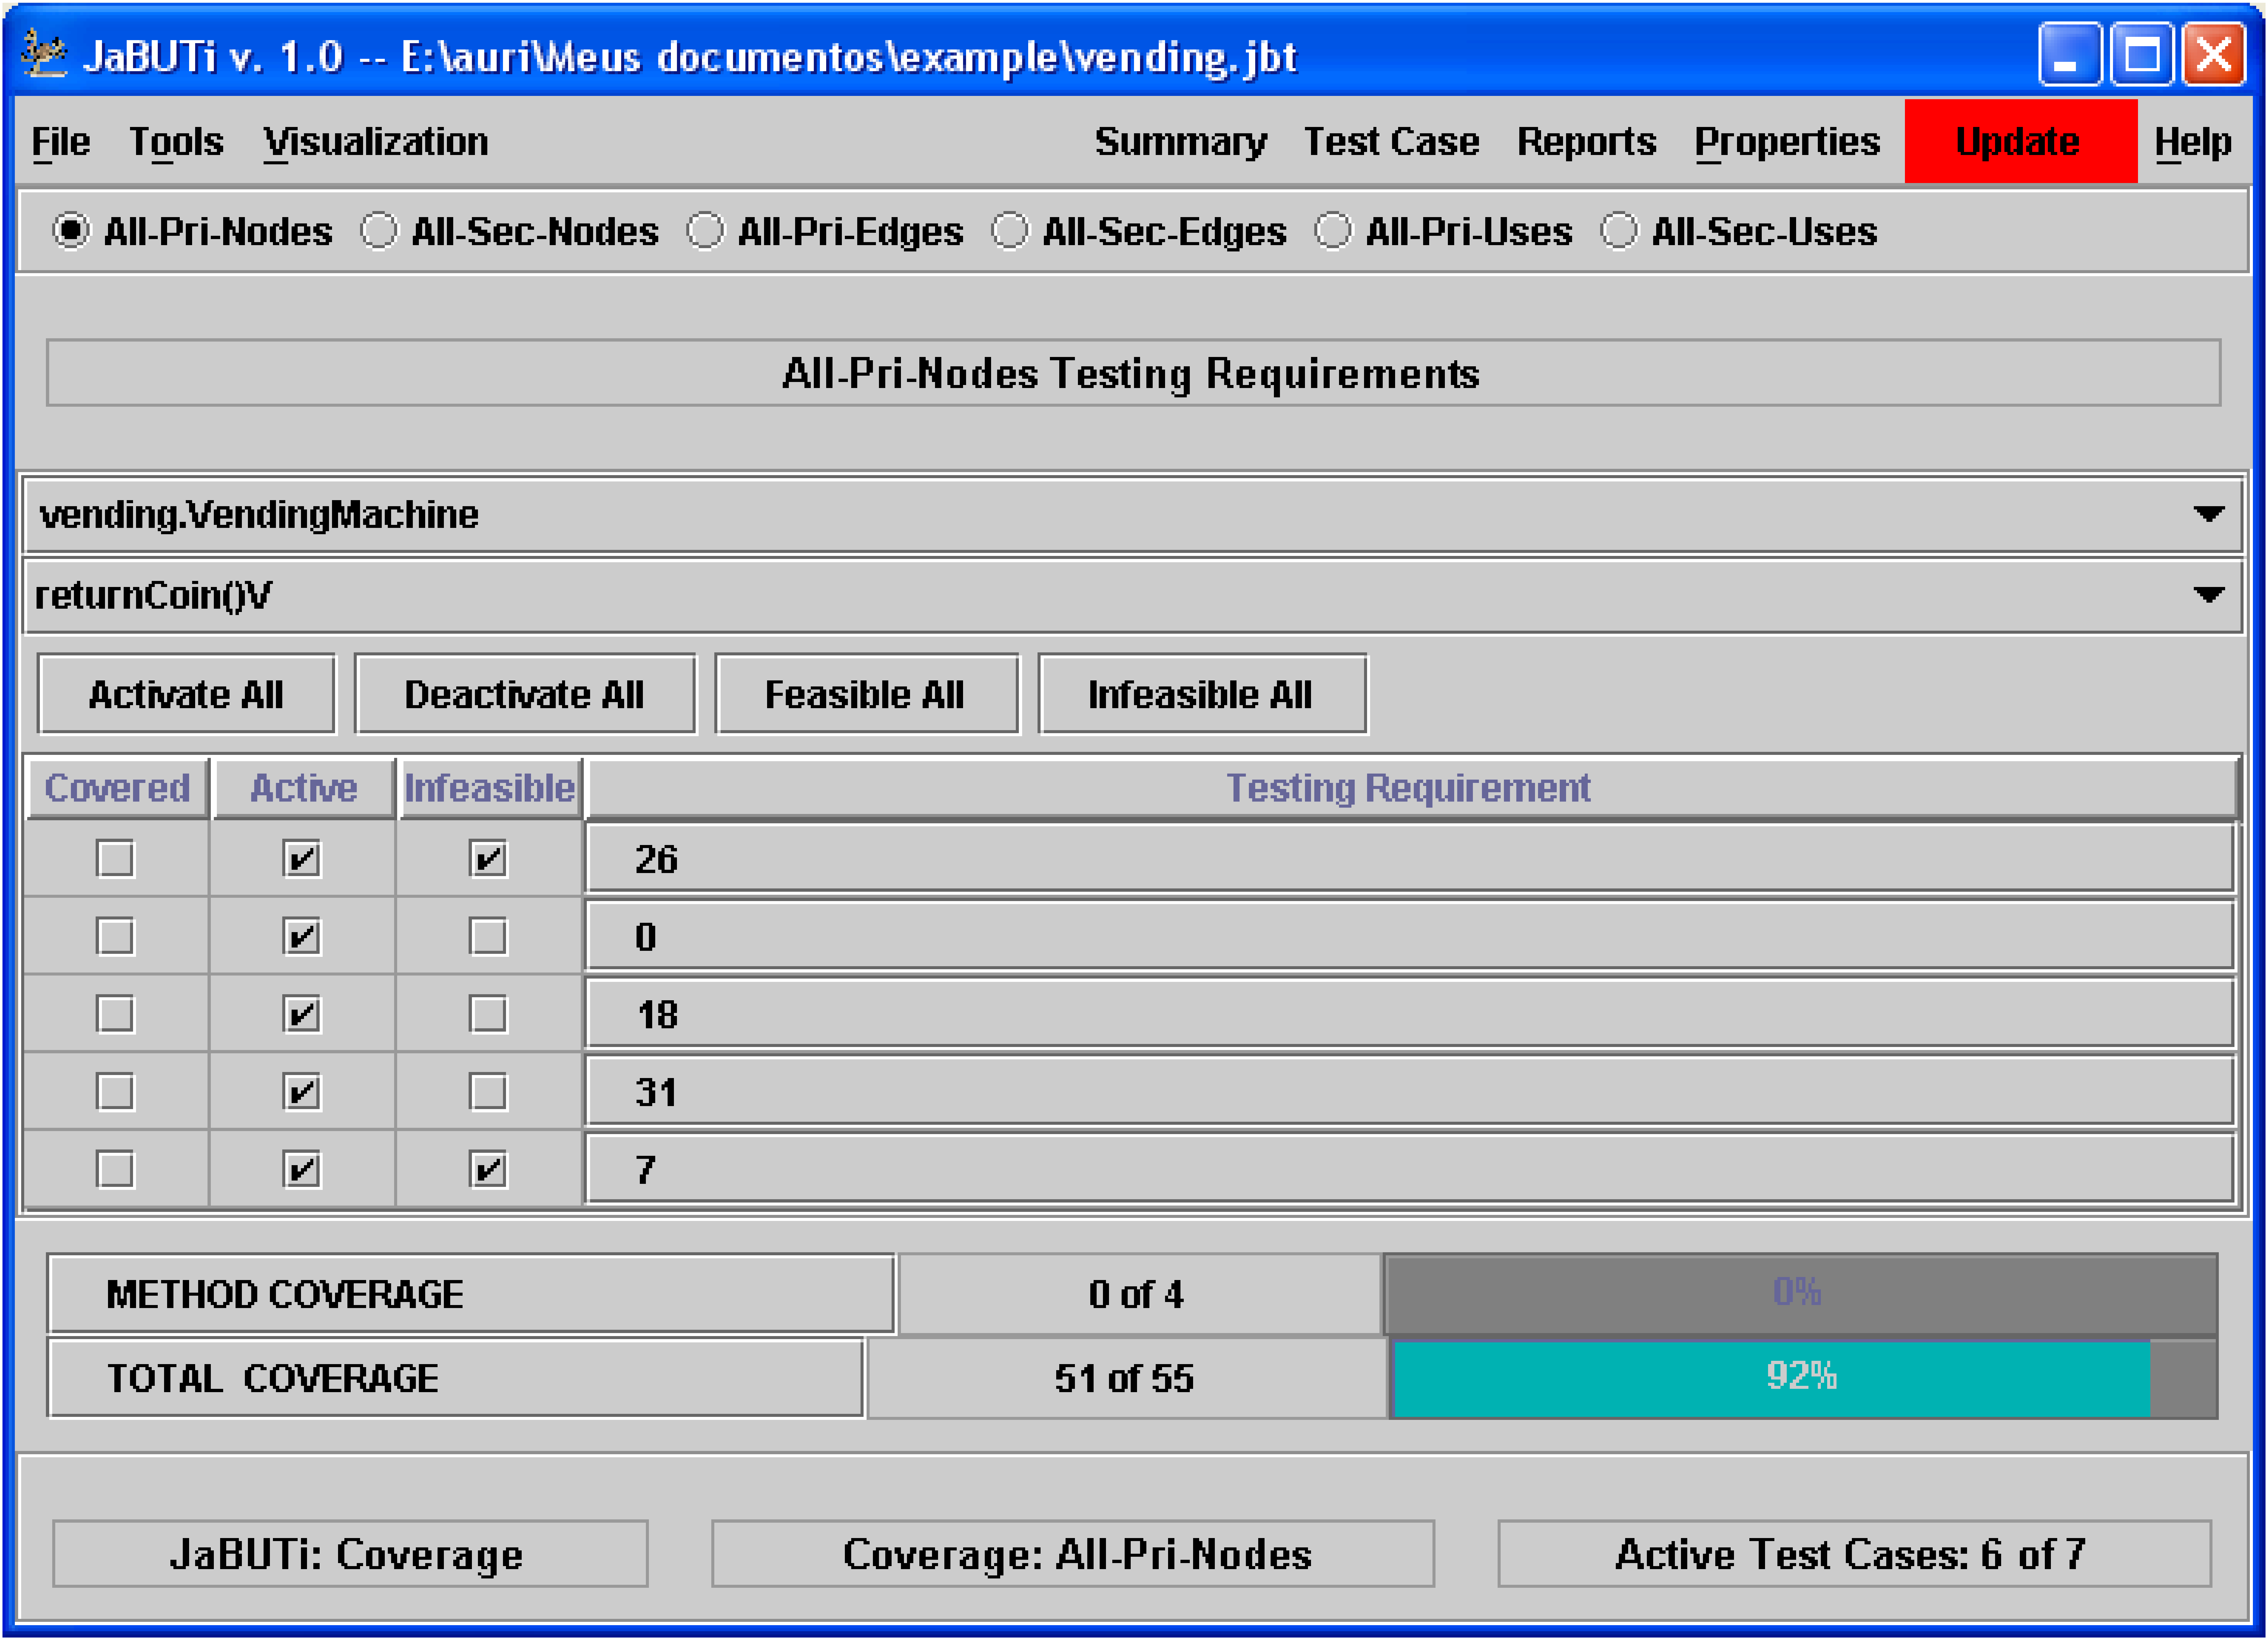
\includegraphics[width=0.70\textwidth]{fig/required-elements.eps}
\caption{\label{fig:requirements} \pk{Dispenser.dispense()}
required elements for the \pk{All-Pri-Nodes} criterion.}
\end{center}
\end{figure}


Considering Figure~\ref{fig:requirements}, two uncovered
requirements were marked as infeasible, primary nodes 7 and 26.
Since the tester can mark erroneously a testing requirement as
infeasible, in case such a testing requirement is covered in the
future by an additional test case, the tool indicates such a
inconsistency, highlighting the infeasible check box of a covered
testing requirement in red, as illustrated in
Figure~\ref{fig:covered-infeasible}. In this case, primary node 26
is covered by the new test case added to exercise the
\pk{Vending.returnCoin()} method, so node 26 is feasible.

During the importation of a given test case, the tester has to
check whether the obtained output is correct \wrt the
specification. As can be observed in Table~\ref{tab:adequate},
only test case number 1 does not behave according to the
specification. Once any discrepancy is detected, the fault should
be localized and corrected. One alternative for fault localization
is slicing. In the next section we describe how to use the slicing
tool implemented in \toolname to help the fault localization and
smart debugging.

\begin{figure}[!ht]
\begin{center}
\includegraphics[width=0.70\textwidth]{fig/required-elements-covered-infeasible.eps}
\caption{\label{fig:covered-infeasible} \pk{Dispenser.dispense()}
infeasible requirements erroneously identified.}
\end{center}
\end{figure}


\afterpage{\clearpage}
\newpage
